\documentclass[logos,chaptertoc]{bordeaux-thesis}

%########################################################################
% Extensions
%########################################################################

%Text encoding and fonts
\usepackage[utf8]{inputenc}
\usepackage[T1]{fontenc}
%\usepackage{graphicx}


%########################################################################
% Title page
%########################################################################

%Thesis author
\author{Christophe \textsc{Cossou}}

%Title for main language (french)
\title{Migration et accrétion d'embryons planétaires dans un disque radiatif}
%Titles for other languages
\title[english]{My English thesis title}


%Keywords for main language (french)
\keywords{Blabla, blabla, blabla, blabla, blabla, blabla, blabla}
%Keywords for other languages languages
\keywords[english]{Blabla, blabla, blabla, blabla, blabla, blabla, blabla}

%Order number of the thesis
\ordernumber{1234}

%Date of defense
\date{xx Xxxxxxxxx xxxx}
\submityear{2013}

%You define the commission member list using \addcommissionmember (mandatory) with an optional role (eg: president, supervisor, etc...)
\addcommissionmember{Aaaaa}{Bbbbbbbb}{Astronome, Université Paris VI, LESIA}{Président du Jury}
\addcommissionmember{Ccccccccc}{Dddddddddd}{Directeur de recherche, Université Bordeaux 1, LAB}{Directeur de thèse}
\addcommissionmember{Eee}{Fffff}{Maître de conférence, Université Bordeaux 1, LAB}{Examinateur}
\addcommissionmember{Ggggggggg}{Hhhhhhh}{Professeur, Aix-Marseille, Université OAMP}{Examinateur}
\addcommissionmember{Iiii}{Jjjjjjjjjjjj}{Professeur, Aix-Marseille, Université OAMP}{Examinateur}
\addcommissionmember{Kkkkkkkkkkkk}{Llllll}{Professeur, Aix-Marseille, Université OAMP}{Examinateur}

%If some referees are not part of the commission, you can add them in a separate list with \addreferee (optional)
\addreferee{Mmmmmmmm}{Nnnnnnnn}{Professeur, Aix-Marseille, Université OAMP}
\addreferee{Oooooooooo}{Pppppppp}{Maître de conférence, Université Bordeaux 1, LAB}
%\addreferee{toto}{Pppppppp}{Maître de conférence, Université Bordeaux 1, LAB}

\newcommand{\dummytext}{
Lorem ipsum dolor sit amet, consectetuer adipiscing elit. Phasellus blandit massa non tellus. Pellentesque blandit. Etiam sapien. Quisque sed massa ac tortor accumsan bibendum. Donec et orci quis mi sollicitudin consectetuer. Donec malesuada. Pellentesque bibendum pellentesque elit. Morbi et diam ac wisi auctor fringilla. Cras nec arcu sed velit dapibus blandit. Maecenas mollis aliquet quam. In eget sem nec orci fringilla sagittis. Suspendisse cursus placerat massa. Pellentesque non metus. Morbi congue tellus eget tellus. Suspendisse justo. Suspendisse potenti. Praesent interdum lorem in velit. Nullam sit amet nisl eget wisi consectetuer consequat. Mauris vel felis. Nulla sed neque.

Nulla facilisi. Maecenas accumsan gravida wisi. Maecenas sodales gravida neque. Mauris in est a ante molestie gravida. In id neque. Ut augue. Duis fringilla ullamcorper risus. Nullam at lorem. Quisque consequat turpis ac libero. Ut auctor ante commodo magna. Donec in magna. Integer sodales. Donec ac nibh eu felis suscipit elementum.

Fusce convallis dolor sit amet dolor. Nulla sit amet pede. Maecenas et ante vitae risus tempus facilisis. Nullam ut tellus et lacus sollicitudin condimentum. Maecenas vitae lorem. Quisque nec leo varius est euismod posuere. Integer ac diam in enim pellentesque pulvinar. Etiam sodales tristique eros. Curabitur non magna. Suspendisse blandit metus vitae purus. Phasellus nec sem vitae arcu consequat auctor. Donec nec dui. Donec sit amet lorem vel erat tristique laoreet. Duis ac felis tincidunt arcu consequat faucibus. Vestibulum ultrices porttitor purus. In semper consequat dolor. Nunc porta. Vestibulum nisl ipsum, rhoncus quis, adipiscing sed, sollicitudin ut, quam.
}


%########################################################################
% Document start
%########################################################################

\begin{document}

%Print title NOW
\maketitle%

%Disable page numbering
\pagestyle{empty}

%########################################################################
% Multilingual abstracts
%########################################################################

%French abstract:
\begin{abstract}
\dummytext
\end{abstract}

%Horizontal rule
\noindent\hspace*{0.35\textwidth}\hrulefill\hspace*{0.35\textwidth}\\[-\bigskipamount]

%English abstract:
\begin{abstract}[english]
\dummytext
\end{abstract}

%########################################################################
% Acknowledgments
%########################################################################

\pagebreak\strut\newpage

\chapter*{Remerciements}
%Put the text vertically centered
\vfill
\dummytext

%TODO citation kaamelott?
% épisode le repos du guerrier II, de la saison 3 (3x37), perceval parle de l'espace

\newpage

%########################################################################
% Contents
%########################################################################

\strut\newpage

\tableofcontents

\newpage

%########################################################################
% Introduction
%########################################################################

%Enable page numbering
\pagestyle{fancy}

\chapter*{Introduction}
\addstarredchapter{Introduction}% To be used instead of addcontentsline in order to have the good minitoc. If not, the starred chapter create a shift in the minitocs.
%%\addcontentsline{toc}{chapter}{Introduction}

%TODO parler de formation planétaire (en citant des papiers, sans rentrer dans les détails. notamment pollack, alibert)

%TODO une des grandes questions c'est  : comment on forme des noyaux de jupiter et Kepler 11?





\chapter{Physique des disques}
\section{Formation stellaire}
Les étoiles se forment à partir de l'effondrement gravitationnel d'un nuage de gaz. Quand ce dernier est suffisamment massif (masse au delà d'une masse critique dite masse de Jeans, de l'ordre de quelques masses solaires, même si ça dépend de la configuration, du volume etc\dots), son autogravité initie un effondrement du nuage sur lui-même, qui peu à peu se fragmente en système découplés. 

Au centre de chaque fragment se forme un cœur pré-stellaire à mesure que la température et la pression augmentent, jusqu'à atteindre les conditions nécessaires à l'allumage de la fusion de l'hydrogène. On obtient alors une protoétoile appelée \og classe 0\fg. 

Durant l'effondrement du nuage, la conservation du moment cinétique empêche la contraction du nuage, en particulier dans le plan perpendiculaire à l'axe de rotation du nuage. Ceci ajouté à la pression de radiation, apparue depuis la formation de la protoétoile conduit à la formation d'un tore autour de l'étoile centrale en quelques dizaines de milliers d'années. Ce stade est appelé \og classe I\fg.

Le tore de gaz est chaud et par conséquence enflé, principalement à cause de l'énergie gravitationnelle résiduelle, mais aussi par le chauffage de la protoétoile centrale.
En quelques centaines de milliers d'années, ce tore devient un disque, à mesure que le rayonnement de corps noir évacue l'énergie par la surface. À mesure que le tore refroidit, et compte tenu de la conservation du moment cinétique qui empêche une contraction rapide dans le plan perpendiculaire à l'axe de rotation, il s'aplatit jusqu'à former un disque \citep{williams2011protoplanetary}. 

Un million d'années environ après la formation de la protoétoile, le disque mince est formé et la protoétoile est devenue une étoile T Tauri (objet de classe II). Après quelques millions d'années (typiquement, 10 millions d'années), le disque se dissipe et on est dans le cas d'étoiles T-Tauri évoluées ou objets de classe III. 

Ces dénominations en classe peuvent sembler étranges mais elles proviennent en premier lieu de l'étude des spectres d'étoiles jeunes qui présentent différentes caractéristiques en fonction du stade d'évolution de l'étoile. \reffig{fig:star_formation} résume la formation stellaire, les différentes phases et en particulier les caractéristiques du spectre d'émission de ces objets.
 
\begin{figure}[htbp]
\centering
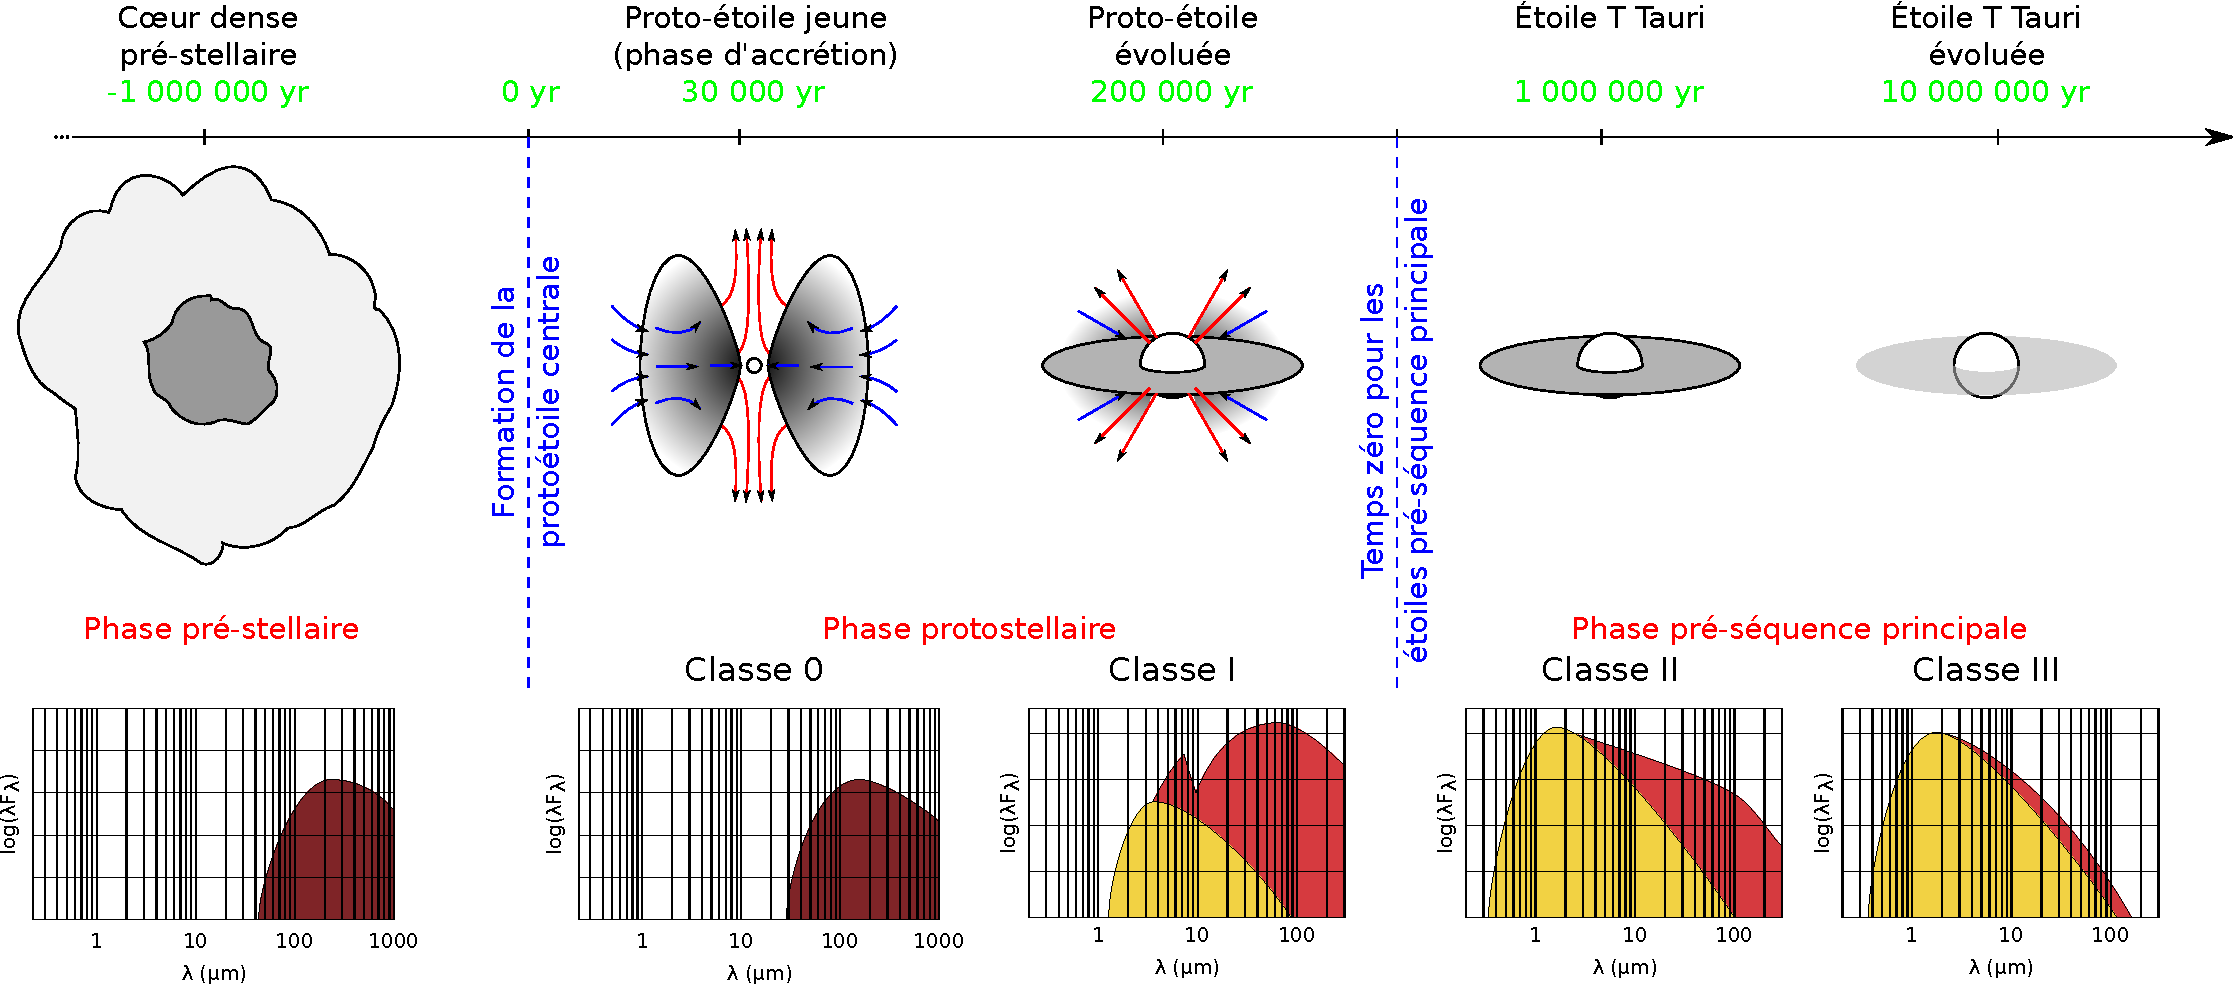
\includegraphics[width=\linewidth]{figure/star_formation.pdf}
\caption[Stades de formation d'une étoile]{Classification empirique des différents stades de formation des étoiles de faible
masse, du cœur dense pré-stellaire à la classe III. Schéma basé sur \citep{andre2002initial}. }\label{fig:star_formation}
\end{figure}


\section{Les disques protoplanétaires}
\subsection{Formation et évolution}
Durant les différentes phases de formation de l'étoile, alors même que le disque de gaz et de poussière se dissipe a lieu la formation des planètes. 

À mesure que le nuage s'effondre sur lui-même, et afin de satisfaire à la conservation du moment cinétique, ce dernier voit sa rotation accélérer, même si la rotation du nuage moléculaire était infime au départ. C'est ainsi que le disque d'accrétion, résultat de l'effondrement du nuage de gaz, est en rotation. L'effondrement d'un nuage moléculaire s'effectuant sur plusieurs ordres de grandeur (en distance), l'accélération de la rotation est d'autant plus grande.

Initialement, il est hautement improbable que le moment cinétique du nuage soit parfaitement nul. C'est ainsi que même si sa rotation est imperceptible lors des premiers stades de son effondrement gravitationnel, le disque d'accrétion fini toujours en rotation. 

\subsection{Évolution hydrodynamique du disque}
\begin{figure}[htbp]
\centering
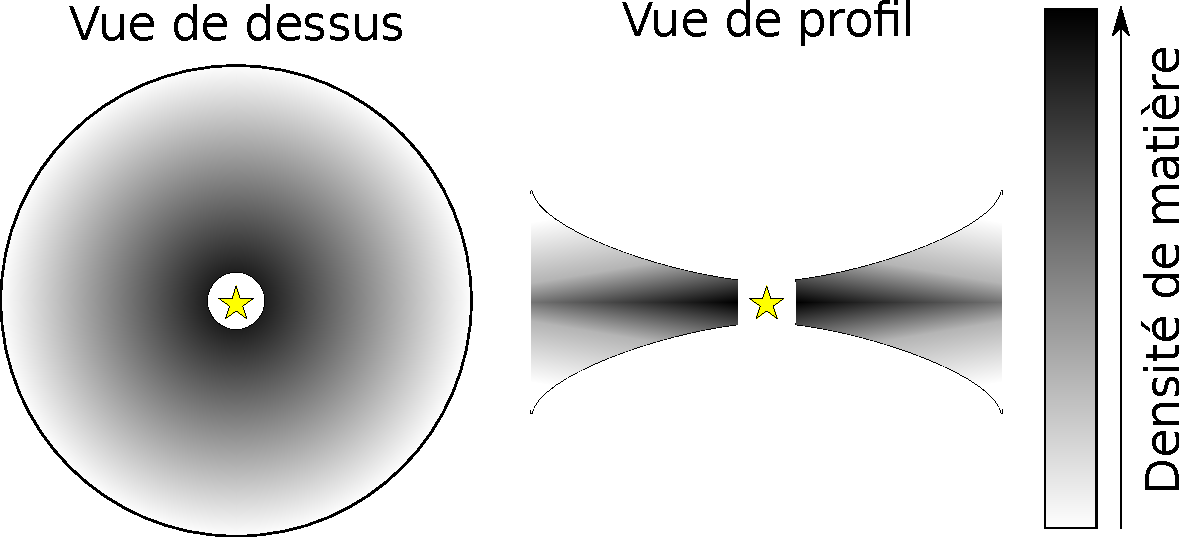
\includegraphics[width=0.6\linewidth]{figure/disk_scheme.pdf}
\caption[Vue de face et de profil d'un disque de gaz.]{Représentation de la répartition radiale et azimutale
de gaz dans un disque protoplanétaire.}\label{fig:disk_scheme}
\end{figure}

Avant de considérer l'évolution d'un disque, il est important de regarder sa masse par rapport à la masse de l'étoile centrale. En effet, si la masse du disque est de l'ordre de la masse de l'étoile, alors des instabilités se développent et on ne peut plus négliger l'autogravité du disque. 

Le \gras{paramètre de Toomre} $Q$, défini par \citep{toomre1964gravitational, goldreich1965gravitational}:
\begin{align}
Q &= \frac{\kappa c_{s}}{\pi G \Sigma}
\end{align}
est un indicateur de la stabilité du disque par rapport à l'auto-gravité. $\kappa$ est la fréquence épicyclique, $c_s$ la vitesse du son, $G$ la constante de gravitation universelle et $\Sigma$ la densité de surface. 

Dans ce paramètre, $\pi G \Sigma$ représente la masse du disque. La vitesse du son $c_{s}$ est liée à la pression thermique ; la \gras[fréquence!epicyclique@épicyclique]{fréquence épicyclique} $\kappa$ détermine quant à elle la force du cisaillement dans le disque.

\bigskip

Si $Q<1$ alors le gaz est instable gravitationnellement et il commence à s'effondrer sur lui-même et former des sur-densités à condition que le temps de refroidissement soit inférieur à 3 fois la période orbitale ($\tau_c \lesssim 3 \Omega^{-1}$) \citep{gammie2001nonlinear}.
Si $Q>1$, le disque est stable.

À partir du paramètre $Q$, on peut dériver une condition sur le rapport de masse entre étoile et disque pour que l'auto-gravité soit négligeable, ce qui donne \citep{gammie2001nonlinear} : 
\begin{align}
\frac{M_\text{d}}{M_\star} &\lesssim \frac{H}{R}
\end{align}
où $M_\text{d}$ et $M_\star$ sont respectivement la masse du disque et de l'étoile. $H$ est l'échelle de hauteur du disque et $R$ la distance par rapport à l'étoile.

Nous ne considérerons que des disques dont la masse $M_\text{d}$ est faible devant la masse de l'étoile $M_\star$. Si tel n'était pas le cas, le temps pour que le disque perde suffisamment de masse pour se retrouver dans le cas qui nous intéresse sera court devant la vie du disque et le temps de formation planétaire. Étant donné qu'on ne s'intéresse qu'aux derniers stades de la formation planétaire, à savoir quand les embryons planétaires ont une masse de l'ordre du dixième de masse terrestre au minimum, il est raisonnable de penser que le disque sera dans un stade peu dense où l'approximation $Q>1$ sera valable.

Dans un tel cas, c'est le potentiel gravitationnel de l'étoile qui domine la dynamique du gaz. En négligeant l'effet de la pression de ce dernier, on peut donc écrire la vitesse angulaire du gaz comme étant égale à la vitesse angulaire képlerienne : 
\begin{align}
\Omega &= \sqrt{\frac{GM_\star}{R^3}}
\end{align}
où $G$ est la constante de gravitation, et $R$ la distance à l'étoile. Dans la pratique, il est à noter que la vitesse est légèrement sous-képlerienne à cause de la pression du gaz. 

\bigskip

Il existe une force de cisaillement entre deux anneaux de gaz concentriques, dûs à leur différence de vitesse. Cette différence de vitesse génère des frottements à cause de la viscosité du disque $\nu$ (dont nous parlerons plus en détail plus loin \refsec{sec:viscosite}) qui chauffe le gaz en lui faisant perdre de l'énergie. En conséquence, une partie de l'énergie gravitationnelle du gaz est convertie en chaleur, qui est ensuite évacuée par le rayonnement de corps noir du gaz. 

\bigskip

La première conséquence est qu'un terme visqueux va apparaître dans l'équation de l'énergie, comme nous le verrons par la suite. 

La deuxième conséquence, c'est que le gaz perd de l'énergie, et donc dérive lentement vers l'étoile centrale qui accrète petit à petit le gaz du disque. 

On définit donc une vitesse de dérive négative $\vect{v_d} = v_r \hat{e}_r$, orientée vers l'étoile, qui entraine petit à petit le gaz du disque (avec $v_r$ négatif).

Dans la suite, nous allons nous intéresser à la conservation de différentes quantités, que ce soit la masse ou le moment cinétique. Pour cela nous allons définir un anneau de référence, portion du disque sur laquelle nous allons faire le bilan. Le but est ici de présenter d'où viennent les équations et plus précisément d'où viennent les termes des équations. 

\bigskip

Afin de décrire l'évolution hydrodynamique du disque de gaz, nous allons utiliser successivement la \textbf{conservation de la masse}, et la \textbf{conservation du moment cinétique.}. Les démonstrations qui vont suivre ont été déjà faites de nombreuses fois, notamment par \citep{pringle1981accretion}.

\subsubsection{Structure verticale du disque}
On s'intéresse à la répartition de masse verticalement dans le disque. Afin de définir les quantités importantes qui s'y rapportent, nous allons écrire l'équation de l'équilibre hydrostatique. On a alors :
\begin{align}
\inv{\rho}\dpd{P}{z} &= \vect{g}.\hat{e}_z\\
&= \left(-\frac{GM}{R^3}\hat{e}_r\right).\hat{e}_z
\end{align}

$\vect{g}$ est orienté vers l'étoile centrale, selon la direction $r$ (en sphérique). En projetant sur l'axe $z$ pour effectuer le produit scalaire, et en faisant l'approximation que $r\sim a$ on obtient alors :
\begin{align}
\inv{\rho}\dpd{P}{z} &= -\Omega^2 z
\end{align}

En considérant un disque isotherme selon $z$ et d'après la loi des gaz parfaits
\begin{align}
P &= \frac{\rho k_B T}{\mu m_H}
\end{align}
il vient
\begin{align}
\dpd{\rho}{z} &= -\frac{\mu m_H\Omega^2}{k_B T}\rho z
\end{align}

On obtient alors :
\begin{align}
\rho(z) &= \rho_0\exp\left(-\frac{z^2}{2H^2}\right)
\end{align}
où $\rho_0$ est la densité volumique du disque de gaz dans le plan médian et $H$ l'échelle de hauteur du disque est définie par (dans la limite isotherme) : 
\begin{align}
H &= \sqrt{\frac{k_B T}{\Omega^2 \mu m_H}}
\end{align}

\bigskip

Sachant que la vitesse du son, définie par :
\begin{align}
{c_s}^2=\frac{P}{\rho} &= \frac{k_B T}{\mu m_H}
\end{align}
dans le cas d'un gaz parfait, on peut alors écrire la relation suivante entre l'échelle de hauteur et la vitesse du son : 
\begin{align}
c_s &= H\Omega
\end{align}

\bigskip

On considèrera dans la suite les quantités moyennées selon $z$, et en particulier on défini la densité de surface $\Sigma$ de la façon suivante : 
\begin{align}
\Sigma &= \int_{-\infty}^{+\infty} \rho \dif z\nonumber\\
&=\rho_0 \int_{-\infty}^{+\infty}  \exp\left(-\frac{z^2}{2H^2}\right)\dif z\nonumber\\
\Sigma &= \sqrt{2\pi}\rho_0 H\label{eq:surface-to-volume}
\end{align}

% fromang & nelson 2006 donnent une formule, après l'équation (20), mais elle ne correspond pas à ça, peut-être lié à un truc magnétique ou je sais pas quoi

\subsubsection{Bilan de masse}
\begin{figure}[htbp]
\centering
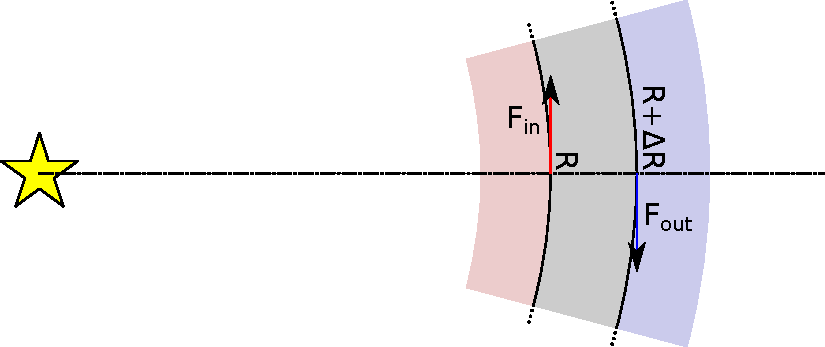
\includegraphics[width=0.7\linewidth]{figure/disk_ring.pdf}
\caption[Bilan de moment cinétique d'un anneau d'épaisseur $\Delta R$.]{Représentation d'un anneau de largeur $\Delta R$ et du
bilan de moment cinétique de ce dernier.}\label{fig:disk_ring}
\end{figure}

On cherche dans un premier temps à faire le bilan de masse de l'anneau considéré. Sa masse s'écrit :
\begin{align}
m_a &= 2\pi R \Delta R \Sigma(R)\label{eq:m_a}
\end{align}

\bigskip

Soit $v_r\hat{e}_r$ la vitesse radiale du gaz (avec $v_r<0$ dans notre cas). Cette vitesse est responsable d'un certain taux d'accrétion du gaz du disque sur l'étoile centrale. On cherche maintenant à modéliser cette accrétion pour le bilan de moment cinétique sur l'anneau.

Pour cela, on cherche à exprimer la variation de masse de l'anneau, ainsi que le moment cinétique emporté par cette variation de masse. 

Au bord interne $R$, par unité de temps, la masse entrant ou sortant de l'anneau peut-être exprimée comme un flux :
\begin{align}
\dif F_M &= \Sigma \cdot 2\pi r \cdot \left( -\vect{v_r} \cdot \vect{\dif S} \right)
\end{align}
En effet, en multipliant la circonférence de l'anneau par la vitesse, on obtient une sorte de surface par unité de temps qui représente ce qui sort de la frontière virtuelle représentée par l'anneau en $r=R$. 

Le flux de matière doit être négatif si la masse sort de l'anneau. Les éléments de surface étant orientés vers l'extérieur, un vecteur vitesse colinéaire à $\vect{\dif S}$ implique que la matière sort de l'anneau. Ceci explique la présence du signe négatif dans l'expression du flux de matière.

On a ainsi aux deux bords de l'anneau :
\begin{subequations}
\begin{align}
\dif F_M(R) &= \Sigma(R) \cdot 2\pi R \cdot v_r(R)\\
\dif F_M(R+\Delta R) &= - 2\pi (R+\Delta R) \cdot v_r(R+\Delta R) \cdot \Sigma(R+\Delta R)
\end{align}\label{eq:dif_F_M}
\end{subequations}
$v_r$ étant négatif, on a bien une perte de masse en $r=R$ et un gain de masse en $r=R+\Delta R$.

La conservation de la masse implique alors que la dérivée temporelle de la masse de l'anneau est égale au flux de masse à travers sa surface. On a ainsi : 
\begin{align*}
\dpd{}{t}\left(2\pi R \Delta R \Sigma(R)\right) &= \dif F_M(R) + \dif F_M(R+\Delta R)
\end{align*}

En faisant tendre l'épaisseur $\Delta R$ de l'anneau vers 0, on obtient alors :
\begin{important}
\begin{align}
\dpd{\Sigma}{t} + \inv{R}\dpd{}{r}\left(R v_r \Sigma\right)&=0\label{eq:conservation_masse}
\end{align}
\end{important}

\subsubsection{Bilan de moment cinétique/angulaire}
On fait maintenant un bilan des variations de moment cinétique pour l'anneau de gaz. Pour cela on dit que la variation de moment cinétique (que l'on écrit en dérivant $J_a(t)$) est égale aux variations de moment cinétiques induites aux bords de l'anneau par échange de masse à laquelle s'ajoute la différence entre les deux couples visqueux qui s'appliquent au bord externe et interne. Ce qui donne : 
\begin{align}
\dod{J_a}{t} &= \dif J(R+\Delta R) + \dif J(R) + \Gamma_\text{out} - \Gamma_\text{in}\label{eq:cons_J_a}
\end{align}

Le moment cinétique de l'anneau est défini par :
\begin{align}
\vect{J_a} &= \vect{R} \wedge (m_a\vect{v(R)}) \nonumber\\
\vect{J_a} &= 2\pi R^3 \Delta R \Sigma(R)\Omega(R)\hat{e}_z\label{eq:J_a}
\end{align}
où $\Sigma$ et $\Omega$ sont la densité de surface et la vitesse angulaire du gaz à la position $R$ dans le disque.

Le flux de moment cinétique est simplement défini comme la quantité de moment cinétique emportée ou apportée par le flux de masse défini précédemment \refeq{eq:dif_F_M} :
\begin{subequations}
\begin{align}
\dif J(R) &= 2\pi v_r(R) \Sigma(R)\cdot R^3\Omega(R)\hat{e}_z\label{eq:dJ_in}\\
\dif J(R+\Delta R) &= -2\pi v_r(R+\Delta R) \Sigma(R+\Delta R)\cdot \left(R+\Delta R\right)^3\Omega(R+\Delta R)\hat{e}_z\label{eq:dJ_out}
\end{align}\label{eq:dJ}
\end{subequations}

\bigskip

À ceci s'ajoute la variation de moment cinétique induite par la friction entre anneaux concentriques, en d'autres termes, dus à la viscosité du disque. Cette variation de moment cinétique est représentée sous la forme d'un couple exercé par les anneaux internes et externes à celui considéré. 

La force visqueuse par unité de longueur est définie par :
\begin{align}
\dif F_\text{vis} &= \nu \Sigma A = \nu \Sigma r \dod{\Omega}{r}
\end{align}
où $A=r \dod{\Omega}{r}$ est le taux de cisaillement.

La force visqueuse induite par les anneaux entourant l'anneau considéré est alors : 
\begin{subequations}
\begin{align}
\vect{F_\text{in}}(R)&= 2\pi\nu \Sigma R^2 \dod{\Omega}{r}(R) \hat{e}_\theta\\
\vect{F_\text{out}}(R+\Delta R)&= 2\pi\nu \Sigma (R+\Delta R)^2 \dod{\Omega}{r}(R+\Delta R) \cdot \hat{e}_\theta
\end{align}
\end{subequations}
L'anneau interne tournant plus vite, la force est dirigée dans le sens de rotation $\hat{e}_\theta$. À l'inverse, l'anneau externe tourne moins vite, il tend à freiner l'anneau de référence et s'oppose à son mouvement. La force est donc opposée au sens de rotation.

\bigskip

Ainsi, le couple $\vect{\Gamma}=\vect{r}\wedge\vect{F}$ issu de chacun des anneaux entourant celui de référence s'écrit :
\begin{subequations}
\begin{align}
\vect{\Gamma_\text{in}} &= 2\pi\nu \Sigma R^3 \dod{\Omega}{r}(R) \hat{e}_z\label{eq:G_in}\\
\vect{\Gamma_\text{out}} &= 2\pi\nu \Sigma (R+\Delta R)^3 \dod{\Omega}{r}(R+\Delta R) \hat{e}_z\label{eq:G_out}
\end{align}\label{eq:J_torques}
\end{subequations}

\bigskip

En utilisant \refeq{eq:J_a}, \refeq{eq:dJ}, \refeq{eq:J_torques}, dans \refeq{eq:cons_J_a} il vient alors :
\begin{align}
\dpd{\Sigma}{t} &= \inv{r}\dpd{}{r}\left\{\inv{\dpd{}{r}\left(r^2\Omega\right)} \dpd{}{r}\left[\nu \Sigma r^3 \left(-\dod{\Omega}{r}\right)\right]\right\}
\end{align}

Dans le cas d'un disque képlerien ($\Omega = \sqrt{\frac{GM}{r^3}}$) on obtient finalement :
\begin{important}
\begin{align}
\dpd{\Sigma}{t} &=\frac{3}{r}\dpd{}{r}\left[\sqrt{r} \dpd{}{r}\left(\nu \Sigma r^\sfrac{1}{2}\right)\right]
\end{align}
\end{important}

Le calcul détaillé est disponible \refsec{app:equation_angular_momentum}.

Cette équation a nécessité les approximations suivantes : 
\begin{enumerate}
\item On suppose que le potentiel gravitationnel est indépendant du temps ($\dod{\Omega}{t}=0$), c'est-à-dire que la masse de l'étoile est constante, l'accrétion ayant un effet négligeable.
\item On suppose que le mouvement du gaz est képlerien $\Omega=\sqrt{\frac{GM}{r^3}}$, ce qui n'est pas rigoureusement vrai, la pression du gaz rendant le mouvement légèrement sous-képlerien.
\end{enumerate}

\subsubsection{Temps de vie et dispersion du disque}\label{sec:dispersion}\index{dissipation du disque}

\begin{figure}[htbp]
\centering
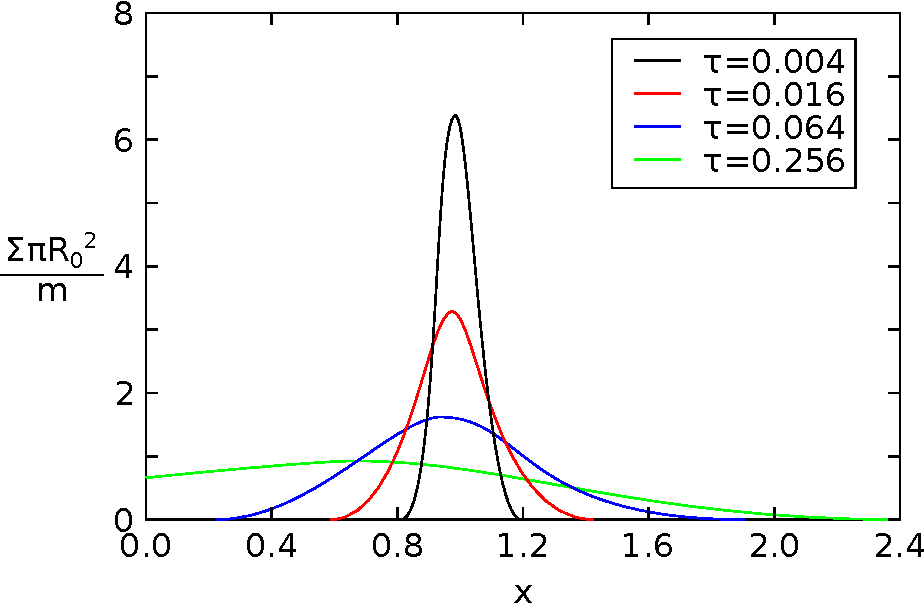
\includegraphics[width=0.65\linewidth]{figure/pringle_viscous_dissipation.pdf}
\caption[Évolution visqueuse d'un anneau de matière]{Évolution visqueuse d'un anneau de matière de masse $m$ et de rayon $R_0$.
La densité de surface est montrée comme une fonction de la longueur dédimensionnée $x=R/R_0$ et du temps adimensionné
$\tau=12\nu t / {R_0}^2$.}\label{fig:pringle_viscous_dissipation}
\end{figure}

Cette équation permet de modéliser l'évolution visqueuse d'un disque au cours du temps. \reffig{fig:pringle_viscous_dissipation}, tirée de \cite{pringle1981accretion} et recalculée illustre l'évolution visqueuse d'un anneau de matière de masse $m$ dans des unités adimensionnées de distance et de temps.

\bigskip

On situe généralement le temps de vie d'un disque protoplanétaire autour de quelques millions d'années. Cette information est obtenue de plusieurs études de d'amas d'étoiles d'âges différents dans lesquelles on mesure le taux d'étoiles possédant un excès infrarouge (signe de présence d'un disque) \citep{williams2011protoplanetary}. 70\% à 80\% des étoiles jeunes ($t<1\unit{Myr}$) possèdent un disque \citep{winston2007combined, gutermuth2008spitzer}, 40 à 50\% des étoiles dans des amas d'âge compris entre 2 et 3 millions d'années en possèdent un \citep{lada2006spitzer, sung2009spitzer} tandis que moins de 20\% des étoiles dans des amas d'environ 5 millions d'années ont un disque \citep{currie2009last}. 

Par la rareté des disques en train de se dissiper, les observations suggèrent aussi que les disques se dissipent très rapidement, avec un temps de dispersion d'environ $10^5$ ans \citep{simon1995disk, wolk1996search}. La dissipation visqueuse n'explique alors pas comment le disque peut subsister pendant plusieurs millions d'années, mais se dissiper complètement en \nombre{500 000} ans. \cite{clarke2001dispersal} ont montré qu'il était possible d'expliquer ce comportement à deux temps caractéristiques à l'aide de la photo-évaporation. 

\begin{figure}[htbp]
\centering
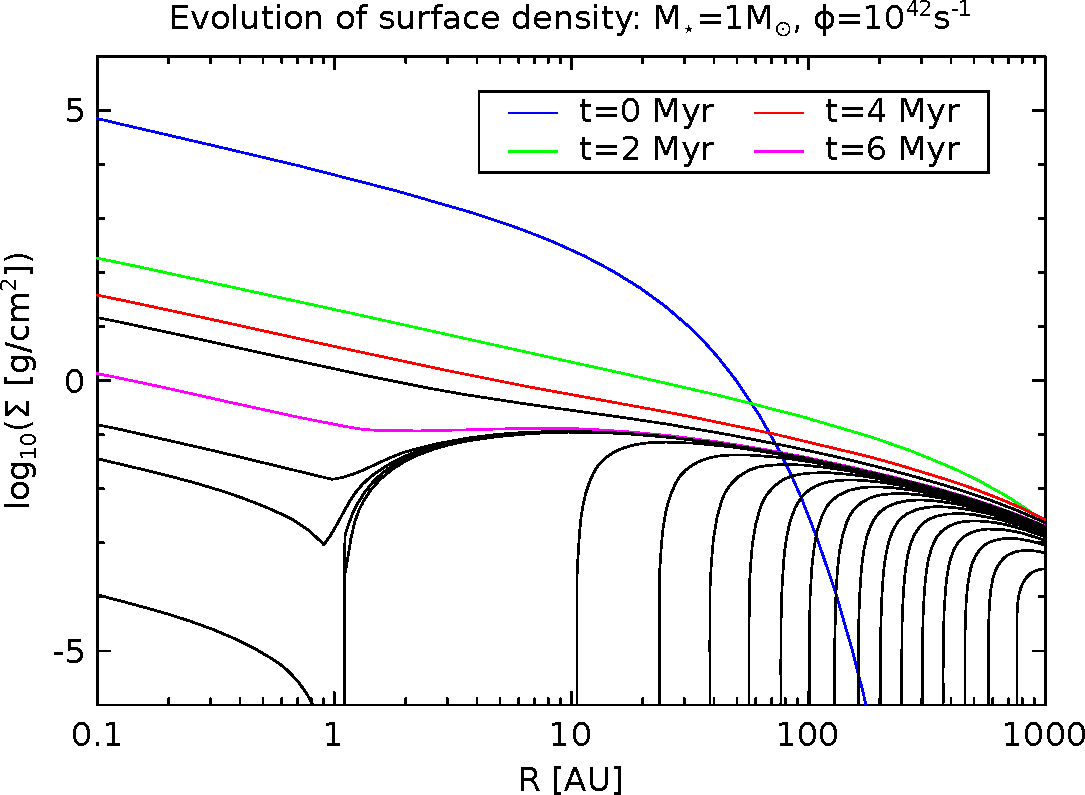
\includegraphics[width=0.65\linewidth]{figure/disk_dispersion.pdf}
\caption[Dissipation du disque]{Évolution de la densité de surface en fonction du temps dans une simulation qui modélise la
dissipation du disque protoplanétaire par évolution visqueuse et photo-évaporation. À $t=6.20\unit{Myr}$ le disque est
totalement dissipé. Figure adaptée de \cite{alexander2006photoevaporation}.}\label{fig:disk_dispersion}
\end{figure}

Le principe de la \gras{photo-évaporation} est que le rayonnement de l'étoile permet de dissocier le dihydrogène ainsi que de fournir de l'énergie cinétique aux atomes du gaz. À partir d'un rayon dit \og rayon gravitationnel\fg $r_g$ qui représente la distance à partir de laquelle l'énergie fournie par les photons de l'étoile devient suffisante pour contrebalancer les effets de sa gravité, la photo-évaporation permet d'évaporer une partie du gaz superficiel du disque. Le disque va alors se creuser jusqu'à séparer le disque en deux. Les parties internes du disques ne sont alors plus alimentées par les parties externes. Des simulations montrent que les parties externes se dispersent rapidement une fois les parties internes accrétées \citep{alexander2006photoevaporation}. \reffig{fig:disk_dispersion} montre l'évolution du profil radial de densité en fonction du temps en présence de l'évolution visqueuse et de la photo-évaporation.

La photo-évaporation est aussi possible par l'irradiation d'étoiles massives (étoiles OB) dans le voisinage du disque \citep{adams2004photoevaporation}.

\subsection{Profil de température}
Du point de vue de la température, il y a principalement deux types de disques : 
\begin{itemize}
\item les \gras[chauffage visqueux]{disques actifs} : la source de température est le disque lui-même, qui par \gras{chauffage visqueux} (frottements) va convertir de l'énergie gravitationnelle en chaleur ;
\item les \gras[irradiation]{disques passifs} : la source de chaleur/température est l'étoile centrale qui éclaire le disque. 
\end{itemize}

Un disque peut à la fois être actif et passif, mais généralement on essaie d'approximer, de considérer que l'un est négligeable devant l'autre. De plus, un disque aura des zones actives et des zones passives, c'est-à-dire que certaines zones seront principalement chauffées par la viscosité alors que d'autres le seront par l'\gras[irradiation]{irradiation de l'étoile}.

\bigskip

Afin de déterminer le profil de température, il faut écrire l'équation de conservation de l'énergie, qui va tenir compte de tous les termes source et toutes les pertes, par unité de surface.

On a tout d'abord les pertes par rayonnement de corps noir. Ensuite, il y a les termes sources. Pour un disque actif, le terme source est le chauffage visqueux. Pour un disque passif, c'est l'irradiation de l'étoile \citep{chiang1997spectral}. Dans notre cas, il y a un terme dû à l'enveloppe du disque, un dû à l'irradiation de l'étoile centrale, et enfin un dernier dû au chauffage visqueux.


\begin{figure}[htbp]
\centering
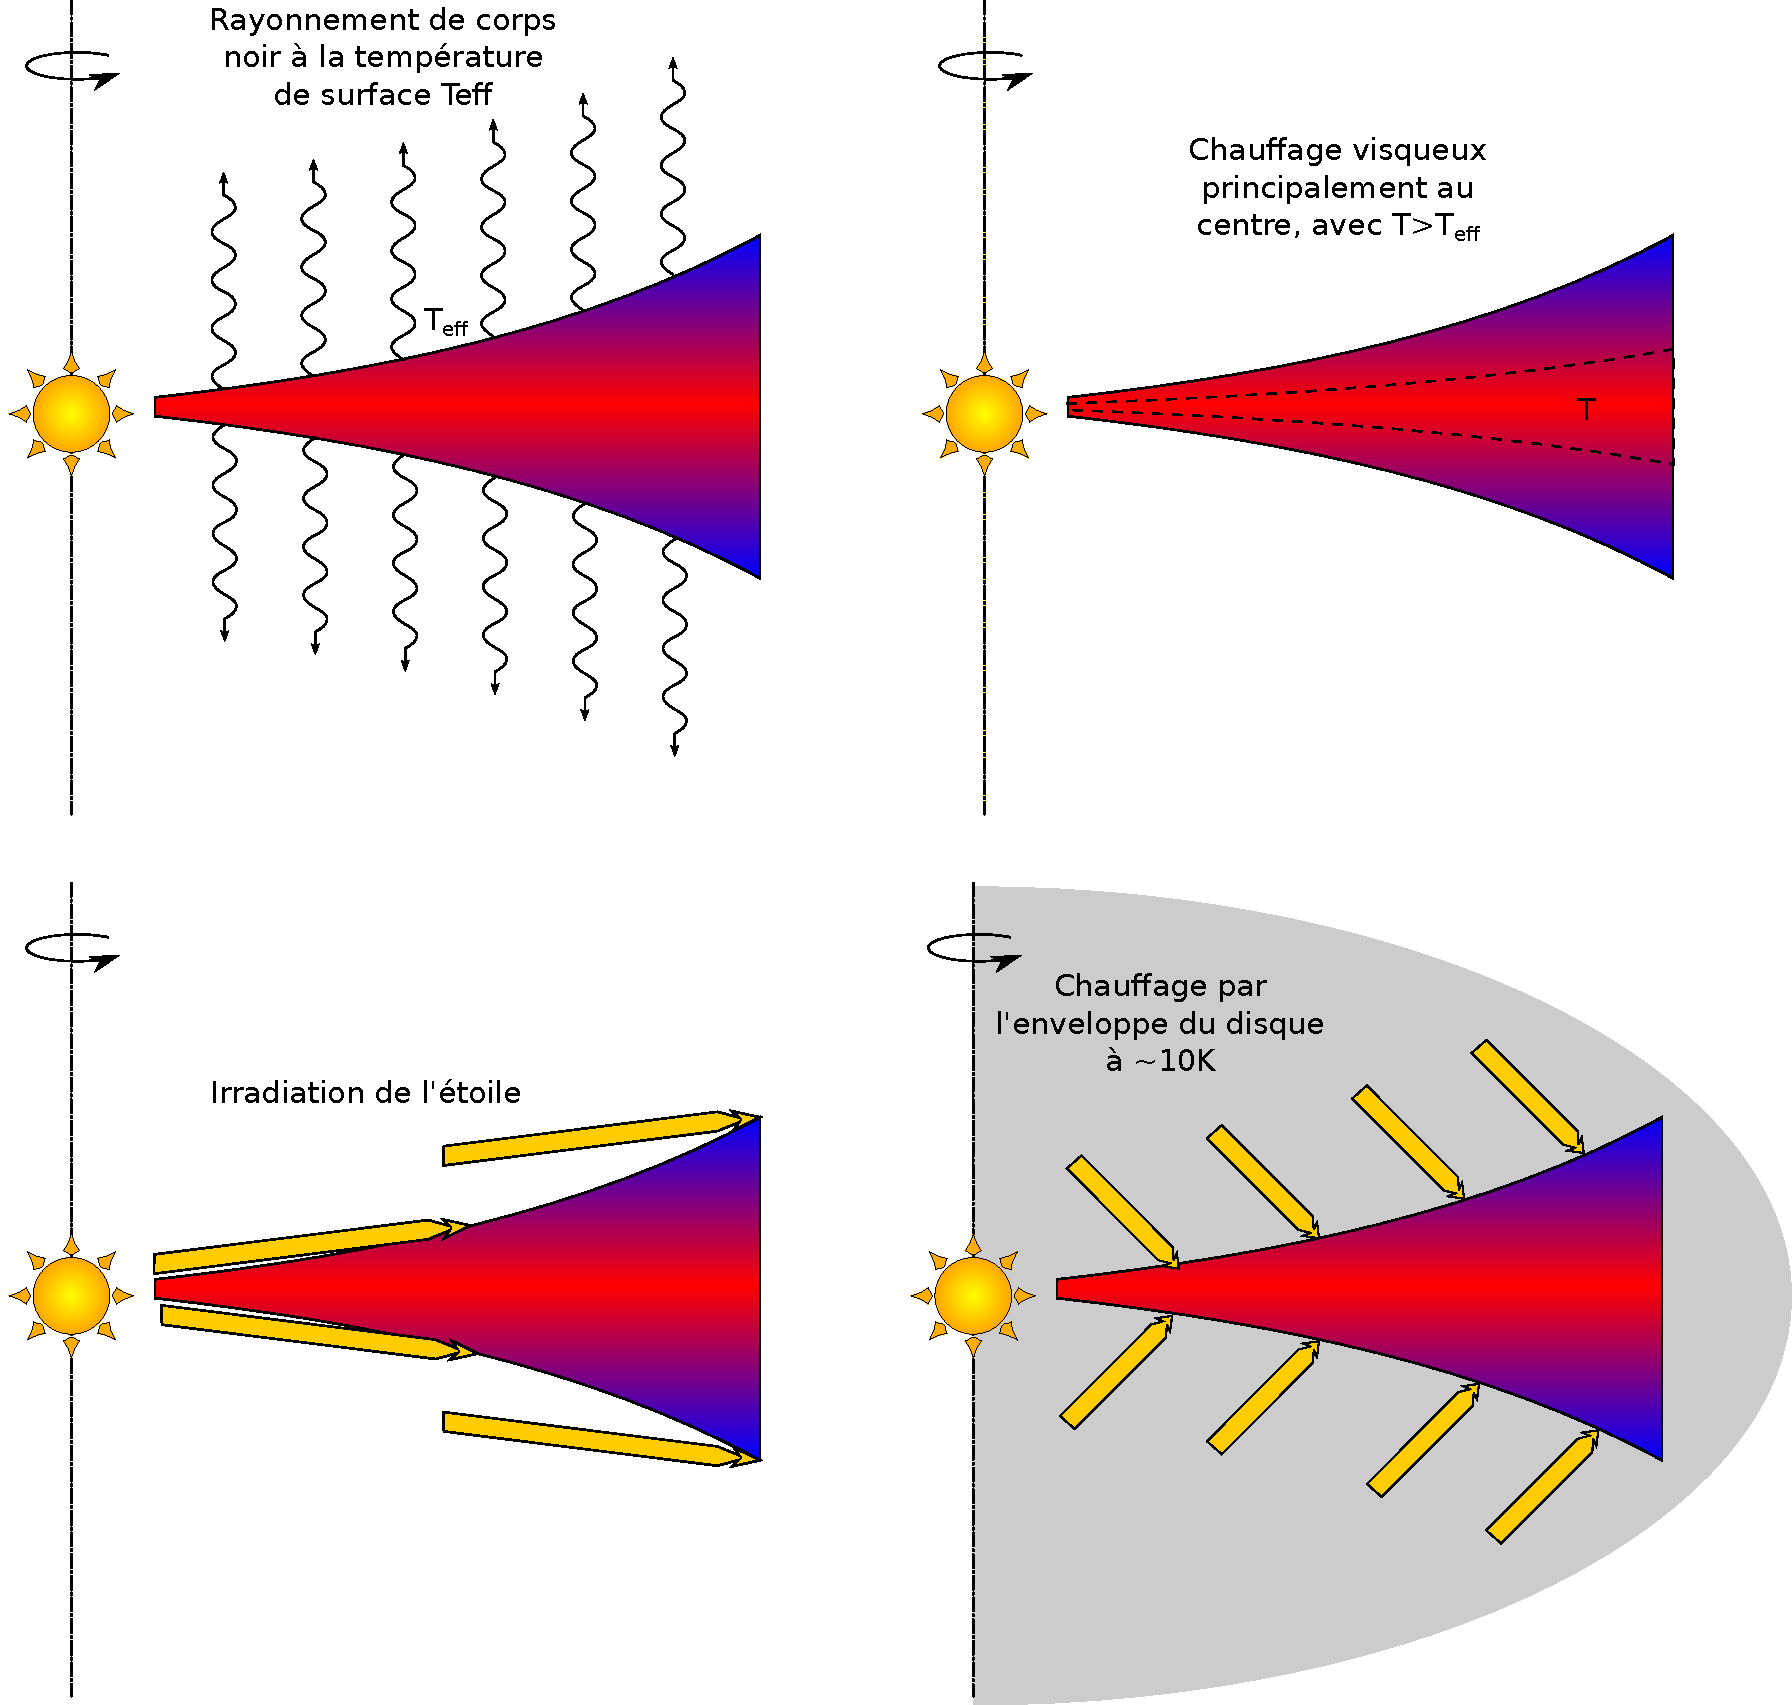
\includegraphics[width=0.65\linewidth]{figure/disk_energy.pdf}
\caption[Bilan énergétique d'un disque.]{Représentation du bilan thermique d'un disque}\label{fig:energy_equilibrium}
\end{figure}

\subsubsection{Refroidissement radiatif}
Par toute la surface du disque, qui est à une température $T_\text{eff}$ en surface, on a des pertes par rayonnement de corps noir : 
\begin{align}
P_\text{cn} &= - 2\sigma {T_\text{eff}}^4
\end{align}
où $\sigma$ est la constante de Stefan-Boltzmann. Ces dernières doivent être multiplié par deux, en effet, il y a des pertes par rayonnements des deux cotés du disque à une position donnée. 

\bigskip

$T_\text{eff}$ est une estimation de la température effective du disque à sa surface \cite{hubeny1990vertical} : 
\begin{subequations}
\begin{align}
{T_\text{eff}}^4 &= \frac{T^4}{\tau_\text{eff}}
\intertext{avec}
\tau_\text{eff} &= \frac{3}{8}\tau + \frac{\sqrt{3}}{4} + \inv{4\tau}
\end{align}
\end{subequations}
où $\tau=\kappa\Sigma/2$ est la profondeur optique verticale moyenne, $\kappa$ étant l'opacité du disque (l'opacité sera détaillée dans \refsec{sec:opacity}).

Cette température effective est le résultat d'un transfert de rayonnement depuis le cœur du disque, à une température $T$ qui se refroidit, et chauffe les différentes couches successives jusqu'à atteindre le bord du disque. Il résulte alors une température $T_\text{eff}$ plus faible que la température dans le plan du disque. 

\subsubsection{Chauffage par l'enveloppe}
\begin{figure}[htbp]
\centering
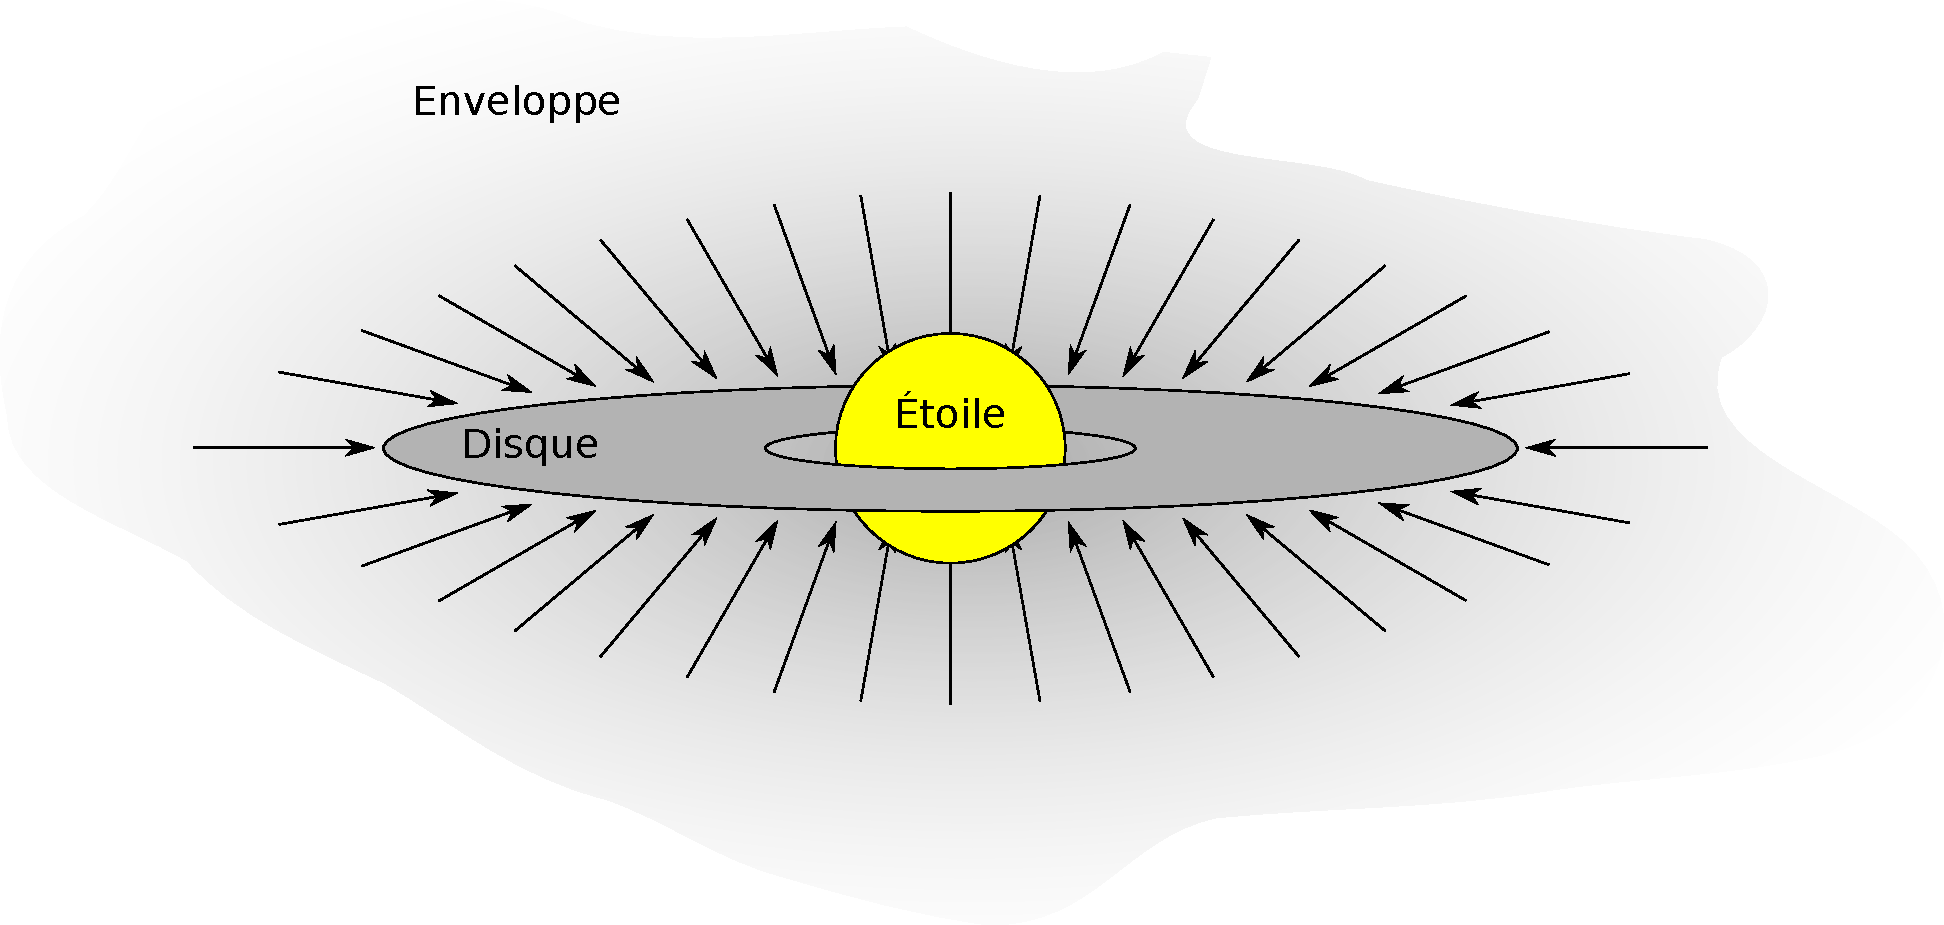
\includegraphics[width=0.65\linewidth]{figure/disk_envelope.pdf}
\caption[Chauffage du disque par l'enveloppe]{Représentation de l'effondrement d'un nuage moléculaire et des différentes parties
qui composent le système en effondrement.}\label{fig:envelope}
\end{figure}
L'enveloppe \reffig{fig:envelope} provient de l'effondrement continu du nuage moléculaire. C'est un reste diffus qui alimente continuellement le disque en matière. Mais cette enveloppe, qui possède une température que l'on fixe ici à $T_\text{en} = 10\unit{K}$ contribue aussi au bilan d'énergie du disque en apportant la contribution uniforme suivante :
\begin{align}
C_\text{en} &= 2 \sigma {T_\text{en}}^4
\end{align}

La température de l'enveloppe étant très faible, cette dernière ne contribue que dans les parties externes du disque, là où la densité de surface du gaz est très faible, rendant du même coup le chauffage visqueux extrêmement ténu lui aussi.

\subsubsection{Chauffage par l'étoile}\label{sec:irradiation}\index{irradiation}
La surface du disque reçoit de la lumière de l'étoile centrale. Soit $R_\star$, $L_\star$ respectivement le rayon et la luminosité de l'étoile. Soit $\varepsilon$ l'albédo du disque, que l'on choisi typiquement égal à $0.5$  \citep{menou2004low}. 

Le flux incident est alors \citep[eq. (7)]{menou2004low} : 
\begin{align}
F_\text{irr} &= \frac{L_\star(1-\varepsilon)}{4\pi r^2} \alpha
\end{align}
où $\alpha$ (avec $\alpha\ll 1$) représente l'angle entre les rayons incidents et la surface du disque. 

D'après notamment \cite[eq. (5)]{chiang1997spectral}, cet angle peut être écrit comme : 
\begin{align}
\alpha &= 0.4 \frac{R_\star}{r} + r \dod{}{r}\left(\frac{H}{r}\right)
\end{align}

On note que dans cette expression, le premier terme illustre le fait que l'étoile n'est pas ponctuelle, et que ceci a un effet sur l'irradiation dès que l'on s'approche de cette dernière. Le deuxième terme représente la surface du disque qui intercepte le rayonnement incident, et qui est fonction de la variation d'échelle de hauteur du disque (plus le disque est évasé, et plus la paroi qui intercepte le rayonnement est abrupte). 

Il vient enfin, en exprimant la luminosité de l'étoile en fonction de sa température et de son rayon, l'expression suivante :
\begin{align}
C_\text{irr} &= 2 \sigma {T_\star}^4 \frac{{R_\star}^2}{r^2} (1-\varepsilon) * \left[0.4 \frac{R_\star}{r} + r \dod{}{r}\left(\frac{H}{r}\right)\right]
\end{align}

Il faut cependant noter qu'une approximation implicite a été faite, c'est de dire que $h_p\sim h$, où $h_p$ est la position verticale dans le disque où les photons stellaires sont absorbés. En effet, l'absorption des photons ne dépend pas simplement de la densité, mais aussi de l'opacité du disque aux photons stellaires, qui dépend de la composition du disque.

Dans le cadre d'un disque optiquement épais, il devient possible de considérer $h_p \sim h$.

%non ponctualité de l'étoile : Chiang & Goldreich, 1997, ApJ, 490, 368
%expression de l'angle notammenet : dullemond 2000
%autres expressions : menou & goodman 2004

\subsubsection{Chauffage visqueux}\index{chauffage visqueux}
On considère un fluide incompressible. Il peut paraître étonnant de considérer un disque de gaz comme étant un fluide incompressible. Mais en fait l'aspect compressible va surtout se manifester lors de la mise à l'équilibre, générant des ondes de chocs par exemple. Mais une fois le disque stabilisé tout se passe comme si on avait un fluide incompressible. C'est matérialisé par le fait que la vitesse dans le disque est considérée comme inférieure à la vitesse du son dans le milieu $c_s$, au delà de laquelle on aura des ondes des choc ayant une incidence sur le bilan thermique. Ainsi donc, en considérant un fluide incompressible, on peut partir de l'expression de la variation d'énergie cinétique (qui est l'inverse du chauffage, les pertes cinétiques étant converties en chaleur par la viscosité) \citep[(16.3)]{landau1989mecanique} : 
\begin{align}
\dpd{E_c}{t} &= - \frac{1}{2}\int \eta(T_{ik})^2\dif V\\
T_{ik} &= \left(\dpd{v_i}{x_k} + \dpd{v_k}{x_i}\right)\nonumber
\end{align}
où $\eta = \rho\nu$ est la viscosité dynamique\footnote{$\nu$ étant la viscosité cinématique et $\rho$ la densité volumique de gaz.}

À partir de \citep[(15.8) et (15.17)]{landau1989mecanique}, on extrait de manière assez directe l'expression du tenseur $T_{ik}$ en coordonnées cylindriques : 
\begin{align}
T_{rr} &= 2\dpd{v_r}{r}, & T_{r\varphi} &= \left(\inv{r} \dpd{v_r}{\varphi} + \dpd{v_\varphi}{r} - \frac{v_\varphi}{r}\right),\nonumber\\
T_{\varphi\varphi} &= 2 \left(\inv{r} \dpd{v_\varphi}{\varphi} + \frac{v_r}{r}\right), & T_{\varphi z} &= \left(\dpd{v_\varphi}{z} + \inv{r}\dpd{v_z}{\varphi}\right),\\
T_{zz} &= 2\dpd{v_z}{z}, & T_{rz} &= \left(\dpd{v_z}{r} + \dpd{v_r}{z}\right).\nonumber
\end{align}
sachant que le tenseur est symétrique en statique, ce qui donne : 
\begin{align}
T_{ik} &= \begin{pmatrix}
T_{rr} & T_{r\varphi} & T_{rz}\\
T_{r\varphi} & T_{rr} & T_{\varphi z}\\
T_{rz} & T_{\varphi z} & T_{zz}
\end{pmatrix}
\end{align}

À partir de ces expressions, nous allons procéder à quelques simplifications, moyennant quelques approximations : 
\begin{itemize}
\item On considère tout d'abord que $v_z=0$ en invoquant le fait que le disque est à l'équilibre hydrostatique verticalement. 

\item Ensuite, on néglige tous les termes en $\pd{}{\varphi}$ car le disque est axisymétrique. 

\item On néglige enfin tous les termes en $v_r$ devant les termes en $v_\varphi$ étant donné que la vitesse de dérive (liée à l'accrétion) est beaucoup plus petite que la vitesse de rotation due au mouvement képlerien. En effet, la vitesse de dérive est une conséquence des pertes d'énergie par frottement visqueux entre deux anneaux due à la différence de vitesse de leur mouvement képlerien.
\end{itemize}

Seul le terme $T_{r\varphi}$ reste :
\begin{align}
T_{r\varphi} &= \dpd{v_\varphi}{r} - \frac{v_\varphi}{r}\nonumber\\
\intertext{avec $v_\varphi=r\Omega$}
T_{r\varphi} &= r\dod{\Omega}{r}
\end{align}

Il vient alors :
\begin{align*}
\dpd{E_c}{t} &= - \frac{1}{2}\int \eta(T_{ik})^2\dif V\\
&= - \frac{1}{2}\int \eta\sum_{i=1}^3\sum_{j=1}^3 {T_{ij}}^2\dif V\\
&= - \frac{1}{2}\int \eta\left({T_{r\varphi}}^2+{T_{\varphi r}}^2\right)\dif V\\
\intertext{Le tenseur est symétrique, on a donc $T_{r\varphi} = T_{\varphi r}$}
&= - \frac{1}{2}\int \eta\left(2{T_{r\varphi}}^2\right)\dif V\\
&= - \iint \rho\nu \left(r\dod{\Omega}{r}\right)^2\dif S\dif z\\
\intertext{En utilisant une vitesse angulaire képlerienne $\Omega=\sqrt{\frac{GM}{r^3}}$ on obtient alors :}
&= - \int \Sigma\nu \left(-\frac{3}{2}\Omega\right)^2\dif S\\
\dpd{E_c}{t} &= - \frac{9}{4} \int \Sigma\nu \Omega^2\dif S
\end{align*}

La variation d'énergie cinétique est négative, cette perte est convertie en chaleur par chauffage visqueux. Le chauffage visqueux intégré sur toute la surface du disque peut ainsi être défini comme : 
\begin{align*}
C_\text{vis/tot} &= - \dpd{E_c}{t}
\end{align*}
de sorte qu'on peut écrire le chauffage visqueux par unité de surface comme étant égal à :
\begin{align}
C_\text{vis} &= \frac{9}{4} \nu\Sigma\Omega^2
\end{align}

\subsubsection{Bilan}
On cherche maintenant la température d'équilibre du disque, compte tenu de tous les termes rentrant dans l'équation bilan de l'énergie du disque. Il vient alors, en considérant le chauffage visqueux, l'irradiation de l'étoile centrale, le chauffage par l'enveloppe et les pertes par radiation à la surface du disque : 
\begin{align}
0 &= P_\text{cn} + C_\text{en} + C_\text{irr} + C_\text{vis}\nonumber\\
0 &= - 2\sigma \frac{T^4}{\frac{3}{8}\tau + \frac{\sqrt{3}}{4} + \inv{4\tau}} + 2 \sigma {T_\text{en}}^4 + 2 \sigma {T_\star}^4 \frac{{R_\star}^2}{r^2} (1-\varepsilon) * \left[0.4 \frac{R_\star}{r} + r \dod{}{r}\left(\frac{H}{r}\right)\right] + \frac{9}{4} \nu\Sigma\Omega^2\label{eq:equation_energie}
\end{align}

Dans la pratique, c'est une équation de l'on résout de manière numérique, par itération. En effet, beaucoup de paramètres dépendent de la température, alors même que c'est la variable que l'on recherche. 

Ce calcul est lui-même extrêmement dépendant de la définition que l'on choisi pour l'opacité $\kappa$ et de la dépendance de cette dernière en fonction de la température, la densité ou la pression. 

\subsection{La viscosité du disque}\label{sec:viscosite}\index{viscosité}% (Franck et al. 1992)
La viscosité moléculaire, viscosité généralement considérée quand on étudie la dynamique d'un fluide, peut être définie par : 
\begin{align}
\nu_m &\sim \lambda c_s
\end{align}
où $c_s$ est la vitesse du son dans le milieu et $\lambda$, libre parcours moyen dans le gaz avec une concentration de particule $n$ est :
\begin{align}
\lambda &= \inv{n\sigma_\text{mol}}
\end{align}

On cherche ici à faire un calcul d'ordre de grandeur, on ne se préoccupe pas des détails plus fins qui seraient normalement nécessaires pour calculer une viscosité moléculaire. 

On prend pour section efficace de collisions celle de l'hydrogène moléculaire \citep{chapman1970mathematical} :
\begin{align}
\sigma_\text{mol} &= 2\times 10^{-15}\unit{cm^2}
\end{align}

On considère ensuite un disque dont la densité de surface $\Sigma$ à $1\unit{UA}$ vaut $\Sigma_0 = 500\unit{g/cm^2}$. En utilisant \refeq{eq:surface-to-volume} on a alors $\rho=2.67\cdot 10^{-10}\unit{g/cm^{-3}}$. Il vient la concentration $n=6.8\cdot 10^{13}\unit{cm^{-3}}$. On obtient alors une viscosité moléculaire à $1\unit{UA}$ de l'ordre de : 
\begin{align}
\nu_m &\sim 1.0\times 10^6\unit{cm^2/s}
\end{align}

Le temps caractéristique de l'évolution visqueuse qui en découle est alors : 
\begin{align}
t_\nu &\simeq \frac{r^2}{\nu_m} &= 6.5\times 10^{12}\unit{ans}
\end{align}
c'est-à-dire plus d'un million de fois le temps de vie observé des disques protoplanétaires qui se situe autour du million d'années \citep{williams2011protoplanetary}.

En conséquence, quand on parle de viscosité $\nu$\footnote{Viscosité cinématique} dans un disque, ce n'est pas la viscosité moléculaire classique, bien trop faible aux densités rencontrées. On suppose généralement une viscosité due à la turbulence qui est beaucoup plus importante que la viscosité moléculaire, mais qui peut être traitée par les mêmes équations. 

%TODO Et calculer le taux d'accrétion (3 pi nu sigma) et comparer aux valeurs typiques de 1e-8 masses solaires par an. Je n'ai pas compris cette partie, du coup j'ai plutôt fait le temps d'évolution visqueux par rapport au temps de vie des disques observés.

Il est rare que la viscosité soit calculée de manière cohérente. L'importante augmentation du temps de calcul n'apporterait pas forcément beaucoup plus de précisions étant donné les nombreuses incertitudes sur la poussière, le couplage et le champ magnétique. 

\bigskip

La première hypothèse est de considérer une viscosité constante. Ce n'est certainement pas satisfaisant, sûrement éloigné de la vérité, mais on a ainsi un seul paramètre et on n'ajoute pas de surcouche de complexité apportant son lot supplémentaire d'incertitude. Reste qu'une viscosité constante dans un disque très étendu, par exemple allant de $0.1\unit{UA}$ à $100\unit{UA}$ n'est certainement pas cohérent avec la physique du disque. 

Un autre modèle très répandu pour la viscosité du disque est la prescription $\alpha$.

\subsubsection{Les disques alpha}\label{sec:viscosite-alpha}\index{prescription alpha}
On peut introduire un paramètre adimensionné $\alpha$ \citep{shakura1973black}. Dans ce formalisme, plusieurs hypothèses sont faites : 
\begin{itemize}
\item On considère que la turbulence est subsonique.
\item L'échelle des tourbillons des turbulences est plus petite que l'échelle de hauteur du disque
\end{itemize}
Le mécanisme qui a le plus de chance d'être à l'origine de la viscosité alpha est l'\gras{Instabilité Magnéto-Rotationnelle} (MRI) \citep{balbus1991powerful}. 

\bigskip

En conséquence, on peut définir la viscosité $\nu$ associée à la turbulence comme étant 
\begin{align}
\nu &= \alpha c_s H
\end{align}
où $c_s$ est la vitesse du son et $H$ l'échelle de hauteur du disque. $\alpha$ (avec $\alpha \ll 1$) est alors un paramètre adimensionné qui permet de définir plus ou moins l'intensité des turbulences, et donc la viscosité qui leur est associée. Une valeur typique d'$\alpha$ se situe entre $10^{-2}$ et $10^{-4}$ \citep{guilloteau2011dual}.

Ce modèle permet de définir une viscosité non-constante dans le disque de gaz ce qui semble déjà plus cohérent avec un disque de gaz étendu ($[0.1-100]\unit{UA}$ par exemple). 

Pourtant, le modèle $\alpha$ n'est pas forcément la panacée en comparaison du modèle à viscosité constante. En effet, la complexité est ici masquée dans la valeur qu'il faut attribuer au paramètre $\alpha$. D'une part il est difficile d'estimer la valeur du paramètre $\alpha$ mais en plus il n'y a aucune raison physique qui permet de justifier qu'$\alpha$ soit constant dans tout le disque (approximation généralement sous-jacente au choix de la prescription $\alpha$ pour la viscosité).

Ceci justifie donc que l'on mette ces deux modèles en concurrence, sans placer le modèle $\alpha$ au dessus du modèle à viscosité constante. Les incertitudes étant tellement grandes dans les deux cas, il est justifié d'explorer ces deux modèles et de les comparer quand cela nous est donné de le faire.

\subsubsection{Ionisation et zones mortes}\label{sec:ionisation_DZ}\index{ionisation}\index{zone morte}
Pour que la MRI se développe, c'est-à-dire qu'il y ait un couplage entre le champ magnétique et les mouvements du disque, il faut qu'une partie au moins du disque soit ionisé. Dans ces régions ionisées, on pourra alors avoir transport du moment cinétique via la viscosité turbulente. 

\bigskip

Sans ionisation, il n'y a pas de couplage entre le champ magnétique et la matière, et donc pas de turbulence induite par ce même champ. \index{ionisation}

\reffig{fig:ionization} représente les différents processus d'ionisation dominants en fonction de la zone du disque considérée.
Mais si le taux d'ionisation décroit en fonction de la distance orbitale \citep{ilgner2006ionisation1} comme le montre
\reffig{fig:ilgner_ionisation}, il en va de même avec la densité de surface du disque. Il est donc probable que certaines zones
du disque ne soient pas ionisées (en pourcentage du nombre total d'atomes disponibles), et donc que le transport du moment
cinétique s'y fasse peu ou pas du tout \citep{gammie1996layered}. Ces zones, appelées \gras{zone morte} (ou \og dead zone\fg en anglais), sont donc des zones où
la turbulence est faible ou inexistante, et où la viscosité est par conséquent beaucoup plus faible. 

\begin{figure}[htbp]
\centering
\subfloat[Mécanisme principal d'ionisation de différentes zones du disque. Les zones où l'ionisation est très faible, appelées zones mortes sont des positions où on pense que la viscosité turbulente est extrêmement faible.]{\label{fig:ionization}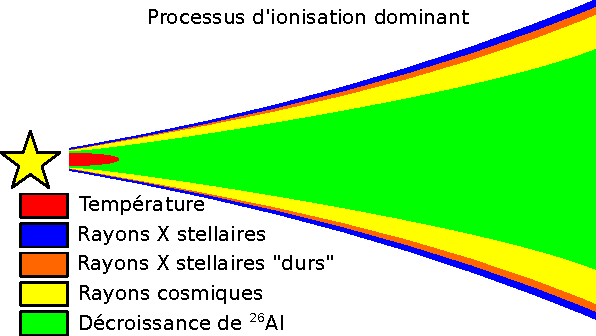
\includegraphics[width=0.49\textwidth]{figure/disk_ionization.pdf}}\hfill
\subfloat[Taux effectif d'ionisation $\zeta_\text{eff}$ par atome d'hydrogène pour un disque avec $\alpha=10^{-2}$ et $\dot{M}=10^{-7}\unit{M_\odot yr^{-1}}$. Les lignes de référence correspondent aux valeurs de $\zeta_\text{eff}$ suivante : $10^{-19}$, $10^{-21}$ et $10^{-23}\unit{s^{-1}}$. Cette figure est basée sur la figure 6 de \cite{ilgner2006ionisation1}.]{\label{fig:ilgner_ionisation}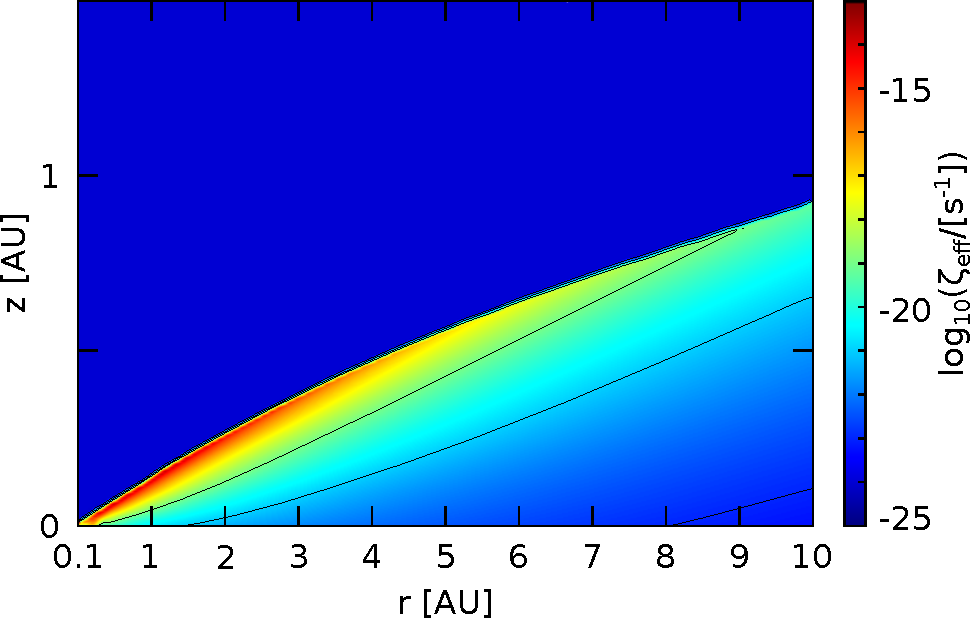
\includegraphics[width=0.49\textwidth]{figure/ilgner_ionization_rate.pdf}}
\caption[Ionisation dans un disque protoplanétaire]{Représentation de l'ionisation dans un disque protoplanétaire}
\end{figure}

On voit donc que les modèles de viscosité constante ou alpha sont incapables de rendre compte de la présence de ces zones de manière intrinsèque. Il est possible de modifier artificiellement les profils de viscosité pour faire apparaître de telles zones mais ça reste \emph{ad hoc}. Dans la suite, je n'ai pas modélisé de zone morte même s'il est probable qu'elles aient un effet sur la migration, le modèle sans zone morte n'est encore pas suffisamment bien compris pour que le rajout de ces zones sans ionisations soit pertinent.

\subsection{La poussière}\index{poussière}
Le disque protoplanétaire est principalement composé de gaz, hydrogène et hélium en majorité. Pourtant, même si la poussière ne représente qu'environ 1\% de la masse du disque elle joue un rôle au moins aussi important que le gaz lui-même.

À cause de la pression quasi-inexistante dans le disque en raison des faibles densités, solide et gaz sont les seules phases existantes, il n'y a pas de liquides dans l'espace. La poussière représente la matière solide du disque, en grains plus ou moins fin, allant du nanomètre, micromètre, jusqu'à des tailles planétaires en fin de formation. 

Cette poussière est un composé extrêmement complexe à modéliser. Elle contient différents composés solides en fonction de la température (à certaines températures et densité des composés se volatilisent et d'autres non). La ligne des glaces représente la distance à partir de laquelle de la glace d'eau apparait, augmentant de manière drastique la quantité de poussière dans le disque. 

Le disque évoluant au cours du temps, la ligne des glace évolue elle aussi à mesure que les propriétés du disque, et en particulier son profil de densité de gaz change \citep{dodsonrobinson2009icelines}.

\bigskip

De plus, la poussière est aussi responsable de l'opacité du disque, c'est-à-dire sa capacité à laisser passer ou non la lumière. À travers l'opacité, la poussière a donc une influence sur la température du disque qui se refroidit plus ou moins efficacement, et qui absorbe le rayonnement stellaire plus ou moins efficacement. 

\subsection{Opacité du disque}\label{sec:opacity}\index{opacité}
Un paramètre crucial des modèles de disques protoplanétaires est l'opacité du disque qui représente l'absorption du rayonnement incident par une cellule de gaz. Cette dernière dépend principalement de la composition chimique de la poussière sauf quand la température devient suffisamment importante pour que la totalité de la poussière se sublime, généralement au delà de $1500\unit{K}$ \citep{pollack1994composition}, l'opacité étant alors régie par les molécules du gaz.

En fonction de la température et de la pression, différentes espèces se condensent ou se subliment, modifiant les propriétés de la poussière (notamment la quantité de poussière disponible) et donc l'opacité.

L'opacité dépend de plus de la longueur d'onde, les raies d'absorptions n'étant pas uniformément réparties sur toute la gamme de longueur d'onde. Ce dernier paramètre est généralement intégré dans des modèles d'opacité. Citons notamment les opacités moyennes de Planck et de Rosseland, principales opacités utilisées dans les disques. Ce sont des quantités moyennées sur tout un spectre, rendant les opacités indépendantes de la longueur d'onde. 

Dans le cas de l'opacité de la moyenne de Rosseland, on fait l'approximation que le disque est optiquement épais, de sorte qu'on puisse négliger le flux total pour se concentrer uniquement sur la dérivée du flux. c'est-à-dire, en d'autres termes, que seul le flux provenant du gaz environnant arrive jusqu'à la zone considérée, le reste étant absorbé. Dû à l'aspect optiquement épais du disque, on perd l'information sur le flux total, ce qui simplifie les calculs. L'opacité moyenne de Rosseland $\moy{\kappa_R}$ est alors définie comme : 
\begin{align}
\inv{\moy{\kappa_R}} &= \inv{\int_0^\infty \pd{B_\nu}{T}\dif \nu} \int_0^\infty \frac{\pd{B_\nu}{T}}{\kappa_\nu}\dif \nu
\end{align}
où $B_\nu$ et $\kappa_\nu$ sont l'intensité et l'opacité spécifique (dépendant de la fréquence).

À l'inverse, les opacités de Planck concernent les disques optiquement minces, où on ne peut plus considérer uniquement la dérivée du flux. La moyenne est alors effectuée sur l'intensité spécifique directement : 
\begin{align}
\inv{\moy{\kappa_P}} &= \inv{\int_0^\infty B_\nu\dif \nu} \int_0^\infty \frac{B_\nu}{\kappa_\nu}\dif \nu
\end{align}
où $\int_0^\infty B_\nu\dif \nu$ représente l'intensité totale, tandis que $B_\nu$ et $\kappa_\nu$ sont l'intensité et l'opacité spécifique (dépendant de la fréquence).

Dans la pratique, on fait bien souvent l'approximation que le disque est optiquement épais, ce qui est généralement vrai dans les parties internes du disque ($0.1-15\unit{UA}$), lieu de formation des planètes. Pour autant, le calcul des opacités est loin d'être trivial et plusieurs modèles proposent des tables d'opacités dont le détail des propriétés est différent. Le choix du modèle a donc des implications importantes sur le modèle de formation planétaire comme je le détaillerai dans la partie \refsec{sec:influence_opacity_table}. 

En formation planétaire, le modèle le plus utilisé est \citep{bell1994FU}. Mais dans mes études, j'ai utilisé en tout et pour tout 4 modèles différents \citep{bell1994FU, zhu2009nonsteady, chambers2009analytic, hure2000transition}. À noter que \citep{bell1994FU, zhu2009nonsteady} sont des modèles qui proposent différents fonctions analytiques pour définir une opacité par morceaux. \citep{chambers2009analytic} propose un modèle très simple à opacité constante $\kappa=3$ tant que la température est inférieure à $1380\unit{K}$, puis une simple loi de puissance, fonction uniquement de la température au delà. Enfin, le modèle dans \citep{hure2000transition} ne définit pas de fonctions par morceaux mais utilise simplement une table d'opacité fonction de la température et de la densité. L'avantage de ce type de méthode est qu'on ne rajoute pas d'incertitudes par des ajustements en loi de puissance, c'est donc principalement pour ça que j'ai choisi cette table d'opacité pour mon modèle standard. 

\subsection{Profil de densité de surface}
Un point crucial dans la modélisation physique d'un disque protoplanétaire est son profil de densité de surface $\Sigma$. Ça signifie d'une part qu'on fait l'approximation d'un disque mince, et que toutes les quantités qu'on considère par la suite sont moyennées selon la direction verticale $z$.

Que l'on fasse évoluer la densité de surface ou non, on doit choisir un profil initial. Ce profil est généralement sous forme d'une loi de puissance de la forme : 
\begin{align}
\Sigma(R) &= \Sigma_0 \cdot \left(\frac{R}{R_0}\right)^{-\alpha}
\end{align}

Un profil largement utilisé est celui de la Masse Minimale de la Nébuleuse Solaire\footnote{MMSN : Minimum Mass Solar Nebulae} \citep{weidenschilling1977distribution, hayashi1981structure}. Dans cet article, le profil de densité est calculé à partir de la masse des planètes. La quantité de solide contenu dans les planètes est répartie dans des anneaux en lieu et place des planètes, puis à partir d'un rapport gaz sur poussière, le profil de densité de surface du gaz est calculé, puis approximé par une loi de puissance, ce qui donne : 
\begin{align}
\Sigma(R) &= 1700 \left(\frac{R}{1\unit{UA}}\right)^{-\sfrac{3}{2}} \unit{g/cm^2}
\end{align}
La première chose, c'est que c'est une masse minimale, c'est-à-dire qu'on suppose que toute la masse de poussière présente dans le disque de gaz se retrouve dans la masse finale des planètes, ce qui est hautement improbable, que ce soit à cause notamment de l'accrétion sur l'étoile ou de la disparition d'embryons de planètes soit en tombant dans l'étoile, soit par éjection du système.

Ce profil est malgré tout une base de travail, vu qu'il est extrêmement difficile de déduire ces informations des observations des disques. Malgré tout, les études semblent montrer que l'on s'attend à un profil moins abrupt que $\Sigma\propto r^{-\sfrac{3}{2}}$, plus proche de $\Sigma\propto r^{-1}$ \citep{bell1997structure}.

Mais on voit quand même que l'on a une grande liberté sur la densité de surface du disque, à la fois parce qu'on sait à ce jour peu de chose à ce sujet, mais aussi et surtout parce qu'au cours de son évolution, le disque de gaz va voir sa densité de surface varier énormément. En variant le profil, on étudie donc aussi différentes étapes de formation d'un même disque. 

Le profil de densité de surface, que ce soit au travers de $\Sigma_0$ ou de l'indice $\alpha$ de la loi de puissance a une grande influence sur les autres paramètres du disque, notamment le profil de température, au travers du chauffage visqueux notamment. 

Il est aussi crucial de garder à l'esprit que la loi de puissance n'est qu'un modèle, issu notamment des observations qui sondent les parties externes des disques, au delà de plusieurs dizaines d'unités astronomiques. Extrapoler ces lois de puissances jusqu'aux parties les plus internes est une très grande approximation qui a des conséquences importantes pour les planètes, dont le lieu de formation se situe vraisemblablement dans les parties internes.

\subsection{Limites et approximations dues à la modélisation}
Tout d'abord, le bord interne est une des parties les plus complexes d'un disque protoplanétaire. Ce bord interne correspond à des zones différentes pour le gaz ou pour la poussière. La poussière disparait quand la température du disque dépasse $1500\unit{K}$ environ, température au delà de laquelle la partie réfractaire des grains se sublime. 

Le gaz, quant à lui, ne se propage pas non plus jusqu'à la surface de l'étoile en raison du champ magnétique important autour des jeunes étoiles. Le bord interne est ainsi déterminé par le rayon de corotation de l'étoile, c'est-à-dire la distance à laquelle une particule en rotation képlerienne orbite à la vitesse de rotation de l'étoile. Le champ magnétique de l'étoile tournant à la vitesse de rotation de l'étoile, ce rayon de corotation correspond ainsi au rayon en dessous duquel le gaz est freiné par le champ magnétique et est rapidement accrété le long des lignes de champ. 

\bigskip

En considérant un système \og étoile + disque\fg isolé, il n'y a pas d'arrêt brutal de la distribution de matière au bord externe qui est donc plutôt une limitation numérique nécessaire aux simulations. La réalité est représentée plus fidèlement par une décroissance continue de la matière, difficile à modéliser tant pour le bord externe que pour la distribution azimutale du disque. 

Généralement, on considère donc que la taille verticale du disque est égale à une échelle de hauteur (grandeur caractéristique de la décroissance exponentielle verticale de la densité de matière), tandis que la taille radiale du disque dépend de la physique que l'on considère. Dans mon cas j'ai souvent pris un bord externe à $100\unit{UA}$.

Je vais ici essayer de récapituler les approximations qui ont été faites jusque-là sur la physique des disques, et qui vont se retrouver implicitement dans tout code qui implémente les équations décrites ci-dessus : 
\begin{enumerate}
\item On suppose que les disques évoluent de manière isolée. Les études suggèrent que les étoiles se forment majoritairement dans des amas (clusters) à l'intérieur desquels la plupart des étoiles font partie de systèmes binaires ou multiples \citep{duquennoy1991multiplicity}. Même si cette approximation permet la modélisation de l'évolution du disque, il est probable que des effets de voisinages aient des conséquences dans tout ou partie des systèmes stellaires, en particulier au travers de la photo-évaporation supplémentaire induite par les étoiles du voisinage.
\item On néglige l'auto-gravité du disque ($M_d \lesssim \frac{H}{R}M_\star$) en considérant que la période où ce n'est pas le cas est courte devant le temps de vie du disque, et que ce dernier tend rapidement vers une configuration où l'auto-gravité est négligeable.
\item On considère que le gaz est en rotation képlerienne $\Omega=\sqrt{\frac{GM_\star}{r^3}}$. Pour cela, on néglige la pression du gaz qui a tendance à rendre la rotation légèrement sous-képlerienne.
\item On considère qu'il n'y a pas de variation de la gravité dû à la variation de masse de l'étoile induite par l'accrétion. Ça entraîne alors $\pd{\Omega}{t} = 0$.
\item Dans le calcul du chauffage visqueux, on néglige la vitesse azimutale, la vitesse radiale ainsi que toutes les dérivées en $\varphi$ compte tenu que le disque est axisymétrique.
\item On se place dans le cadre d'un disque optiquement épais quand on choisi d'utiliser des moyennes de Rosseland pour l'opacité. Si c'est physiquement cohérent avec les parties internes du disque, ça ne l'est parfois plus dans les parties externes, surtout si le disque est très étendu.
\item Le modèle d'opacité a une grande influence sur la physique du disque. En particulier, chaque modèle fait des hypothèses sur la métallicité, les propriétés de la poussière, notamment la taille des grains. Chacune de ces hypothèses joue sur l'opacité d'une manière qui est totalement masquée dans les équations ou tables qu'on utilise pour rendre compte de la dépendance de l'opacité en fonction de la température et de la densité.
\item On fait souvent l'approximation que la masse moléculaire moyenne $\mu$ est constante (et typiquement égale à $\mu=2.35$). Or en fonction des transitions d'opacité, la quantité de poussière va brusquement varier, engendrant une variation de $\mu$. Cette masse moléculaire moyenne a en particulier une importance dans le calcul de l'échelle de hauteur $H$ du disque et la vitesse du son $c_s$. 
\item Définir le profil de densité de surface du disque comme une loi de puissance reste une approximation. Ça l'est d'autant plus que le disque est étendu. Du reste, la masse du disque et l'indice de la loi de puissance sont peu contraints, donnant une grande liberté dans le profil de densité dont il faut tenir compte pour mettre en perspective les résultats que l'on obtient.
\item Le modèle choisi pour la viscosité, constante ou prescription alpha, néglige bien souvent la présence de zone morte où l'ionisation n'est pas suffisante pour que l'on puisse définir une viscosité turbulente. L'absence de ces zones dans un disque modélisé est bien entendue une approximation à des fins de simplifications, mais masque certaines propriétés intrinsèques des disques dont les conséquences sur la formation planétaire sont encore mal connues.
\item Une dernière approximation, et qui a des conséquences importantes pour l'opacité, le profil de température, la viscosité et par extension, toute la physique du disque, est le fait de considérer les propriétés de la poussière comme figées dans le temps. Au cours de la vie du disque, la poussière évolue. Sa distribution de taille change, la quantité totale de poussière est modifiée, notamment par l'accrétion. Et enfin, à mesure que la poussière se retrouve dans des embryons de planète de plus en plus gros, la quantité de poussière disponible sous la forme de petites particules diminue d'autant. 
\end{enumerate}

\section{Interaction disque-planète}
On ne peut étudier séparément le disque ou les planètes, c'est un système global, en interaction, qui évolue depuis la formation du disque (et les poussières qu'il contient) jusqu'à la dissipation du disque (et la possible présence d'une ou plusieurs planètes).

Je vais maintenant présenter les interactions principales entre les planètes et le disque qui les contient. 

\subsection{Migration des planètes de faible masse : Type I}
\index{migration!Type I}
Ce type de migration ne concerne que les planètes de faible masse (de l'ordre de $10M_{\oplus}$) pour lesquelles l'interaction de marée entre la planète et le disque a une réponse linéaire, c'est-à-dire que le profil de densité surfacique n'est quasiment pas modifié par la planète. Ces planètes, qui ne creusent pas de sillon (gap) dans le disque de gaz, vont migrer vers l'intérieur. On appelle cette migration la \gras[migration!Type I]{migration de Type I}.

%\begin{remarque}
%Pour plus de détails, se référer au chapitre 9, page 188--191 de \cite{barnes2010formation} ou \cite{ward1997protoplanet} pour l'article original.
%\end{remarque}

\subsubsection{Couple du disque sur la planète}
Un couple gravitationnel représente l'échange d'énergie associé à une force gravitationnelle.  Le couplage gravitationnel entre les ondes de densité et la planète qui les crée abouti à un couple qui agit sur la planète : 
\begin{align}
\Gamma &= - \iint_\text{disc} \left(\vect{r}\wedge\grad{\Phi_p}\right)\Sigma r \dif r \dif \theta
\end{align}

À chaque fois qu'il sera mentionné \og couple\fg, celui-ci fera référence au couple \emph{du} disque \emph{sur} la planète.

Ainsi, si le couple est négatif (sous-entendu du disque sur la planète), le disque va prendre de l'énergie à la planète qui va ainsi migrer plus proche de son étoile, vu que son énergie cinétique diminue.\index{migration}

Si le couple est positif, la planète migre vers l'extérieur, cette dernière prenant de l'énergie au disque.

\subsubsection{Couple de Lindblad}\index{couple!de Lindblad}
La présence d'une planète dans un disque de gaz entraine la création d'ondes de densités aux \gras[résonance!de Lindblad]{résonances de Lindblad} \citep{goldreich1979excitation}. Le couplage gravitationnel entre les ondes de densité et la planète qui les crée abouti à un \gras{couple} qui agit sur la planète.

\bigskip

Il est tout d'abord intéressant de remarquer l'origine des bras spiraux dans les galaxies. Ce sont essentiellement des phénomènes statistiques que l'on peut résumer en deux points : 
\begin{enumerate}
\item Une onde de densité se forme par la présence de sur-densité locales comme des nuages de gaz géants \citep{donghia2013self}. Une fois formée, il est possible que l'onde de densité s'auto-entretienne en modifiant les excentricités des éléments qui la composent \citep{binney2008book}.

\item L'onde ainsi créée n'est pas une onde matérielle rigide en rotation, mais une onde de densité statistique. Le bras spiral n'est ainsi pas constitué d'une population fixe d'étoile. Les étoiles constituant le bras spiral changent avec le temps, mais statistiquement, la position des étoiles dans la galaxie dessine une onde de densité où le nombre d'étoiles est plus grand. 
\end{enumerate}

\reffig{fig:spiral_arms} schématise l'apparition d'onde de densité. Dans le cas à gauche, des orbites concentriques parfaitement circulaires sont ajoutés. On ne voit rien de particulier. Par contre, dans le cas à droite, on choisi des orbites très légèrement excentriques. À chaque étape, on rajoute une orbite en agrandissant l'orbite précédente et en la tournant légèrement. On voit ainsi apparaître deux ondes de densités dans le disque simplement dues à l'orientation des orbites excentriques.

Ça signifie en particulier que la vitesse de rotation de l'onde de densité n'est pas liée à la vitesse de rotation des étoiles qui la composent. Ceci permet de résoudre le \og winding problem\fg c'est-à-dire le fait que si l'onde de densité était rigide, elle s'enroulerait sur elle-même au bout de quelques orbites seulement, ce qui n'est pas le cas ici \citep{binney2008book}.

\begin{figure}[htbp]
\centering
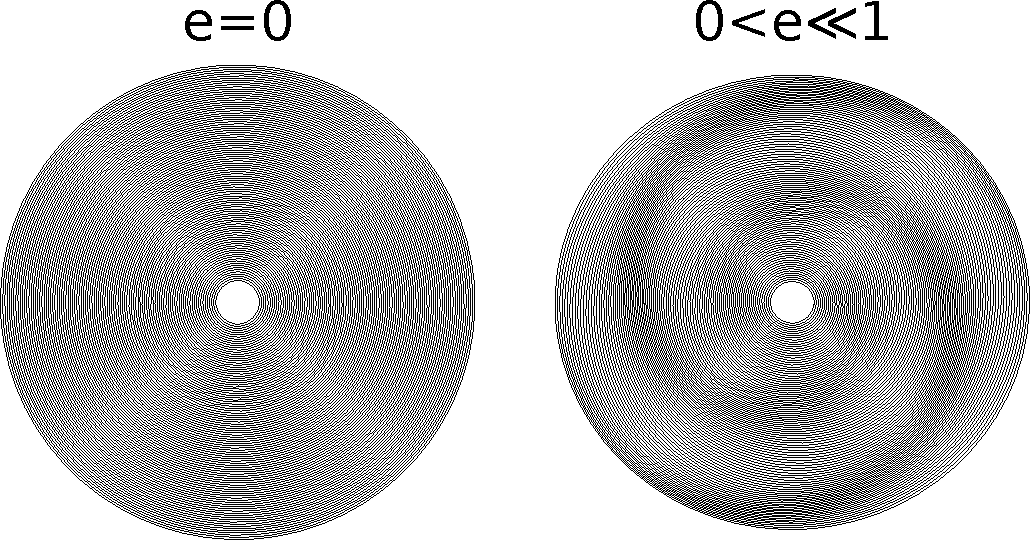
\includegraphics[width=0.9\linewidth]{figure/spiral_arms.pdf}
\caption[Origine des bras spiraux dans une galaxie.]{Illustration de l'origine des bras spiraux dans une galaxie au travers de
l'excitation cohérente de l'excentricité par les bras eux-mêmes. Dans le cas \og $e=0$\fg, les orbites des étoiles, représentées
par les traits noirs sont des cercles parfaits. Dans le cas \og $0<e\ll 1$\fg, les orbites sont toutes très légèrement
excentriques, et les arguments du périhélie légèrement décalés à mesure que les demi-grands axes
augmentent.}\label{fig:spiral_arms}
\end{figure}

\bigskip

Pour l'interaction entre une planète et un disque protoplanétaire, c'est exactement le même principe. Le potentiel de la planète excite les excentricités des éléments fluides voisins jusqu'à former une onde de densité autour de la planète. La différence principale est que le perturbateur est un potentiel gravitationnel tournant, ce qui modifie la forme des ondes de densité comme illustré \reffig{fig:lindblad_torque}. 

\begin{figure}[htbp]
\centering
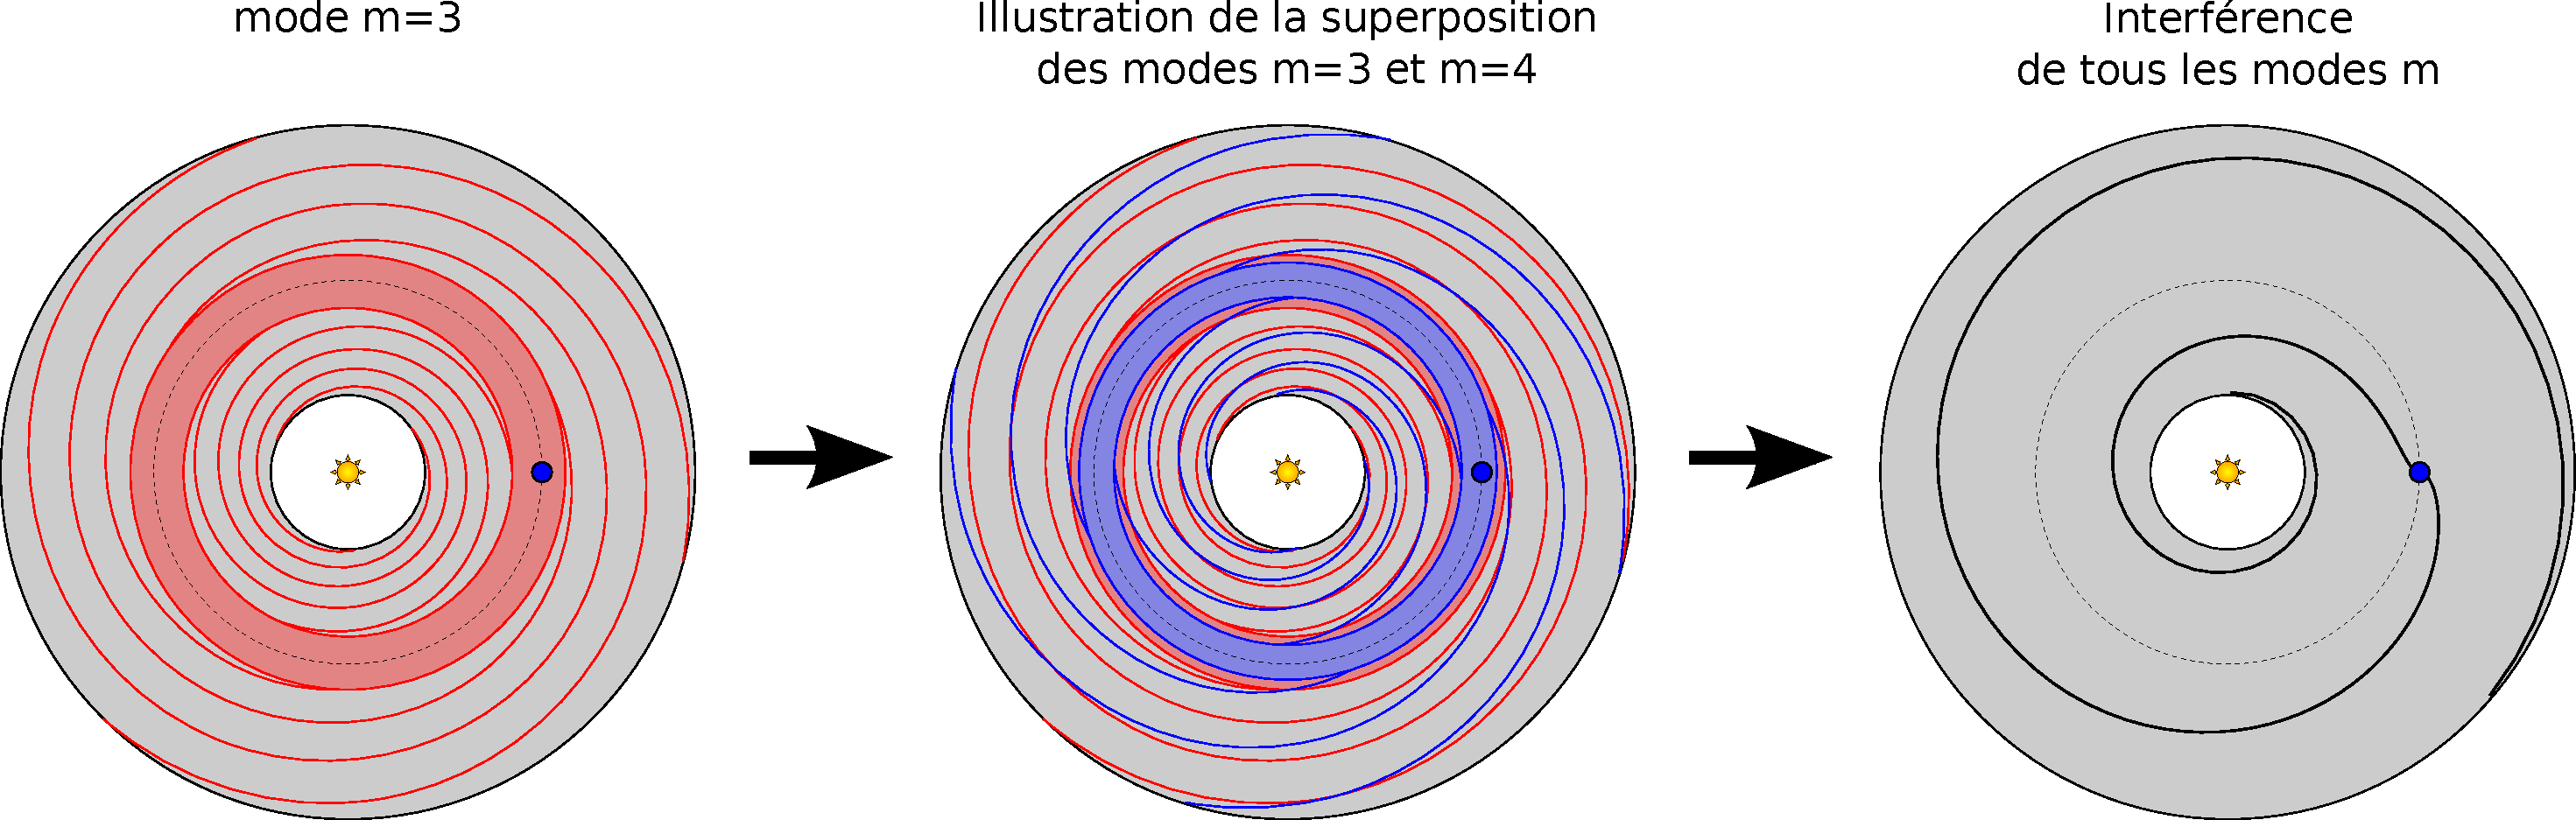
\includegraphics[width=\linewidth]{figure/lindblad_torque.pdf}
\caption[Construction de l'onde de densité due à la présence d'une planète.]{Génération d'ondes de densité dans le disque
protoplanétaire dû à la présence d'une planète. Chaque mode $m$ émet $m$ ondes de densité de part et d'autre de la position
radiale de la planète. Un anneau interne aux positions du mode $m$ est dénué de toute onde dû à ce même mode. Les interférences
entre toutes les ondes de densités de tous les modes donne deux ondes de densités que l'on observe dans des simulations
hydrodynamique. Les positions successives des interférences constructives sont données par \cite[eq. (13) et
(24)]{ogilvie2002wake}}\label{fig:lindblad_torque}
\end{figure}


% discussion avec laurent : L'explication de l'onde de densité avec les excentricités est correct. Ça permet de résoudre le problème du "winding problem", c'est-à-dire que si le bras spiral était rigide, il serait censé s'enrouler sur lui-même au fil de la rotation (vu que la rotation du bras est égale à la rotation des étoiles qui le composent), et donc au bout de quelques rotations, le bras devrait e^tre hyper enroulé. par contre, si on considère une onde de densité, qui n'existe que statistiquement, ça veut dire que les étoiles entre et sortent du bras, qui lui tourne à une vitesse qui lui est propre, et qui n'a rien à voir avec la vitesse des étoiles en elle même. La majorité des galaxies spirales sont barrées, et on pense que c'est la barre quie st à l'origine des spirales, qui démarrent au bout de la barre.

%Par un phénomène résonnant entre une cellule de gaz et un mode $m$ du potentiel gravitationnel de la planète dont on a décomposé l'expression en série de fourrier (on fait ainsi apparaître des termes de fréquence différen

Le potentiel gravitationnel de la planète peut se décomposer en série de Fourier où chaque mode $m$ (entier) a une dépendance sinusoïdale en azimut et possède $m$ maxima et $m$ minima. 

Pour chaque mode $m$ du potentiel gravitationnel de la planète, on définit deux résonances, une résonance interne (ILR : Inner Lindblad Resonance) et une résonance externe (OLR : Outer Lindblad Resonance) associées aux positions suivantes dans le cas d'un disque froid ($H/R\ll 1$ ; \cite{ward1997protoplanet}) : 
\begin{subequations}
\begin{align}
r_{OLR}(m) &= \left(\frac{m+1}{m}\right)^\sfrac{2}{3}r_p\\
r_{ILR}(m) &= \left(\frac{m-1}{m}\right)^\sfrac{2}{3}r_p
\end{align}
\end{subequations}

Pour un mode $m$ donnée, à partir des anneaux de rayon $r_{ILR}(m)$ et $r_{OLR}(m)$ vont être lancées $m$ ondes de densités. 

Dans le cas des bras spiraux dans une galaxie, c'est principalement un mode $m=2$ qui propage une onde spirale de part et d'autre d'une barre centrale source des ondes de densité. Dans le cas d'une planète dans un disque, des ondes de densité sont lancées pour chaque mode $m$. 

Par interférence constructive \citep{ogilvie2002wake}, la somme de toutes les ondes de densités émises par tous les modes du potentiel gravitationnel résulte en la formation d'une onde de densité résultante \reffig{fig:lindblad_torque}. 

\bigskip

Il est important de remarquer que la position de la résonance externe d'ordre $m$ est systématiquement plus proche que la résonance interne associée. Ainsi, en sommant sur tous les modes, on arrive à la conclusion que le couple total externe l'emporte toujours sur le couple total interne \citep{ward1997protoplanet}. 

Ainsi, le couple de Lindblad est généralement négatif pour des modèles typiques de disques protoplanétaires \citep{ward1997protoplanet}.

La résolution numérique des équations linéarisées permet de trouver une formule analytique pour le couple de Lindblad $\Gamma_L$. Dû à la résolution numérique qui doit s'affranchir de la divergence du potentiel gravitationnel en $r=r_0$, cette formule introduit une longueur de lissage permettant de contourner la singularité du noyau du Green du potentiel gravitationnel \citep[eq. (14)]{paardekooper2010torque} : 
\begin{align}
\gamma \Gamma_L/\Gamma_0 &= - \left(2.5 +1.7\beta -0.1d\right) \left(\frac{0.4}{b/h}\right)^{0.71}\label{eq:lindblad-torque}
\end{align}
où $\gamma$ est l'indice adiabatique, $b/h$ le paramètre de lissage du potentiel gravitationnel, et $\beta$ et $d$ sont les exposants des lois de puissance pour les profils de température et de densité de surface. 

Le couple est ici exprimé en unité de $\Gamma_0$, couple de référence défini par : 
\begin{align}
\Gamma_0 &= \left(\frac{q}{h}\right)^2\Sigma_p {r_p}^4 {\Omega_p}^2
\end{align}

Notons aussi que le processus physique du transport du moment cinétique de la planète est réalisé par l'onde de densité. Le moment cinétique est emporté par l'onde de densité qui l'échange avec le gaz environnant à mesure que ce dernier amorti et dissipe l'onde.

\subsubsection{Couple co-orbital ou de corotation}\index{couple!de corotation}\label{sec:couple-corotation}
\begin{figure}[htbp]
\centering
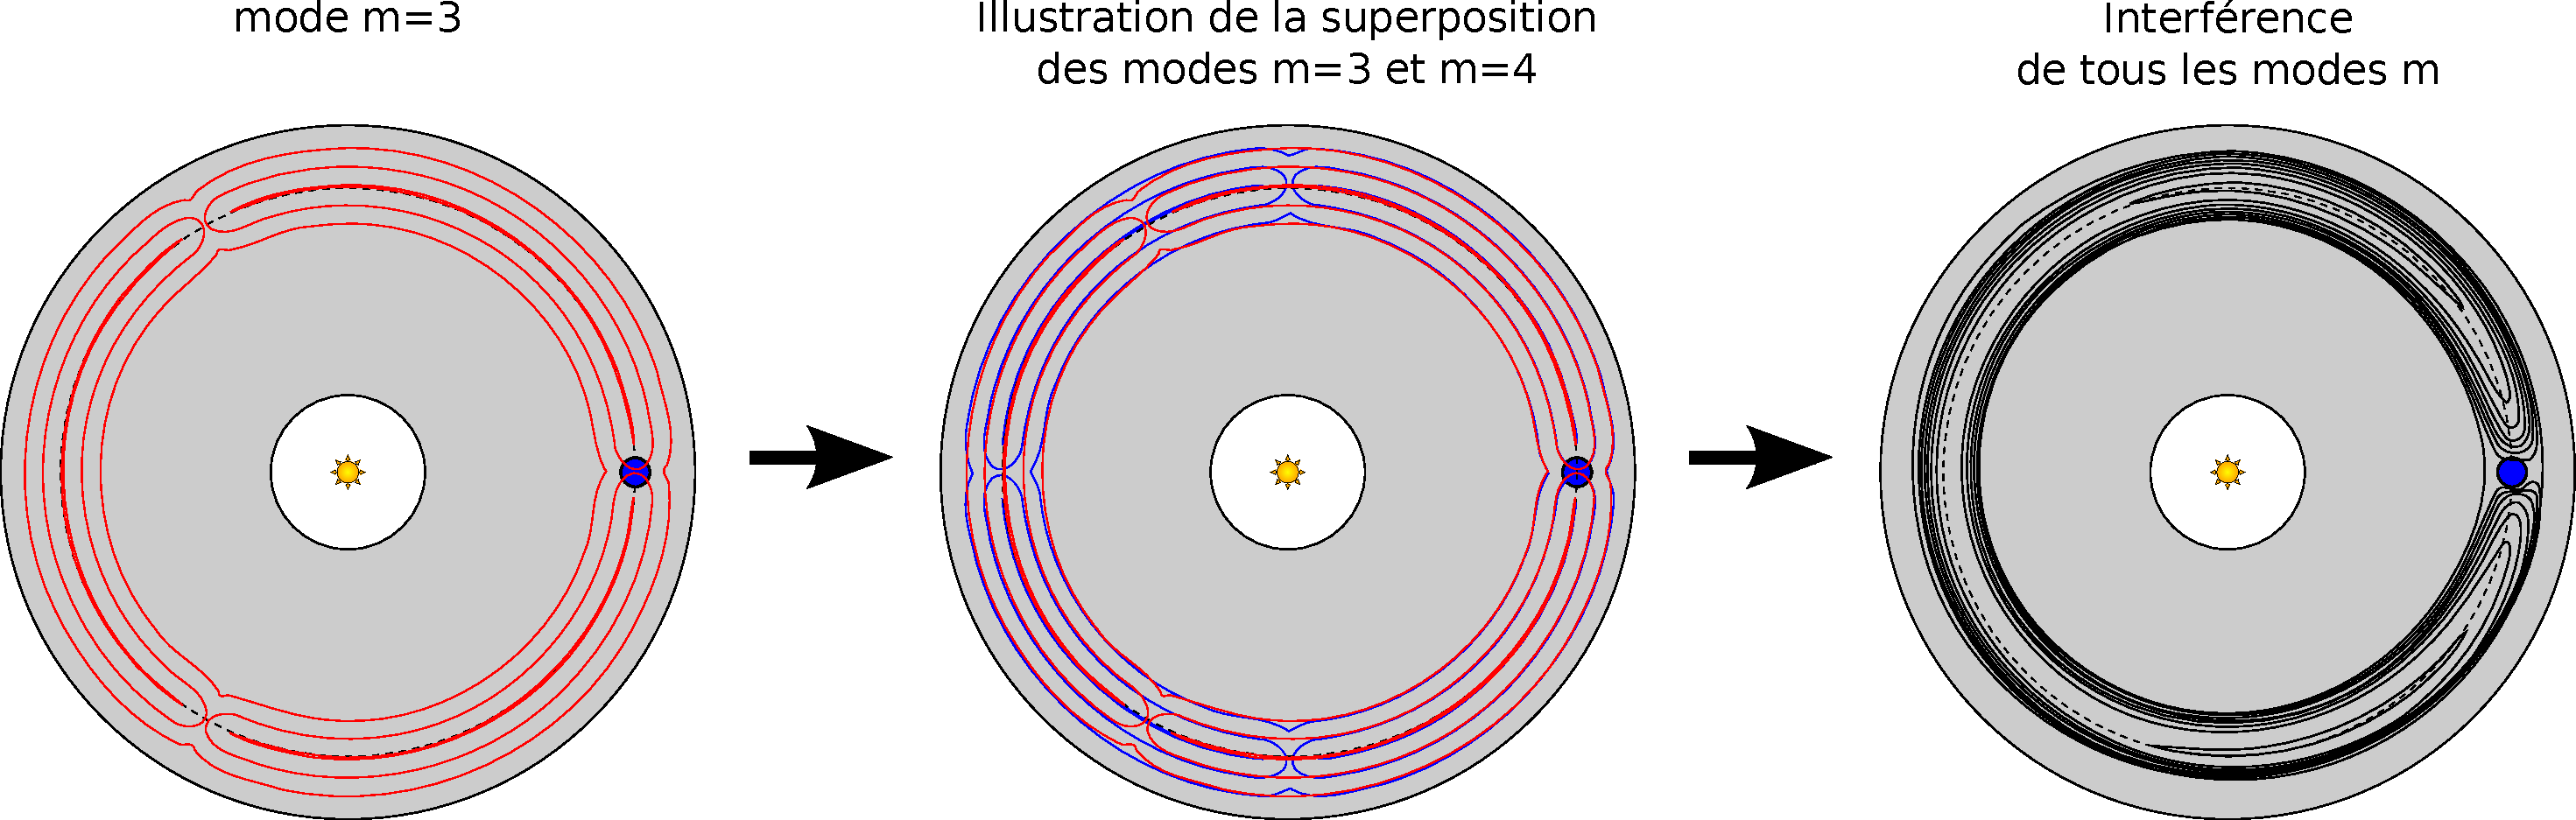
\includegraphics[width=\linewidth]{figure/corotation_modes.pdf}
\caption[Zone de corotation d'une planète.]{À partir de la décomposition en série de Fourier du potentiel
gravitationnel de la planète, chaque mode $m$ a pour conséquence $m$ zones de libration dans la zone de corotation avec la
planète. Les interférences entre l'infinité de modes $m$ fait apparaître des orbites fer-à-cheval (\og horseshoe orbits\fg) dans
le référentiel tournant avec la planète. La zone de corotation a ici été exagérée pour plus de
lisibilité.}\label{fig:corotation_torque}
\end{figure}

De la même manière que précédemment pour le couple de Lindblad, on peut repartir de la décomposition en série de Fourier du potentiel gravitationnel de la planète. Pour chaque mode $m$ de la décomposition, on voit apparaître $m$ zones de libration, centrées sur le rayon de la planète, et réparties en azimut. \reffig*{fig:corotation_torque} représente le mode $m=3$, puis une juxtaposition de mode et finalement le résultat des interférences constructives entre tous les modes $m$ de la décomposition.


Le couple de corotation provient des échanges gravitationnels que va avoir une particule fluide en co-orbite avec une planète. Il existe deux types de couples, issus du gradient de deux quantités physiques distinctes, la vorticité spécifique (vorticité divisée par la densité de surface) appelée parfois vortensité et l'entropie. 

Chacun de ces deux couples possède une partie qui peut saturer en fonction des conditions physiques. 

Pour illustrer le principe de la saturation, et sans considérer un couple en particulier, il convient de définir certains temps caractéristiques afin de comprendre l'origine de ce couple non saturé, et pourquoi ce dernier peut saturer. \reffig*{fig:corotation_orbits} représente schématiquement les 3 temps principaux mis en jeux. 

\begin{figure}[htbp]
\centering
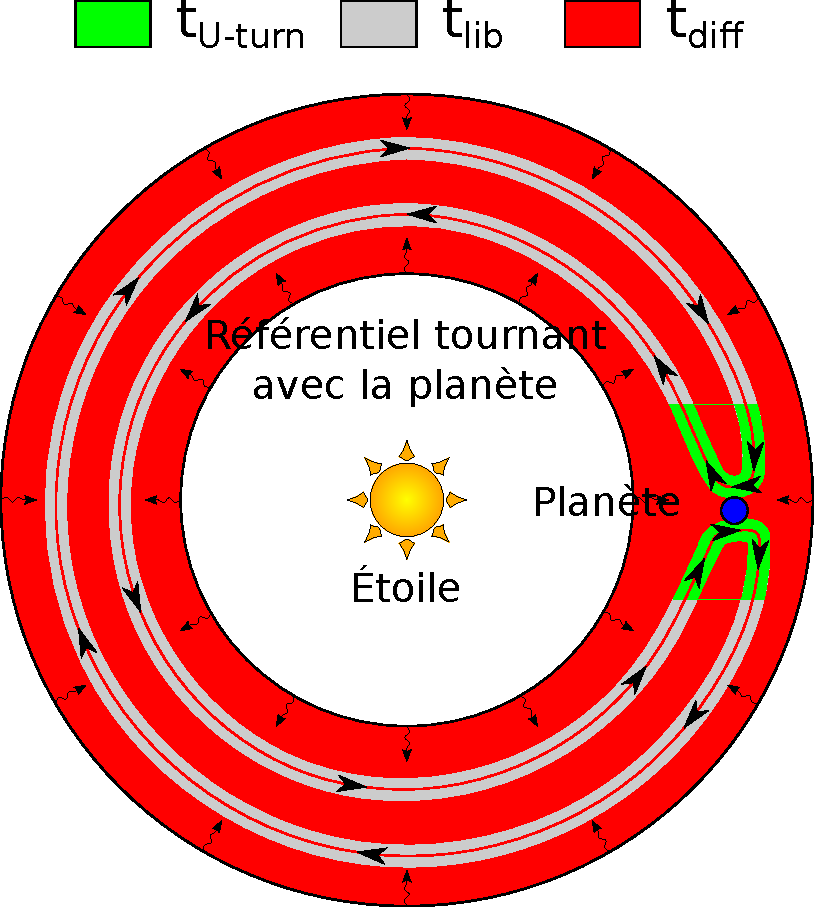
\includegraphics[width=0.75\linewidth]{figure/corotation_times.pdf}
\caption[Temps caractéristiques mis en jeu dans la zone de corotation.]{Dans le référentiel tournant avec la planète (qui est
donc fixe dans ce repère), représentation d'une orbite de corotation ainsi que des différents temps caractéristiques mis en
jeux. $t_\text{lib}$ est le temps mis par un élément fluide pour effectuer une orbite de corotation. $t_\text{U-turn}$ est le
temps mis par un élément fluide pour effectuer un demi-tour devant la planète. $t_\text{diff}$ peut être suivant le cas le temps
radiatif $t_\text{rad}$ ou le temps visqueux $t_\text{vis}$ nécessaire pour homogénéiser les propriétés thermodynamiques de
l'élément fluide avec son environnement.}\label{fig:corotation_orbits}
\end{figure}

On définit tout d'abord $t_\text{lib}$ comme le temps mis par un élément fluide pour effectuer une co-orbite complète dans la zone de fer-à-cheval. Ceci dépend de la distance de l'élément fluide au rayon de corotation. Mais le temps de libration le plus court est obtenu à la distance $x_s$ de la corotation, et vaut \citep[eq. (52)]{baruteau2008corotation} : 
\begin{align}
t_\text{lib} &= \frac{4\pi}{x_s\abs{\od{\Omega}{r}}} = \frac{8\pi r_p}{3\Omega_p x_s}
\end{align}
où $x_s$ est la demi-largeur de la zone de fer-à-cheval (\og half-width of the horseshoe region\fg) \citep[eq. (44)]{paardekooper2010torque} :
\begin{align}
\frac{x_s}{r_p} &= \frac{1.1}{\gamma^{1/4}} \left(\frac{0.4}{b/h}\right)^{1/4} \sqrt{\frac{q}{h}}
\end{align}
Dans le cas d'une planète de $20\unit{M_\oplus}$ à $1\unit{UA}$ dans un disque avec $h=0.05$ et $M_\star=1M_\odot$, ce temps de libration vaut $t_\text{lib}\sim 38 p_\text{orbital}$. 

Le temps $t_\text{U-turn}$ représente quant à lui la durée nécessaire à un élément fluide pour effectuer un demi-tour devant la planète, c'est-à-dire pour parcourir la zone de longueur $2x_s$\footnote{$x_s$ est la demi-largeur de la zone de fer-à-cheval (\og half-width of the horseshoe region\fg)} devant la planète. Il est définit par \citep[eq. (64)]{baruteau2008corotation}
\begin{align}
t_\text{U-turn} &\simeq \frac{4}{\Omega_p}\left[\frac{H(r_p)}{R_H}\right]^\sfrac{3}{2}
\end{align}
où $R_H=r_p (q/3)^{1/3}$ est le rayon de Hill de la planète. Dans le cas d'une planète de $20\unit{M_\oplus}$ à $1\unit{UA}$ dans un disque avec $h=0.05$ et $M_\star=1M_\odot$, ce temps vaut $t_\text{U-turn} \sim 1.6 p_\text{orbital}$.

Un troisième est dernier temps $t_\text{diff}$ rentre en jeu, c'est le temps de diffusion. Selon le processus physique mis en jeu, ce temps peut être $t_\text{rad}$ ou $t_\text{visc}$.

$t_\text{rad}$ représente le temps de diffusion par refroidissement radiatif. Ce temps est plus long quand on se rapproche de l'étoile car le rayonnement est plus rapidement réabsorbé. Le temps radiatif au travers de la zone de corotation est de l'ordre de :
\begin{align}
t_\text{rad} &= \frac{{x_s}^2}{\chi}
\end{align}
où $x_s$ est la demi-largeur de la zone de corotation et $\chi$ est la diffusivité thermique.
 
$t_\text{visc}$ représente la diffusion d'une quantité physique par la viscosité. Ce temps est plus court quand on se rapproche de l'étoile. Le temps visqueux à la zone de corotation $t_\text{visc}$ est  de l'ordre de \citep{masset2001coorbital, masset2002coorbital, ogilvie2003saturation}
\begin{align}
\tau_\nu &\sim \frac{{x_s}^2}{\nu}
\end{align}

Quand la grandeur physique considérée est la vortensité (ou vorticité spécifique), seul $t_\text{visc}$ est à prendre en compte. Quand c'est l'entropie, les deux temps $t_\text{visc}$ et $t_\text{rad}$ sont importants. \reffig*{fig:corotation_orbits} récapitule les temps mis en jeux et à quoi ils correspondent.

\bigskip

Pour que le couple de corotation soit non saturé, on doit satisfaire aux inéquations suivantes \citep[eq. (31)]{baruteau2013recent} :
\begin{align}
t_\text{U-turn} < t_\text{diff} < \frac{t_\text{lib}}{2}
\end{align}
$t_\text{U-turn}$ est le temps nécessaire pour faire le demi-tour devant la planète (pour traverser une zone égale approximativement à $2x_s$). $t_\text{lib}$ est le temps de libration, c'est-à-dire le temps mis par une particule fluide pour faire le tour de la zone en fer-à-cheval. $t_\text{diff}$ quant à lui est le temps de diffusion de la quantité physique considérée. Suivant les cas, il peut y avoir plusieurs temps de diffusion qui sont importants, auquel cas les inégalités doivent être satisfaites pour tous les temps de diffusions mis en jeux.

\begin{figure}[htbp]
\centering
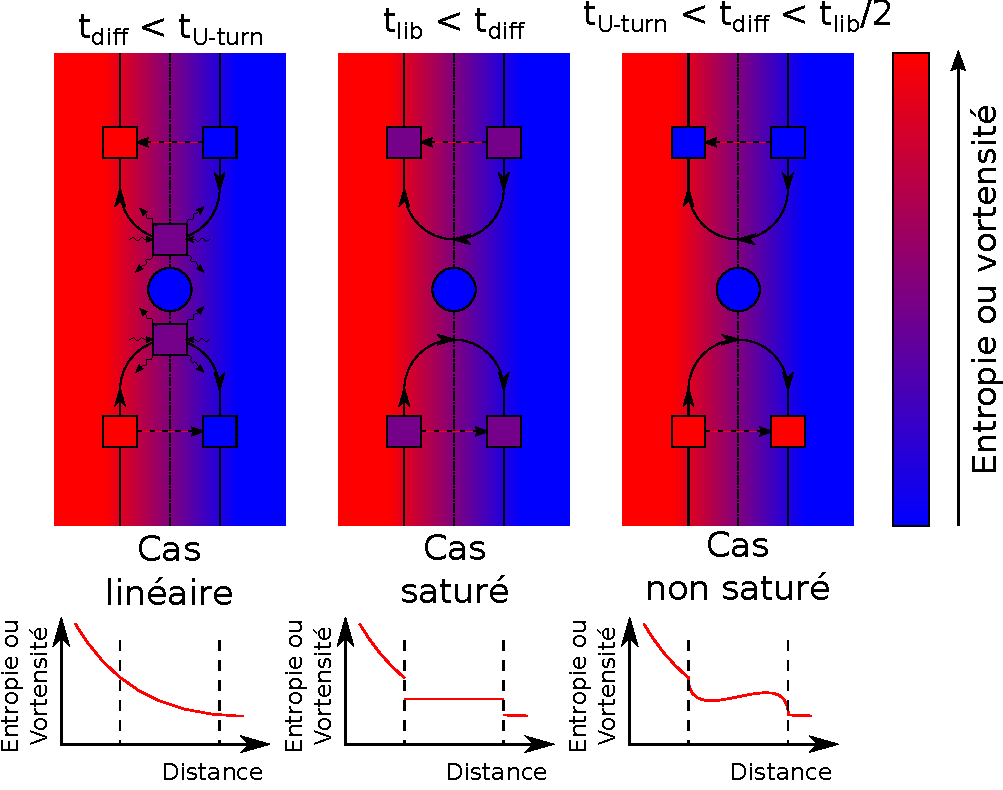
\includegraphics[width=0.75\linewidth]{figure/corotation_principle.pdf}
\caption[État du couple de corotation en fonction des valeurs des temps caractéristiques.]{Dans le référentiel tournant avec la
planète, représentation du mécanisme général à l'origine du couple de corotation. Lorsque les temps de diffusion $t_\text{diff}$
sont plus grands que le temps de libration $t_\text{lib}$, le couple de corotation sature car le gradient de vortensité/entropie
au travers de la région fer-à-cheval tend à s'aplatir. Ce dernier est restauré quand les temps de diffusion $t_\text{diff}$ sont
plus courts que le temps de libration $t_\text{lib}$. Dans ce cas, la valeur optimale du couple de corotation est obtenue
lorsque les temps de diffusion $t_\text{diff}$ sont de l'ordre de la moitié du temps de libration $t_\text{lib}/2$. Dans la
limite où les temps de diffusion $t_\text{diff}$ sont plus courts que le temps de demi-tour $t_\text{U-turn}$, l'amplitude du
couple de corotation décroit pour atteindre la valeur prédite par une analyse linéaire.}\label{fig:corotation_principle}
\end{figure}

\reffig*{fig:corotation_principle} illustre les trois cas possibles en fonction des commensurabilités entre les différents temps caractéristiques mis en jeux.

L'idée générale afin d'éviter la saturation, c'est qu'on doit restaurer le gradient d'entropie / de vortensité au travers de la zone fer-à-cheval. Il faut donc que les processus diffusifs soient suffisamment efficace pour qu'en arrivant à la région de \og U-turn\fg de l'autre côté, l'élément fluide ait pu équilibrer ses conditions physiques avec le milieu environnant. Cette condition est illustrée par l'inégalité suivante : 
\begin{align}
t_\text{diff} < \frac{t_\text{lib}}{2}
\end{align}

Mais il faut de plus que la diffusion ne soit pas trop efficace, sous peine que la valeur du couple de corotation diminue pour atteindre la valeur prédite par une analyse linéaire. Ceci donne alors la deuxième inéquation : 
\begin{align}
t_\text{U-turn} < t_\text{diff}
\end{align}

\bigskip

De la même manière que pour le couple de Lindblad, la résolution numérique des équations nous permet d'avoir des expressions analytiques pour les couples de corotation. 

Il y a d'une part les couples soumis à saturation \citep[eq. (45)]{paardekooper2010torque} :
\begin{subequations}
\begin{align}
\gamma \Gamma_\text{c,hs,baro}/\Gamma_0 &= 1.1\left( \frac{3}{2} - d\right)\left(\frac{0.4}{b/h}\right)\\
\gamma \Gamma_\text{c,hs,ent}/\Gamma_0 &= \frac{\xi}{\gamma}\left(10.1\sqrt{\frac{0.4}{b/h}} - 2.2\right)\left(\frac{0.4}{b/h}\right)
\end{align}\label{eq:saturated-corotation-torque}
\end{subequations}
et les couples non soumis à saturation, dits linéaires \citep[eq. (17)]{paardekooper2010torque} :
\begin{subequations}
\begin{align}
\gamma \Gamma_\text{c,lin,baro}/\Gamma_0 &= 0.7\left( \frac{3}{2} - d\right)\left(\frac{0.4}{b/h}\right)^{1.26}\\
\gamma \Gamma_\text{c,lin,ent}/\Gamma_0 &= \xi\left[2.2\left(\frac{0.4}{b/h}\right)^{0.71} - \frac{1.4}{\gamma}\left(\frac{0.4}{b/h}\right)^{1.26}\right]
\end{align}\label{eq:linear-corotation-torque}
\end{subequations}
$d$ et $\xi=\beta - (\gamma-1)d$ sont respectivement les négatifs des exposants des lois de puissance pour les profils 1D de densité de surface et d'entropie.

\bigskip

Dans la pratique, ce couple peut être positif (migration vers l'extérieur) ou négatif (migration vers l'intérieur) en fonction des variations des quantités physiques par rapport à leur valeur nominales.

\subsubsection{Modélisation dans le code N-corps}
Les couples de Lindblad et de Corotation ont été intégrés aux simulations numériques en utilisant le modèle de \cite{paardekooper2011torque}. Plus de détails sur l'implémentation de ces formules et le modèle de disque utilisé dans la section \refsec{sec:code_n-corps}.

\subsection{Migration des planètes massives : Type II}\index{migration!Type II}
Par massive, on entend une planète qui va induire des modifications importantes du profil de densité du disque. L'approximation du régime linéaire n'est alors plus valable. 

Je présente ici très succinctement ce type de migration que je n'ai pas considéré tout au long de ma thèse. Je me place dans le régime linéaire et me suis concentré sur les cœurs de planète géante et les planètes telluriques. J'ai donc négligé tous les effets non-linéaires dû aux grandes masses, et en particulier la création d'un sillon par les planètes.

\bigskip

Quand une planète dans un disque devient suffisamment massive, la réponse du disque n'est plus linéaire, et des ondes de densité induites par la planète forment des chocs non loin de là où elles sont émises. La répulsion entre le disque et la planète devient si forte qu'une cavité annulaire se forme autour de l'orbite de la planète, creusant le disque de gaz \citep{lin1986tidal}.

Une fois que la cavité est formée, la planète est dite en migration de \gras[migration!Type II]{Type II} : son orbite agit alors essentiellement comme une barrière entre les deux parties du disque de gaz, \emph{interne} et \emph{externe}. Du gaz peut sauter le gap \citep{lubow2006gas}, ou être accrété par la planète mais cette dernière voit son mouvement régit par le disque de gaz, se retrouvant entraînée par la migration de celui-ci.

Quand la planète creuse un sillon et que sa masse est inférieure ou de l'ordre de la masse locale du disque ($M_p \lesssim M_\text{d,loc}$ avec lequel elle interagit, alors le temps de migration de la planète est contrôlé par le temps visqueux du disque, car cette dernière se comporte comme une particule de ce disque \citep{nelson2000migration}.

\bigskip

Pendant que le gap dû à la planète est en train de se creuser, il peut y avoir un fort couple de corotation négatif \citep{masset2003runaway}. Ce mode de migration intermédiaire est parfois appelé migration de \gras[migration!Type III]{Type III}. 

\subsection{L'amortissement de l'excentricité et de l'inclinaison}\index{amortissement!excentricité}\index{amortissement!inclinaison}%circularisation
%Penser aux papiers cresswell et al. 2007 et tanaka et al. 2004
Une planète sur une orbite non-circulaire $e\neq 0$ génère des ondes supplémentaires à cause de son excentricité. De même, une orbite légèrement inclinée induit des ondes à cause de l'inclinaison $I$ de la planète. 

Des calculs analytiques sur les équations linéarisées (valables quand $e$ et $I$ sont faibles $e,i \ll H/R$) montrent que les ondes dues à l'excentricité ou l'inclinaison ont tendance à amortir l'élément orbital qui est à leur origine. \cite[eqs. (45), (47)]{tanaka2004three} trouvent un amortissement exponentiel dont les temps caractéristiques sont : 
\begin{subequations}
\begin{align}
\frac{\overline{\dot{e}}}{e} &= -\frac{0.780}{t_\text{wave}}\\
\frac{\overline{\dot{I}}}{I} &= -\frac{0.544}{t_\text{wave}}
\end{align}
\end{subequations}
où le temps caractéristique de l'évolution orbitale $t_\text{wave}$ est donné par \cite[eq. (49)]{tanaka2004three} :
\begin{align}
t_\text{wave} &= \frac{M_\star}{M_p}\frac{M_\star}{\Sigma_p a^2} \left(\frac{H}{R}\right)^4 {\Omega_p}^{-1}
\end{align}

Le temps caractéristique d'amortissement pour l'excentricité et l'inclinaison est similaire et de l'ordre de \citep{tanaka2004three} :
\begin{align}
\tau_e \sim \tau_I &\sim h^2 \tau_\text{mig}
\end{align}

Des simulations hydrodynamiques montrent que le même phénomène d'amortissement se produit pour des valeurs plus grandes de $e$ et $I$, tout en étant dans un régime différent que celui à faibles valeurs ($e,i \ll H/R$) \citep{cresswell2007evolution}. On explique cela pour l'inclinaison par le fait qu'à grande inclinaison, la planète peut sortir du disque est ressentir un amortissement réduit. Pour l'excentricité quant à elle, on invoque le fait que durant son orbite la planète va voir sa vitesse varier par rapport à celle du disque de gaz \citep{papaloizou2000orbital}.

\subsection{L'accrétion du gaz}\label{sec:accretion_coeur}\index{accrétion de gaz}
Dans le modèle d'accrétion de cœur, les planètes géantes sont d'abord des cœurs rocheux qui grossissent jusqu'à atteindre une masse critique de l'ordre de $10 M_{\oplus}$ \citep{pollack1996formation}. Une fois cette masse atteinte, le cœur commence à accréter rapidement du gaz jusqu'à former une géante gazeuse.

Ceci implique que la formation des planètes géantes doive se passer avant que le disque de gaz ne se dissipe (ce qui intervient au bout de quelques millions d'années).

Les noyaux de ces planètes sont supposés se former au-delà de la ligne des glaces (limite radiale virtuelle au delà de laquelle on peut trouver de l'eau sous forme solide ; autour de $4\unit{UA}$ \citep{martin2013evolution}). En effet, au delà de cette limite, la quantité de matière solide augmente, et donc le taux d'accrétion augmente aussi \citep{sasselov2000snowline}.

La formation des embryons de planètes géantes n'est toujours pas claire. On ne sait pas vraiment s'il y a une zone privilégiée ou non, la limite virtuelle de la ligne des glaces pourrait ne pas être valable, la glace ne rajoutant qu'environ 50\% de masse en plus \citep{lodders2003solar}.\index{ligne des glaces}


\bigskip

Pour une simulation donnée, si on augmente le taux d'accrétion de la planète, celle-ci sera plus massive, et aura donc une inertie plus grande. Elle mettra donc plus de temps à migrer\index{migration} par migration de Type II car son inertie s'y opposera. D'un autre côté, si la planète n'a pas encore créé de gap, la migration de Type I est plus rapide à mesure que la masse augmente. 

\subsection{Récapitulatif des interactions dans le code N-corps}
Numériquement, le couple de la migration de Type I est pris en compte en utilisant les formules semi-analytiques développées par \cite{paardekooper2011torque}. 

L'amortissement de l'inclinaison et de l'excentricité quant à elles sont modélisées via les formules de \cite{cresswell2008three}.



\chapter{Le Code N-Corps}
Afin d'étudier la formation planétaire et les interactions avec le disque de gaz, j'ai utilisé un code de simulation N-corps, qui permet de regarder l'évolution d'un nombre arbitraire de corps orbitant autour d'un astre central \citep{chambers1999hybrid}. 

Ce choix est apparu naturellement. Au début de ma thèse, j'ai fait quelques simulations hydrodynamiques avec le code Genesis développé par Arnaud Pierens. J'ai rapidement constaté que ce genre de simulations, bien que modélisant de manière poussée le disque, ne permettait pas d'étudier de manière approfondie la dynamique planétaire. Le temps de calcul nécessaire pour une simulation limite en effet grandement le nombre de corps ainsi que la durée d'intégration. J'ai donc souhaité me tourner vers un code N-corps, afin de privilégier la dynamique planétaire, et de modifier ce programme afin d'y inclure les effets d'un disque de gaz sur la dynamique planétaire. 

J'ai ainsi gagné en temps de calcul, et j'ai ouvert un vaste champ d'investigation sur les paramètres du disque, le nombre de corps en interaction, me permettant de faire des systèmes planétaires très divers, parfois avoir plusieurs centaines d'embryons pour plusieurs millions d'années, chose impossible dans les simulations hydrodynamiques du début de ma thèse où 20 corps pendant quelques dizaines de milliers d'années était un maximum. 

Ce choix a bien entendu introduit son lot d'incertitudes et d'approximations qui sont discutées dans la partie \refsec{sec:discussion}. La présente partie a pour but de présenter le code N-corps que j'ai développé ainsi que les différents effets du disque que j'ai modélisé. J'ai avant tout souhaité présenter les parties qui ont des conséquences sur la physique du disque, que ce soit en terme de choix d'un modèle particulier, ou de limitations numériques qu'il est bien de garder à l'esprit quand on interprète les résultats.

\section{Présentation de Mercury}\index{logiciel!Mercury}
Le code N-corps choisi est le code \textbf{Mercury} \citep{chambers1999hybrid}. Ce code offre la possibilité de choisir un algorithme parmi 5 différents (BS, BS2, RADAU, MVS et HYBRID), ayant des propriétés diverses. Dans le cadre de ma thèse, je n'ai utilisé que l'algorithme HYBRID, qui utilise l'algorithme MVS la plupart du temps, mais change pour l'algorithme BS2 lors de rencontres proches. 

La raison de ce changement est assez simple. MVS est un algorithme symplectique \citep{wisdom1991symplectic}, c'est-à-dire à pas de temps constant, dans lequel on définit un hamiltonien que l'on résout pour faire évoluer les orbites. La conservation de l'énergie est moins bonne que pour un algorithme à pas de temps adaptatif, mais le point très important est que cette conservation de l'énergie est bien meilleure au cours du temps. c'est-à-dire que là où les algorithmes tels que BS, BS2 et RADAU verront leur erreur sur l'énergie augmenter au cours du temps, les algorithmes symplectiques vont eux voir leur erreur rester plus ou moins constante au cours du temps. 

Dans le cadre de mes simulations, j'ai accordé une importance limitée aux variations d'énergie, étant donné que les couples que l'on rajoute pour simuler la présence du disque de gaz font que l'énergie n'est pas conservée pour une planète donnée. Cependant, il est important de bien résoudre les orbites et c'est ce point qui est le plus crucial ici. En effet, quelques tests ont permis de contraindre le pas de temps minimal qu'il est nécessaire d'avoir en fonction de la distance orbitale d'une planète. La contrainte de pas de temps dans mes simulations vient donc d'une distance minimale en dessous de laquelle les orbites ne sont pas correctement calculées. Cette limite, afin d'éviter tout problème, est choisie pour être en dessous du bord interne du disque de gaz que je définis.

Les détails techniques et les options de mon code sont détaillés dans l'annexe \refsec{sec:nbody-readme}.

\section{Algorithmes d'intégration}
Dans Mercury, il y a cinq algorithmes différents à notre disposition :
\begin{itemize}
\item MVS \citep{wisdom1991symplectic} : un code symplectique\footnote{Basiquement, un code symplectique est un code qui conserve parfaitement l'énergie de par sa définition en terme d'hamiltoniens.}, c'est-à-dire qui conserve l'énergie au cours du temps et dont le pas de temps est fixe (c'est le seul à avoir un pas de temps fixe)
\item BS \citep{stoer1980introduction} : un algorithme à pas de temps variable, réputé robuste et plutôt long à tourner.
\item BS2 \citep{press1992numerical} : Basé sur BS, il présente l'inconvénient de ne pas fonctionner pour les systèmes non conservatifs. Il est censé être deux fois plus rapide que BS.
\item RADAU \citep{everhart1985efficient} : Ne fonctionne pas bien pour les rencontres proches et les orbites très excentriques. Est censé être deux à trois fois plus rapide que BS.
\item HYBRID \citep{chambers1999hybrid} : Ce code utilise MVS en temps normal, puis lors d'une rencontre proche, utilise BS2 afin de résoudre correctement les orbites.
\end{itemize}

Il y a donc principalement deux catégories : les intégrateurs symplectiques où le paramètre fixe est le pas de temps ($h=\cte$) et les intégrateurs N-corps où le paramètre est la précision en terme de conservation d'énergie d'un pas de temps à l'autre (le pas de temps n'étant pas fixe). Ici, seuls MVS et HYBRID utilisent une partie symplectique alors que BS, BS2 et RADAU sont purement N-corps.

\bigskip

On définit le Hamiltonien $H$ de notre problème N-corps comme étant la somme des énergies cinétiques et potentielles de chaque corps : 
\begin{align}
H &= \sum_{i=1}^N\frac{{p_i}^2}{2m_i} -G\sum_{i=1}^N\sum_{j=i+1}^N\frac{m_im_j}{r_{ij}}
\end{align}
où $m_i$ est la masse du corps $i$, $p_i$ son impulsion et $r_{ij}$ la séparation entre les corps $i$ et $j$.

Un intégrateur symplectique est un intégrateur qui au lieu d'appliquer directement le hamiltonien $H$ sur le système, va séparer ce dernier en deux (ou plusieurs parties) et appliquer ces sous-hamiltoniens successivement. Un intégrateur symplectique résout donc le problème de manière approchée en négligeant les termes croisés des sous-hamiltoniens.

Afin de minimiser l'erreur due à cette approximation, il faut choisir judicieusement la séparation du hamiltonien afin d'avoir une partie dominante par rapport à l'autre.

Par définition, un algorithme symplectique conserve l'énergie au cours du temps, même si l'énergie fluctue au cours du temps autour d'une valeur moyenne. 

Les intégrateurs symplectiques ont deux avantages importants sur les intégrateurs classiques : 
\begin{enumerate}
\item Les fluctuations \og instantanées\fg de l'énergie dues à un algorithme symplectique sont plus grandes que celles d'un
algorithme N-corps, mais à la différence de ces derniers, l'erreur ne croit pas au cours du temps \reffig{fig:energy_error}.
\item Ils sont moins couteux en temps de calcul, en particulier quand la majeure partie de la masse est contenue dans un seul corps (bien adapté pour l'étude d'un système planétaire autour d'une étoile donc).
\end{enumerate}

\begin{figure}[htbp]
\centering
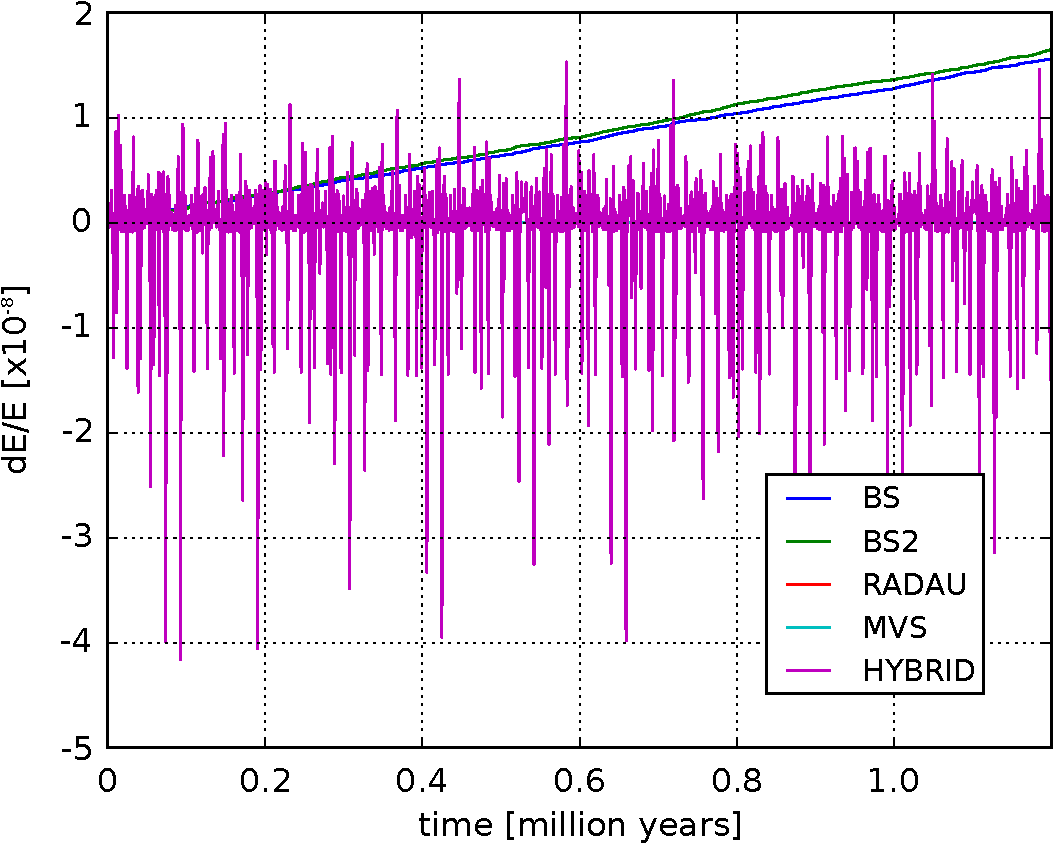
\includegraphics[width=0.65\linewidth]{figure/energy_error.pdf}
\caption[Pour une même simulation, erreur au cours du temps pour BS, BS2, RADAU, MVS et HYBRID.]{Évolution de l'erreur au cours
du temps pour une simulation contenant trois planètes d'une masse terrestre chacune, cette simulation étant lancée
successivement avec chacun des algorithmes disponibles dans \textbf{Mercury}. Les lignes correspondant 
aux intégrateurs MVS et RADAU sont superposées et confondues avec la ligne $\dif E/E=0$.}\label{fig:energy_error}
\end{figure}

Les algorithmes symplectiques ont cependant un inconvénient. Le pas de temps fixe d'un intégrateur symplectique ne permet pas de résoudre correctement les rencontres proches entre les corps du système. Chaque fois que le pas de temps d'un algorithme symplectique est changé, son hamiltonien change aussi, et entraine une variation d'énergie du système (dont l'énergie va osciller autour d'une nouvelle valeur moyenne). 

\bigskip

Nous cherchons maintenant à déterminer l'algorithme le plus approprié pour notre étude. Nous souhaitons faire évoluer un système avec plusieurs dizaines d'embryons planétaires pour plusieurs millions d'années, le système n'étant pas conservatif à cause des divers effets du disque que nous implémentons. 

Nous souhaitons résoudre correctement les orbites, mais avoir un temps de calcul raisonnable. 

La première contrainte est la dissipation. En effet, notre système n'est pas conservatif. Tous les algorithmes N-corps disponibles (BS, BS2 et RADAU) ne fonctionnent donc pas correctement, ces derniers réclament un pas de temps extrêmement faible qui n'est pas représentatif de la précision demandée pour l'intégration N-corps, la variation d'énergie numérique étant masquée par la variation d'énergie induite par les effets du disque. 

Il nous reste les algorithmes MVS et HYBRID. La deuxième contrainte, ce sont les rencontres proches et les collisions. Nous savons qu'un algorithme symplectique ne les traite pas correctement, et si c'est une erreur négligeable dans le cas où il y en a peu, ça ne l'est absolument plus dans notre cas, le nombre de rencontres proches pouvant être très important, notamment dans la phrase d'accrétion en début de simulation. L'algorithme MVS ne parait donc pas adapté contrairement à HYBRID qui a été construit pour être à la fois symplectique et gérer correctement les rencontres proches moyennant une erreur plus importante lors du changement d'algorithme. 

L'algorithme HYBRID est l'algorithme MVS, à pas de temps constant la majorité du temps. Il a donc les avantages d'un algorithme symplectique, à savoir la conservation de l'énergie et la rapidité d'exécution. Lors de rencontres proches (déterminées par une distance minimale d'approche entre deux corps, soit en rayon de Hill, soit en nombre de pas de temps), l'algorithme BS2 est utilisé, le pas de temps devient donc variable afin de résoudre correctement la rencontre et éventuellement la collision. Une fois fini, c'est de nouveau MVS qui prend le relai \citep[voir aussi ][]{mcneil2009new}. 

Dans notre cas, plusieurs approximations sont faites : 
\begin{itemize}
\item L'algorithme BS2 ne fonctionne que pour les systèmes conservatifs. On suppose que la variation d'énergie induite par la migration est totalement négligeable pendant le bref laps de temps de la rencontre proche
\item Le nombre de rencontres proches est suffisamment faible pour que les propriétés symplectiques de l'intégrateur soient 
conservées. On suppose de plus que les variations d'énergies induites par ce biais sont négligeables devant la dissipation 
induite par le disque (qui est de l'ordre de l'énergie initiale du système planétaire)
\end{itemize}

Il reste alors une chose à déterminer, c'est le pas de temps fixe que l'on doit choisir afin de résoudre correctement les orbites. Pour cela, on se place dans un cas simplifié, sans les effets du disque, et on souhaite savoir la condition sur le pas de temps afin que l'orbite soit correctement calculée. 

On ne s'intéresse qu'aux orbites internes qui sont limitantes au niveau du pas de temps en raison de leur période réduite. Pour une planète à une distance de $0.1\unit{UA}$ du soleil, la période orbitale est de 11 jours environ.

On réalise deux tests. Dans le premier test, on fait évoluer une planète de $1\mearth$ totalement isolée. On fait varier son demi-grand axe et son excentricité et on regarde comment évolue la conservation de l'énergie. Étant donné qu'avec un algorithme symplectique l'énergie oscille au cours du temps, on prend la valeur moyenne de la variation d'énergie, moyenne effectuée sur une centaine de valeurs.

Dans un deuxième test, on procède exactement de la même manière, à ceci près qu'on place une planète de $1\unit{M_\text{jup}}$ à $5\unit{UA}$. 

\reffig{fig:accuracy_maps} montre l'évolution de la conservation de l'énergie dans ces deux tests pour deux pas de temps différents, $h=1\unit{jour}$ et $h=0.4\unit{jour}$. Pour un pas de temps donné, nous ne pouvons pas donner simplement de position en dessous de laquelle l'orbite n'est pas correctement résolue. L'excentricité a une influence. En effet, la distance minimale entre l'étoile et la planète se situe au périhélie, mais suivant l'excentricité, la planète passera plus ou moins de temps au périastre. Ainsi, une très grande excentricité va diminuer drastiquement le temps passé au périastre, pour un périastre donné \citep{rauch1999dynamical, levison2000symplectically}. 

\begin{figure}[htbp]
\centering
\subfloat[$h=1\unit{jour}$ sans Jupiter]{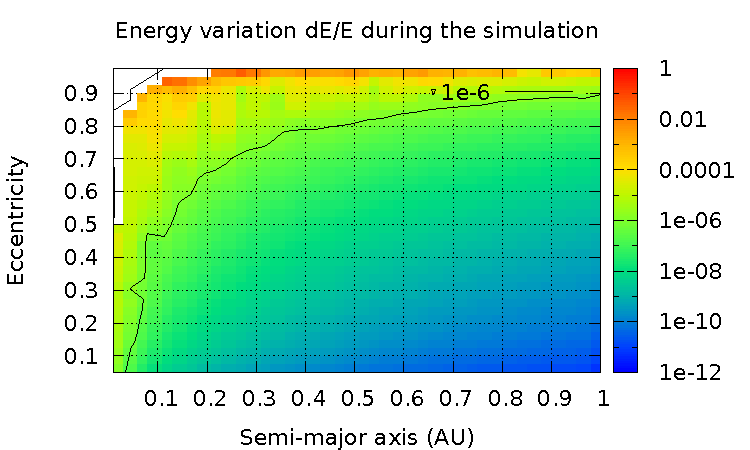
\includegraphics[width=0.49\textwidth]{figure/accuracy_10_one.pdf}}\hfill
\subfloat[$h=1\unit{jour}$ avec Jupiter]{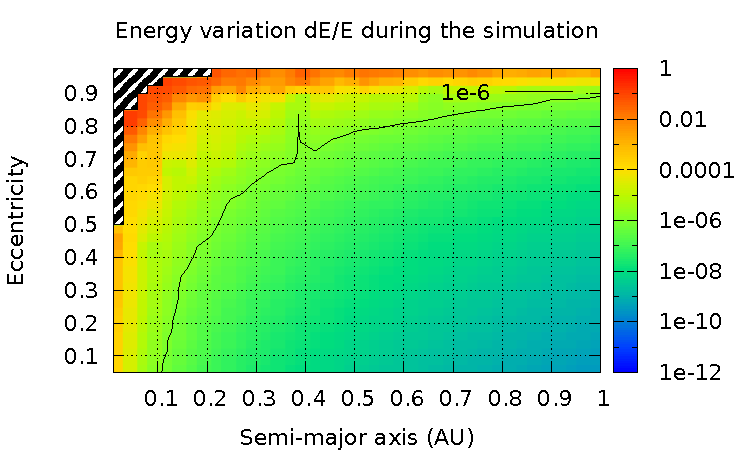
\includegraphics[width=0.49\textwidth]{%
figure/accuracy_10_jup.pdf}}

\subfloat[$h=0.4\unit{jour}$ sans Jupiter]{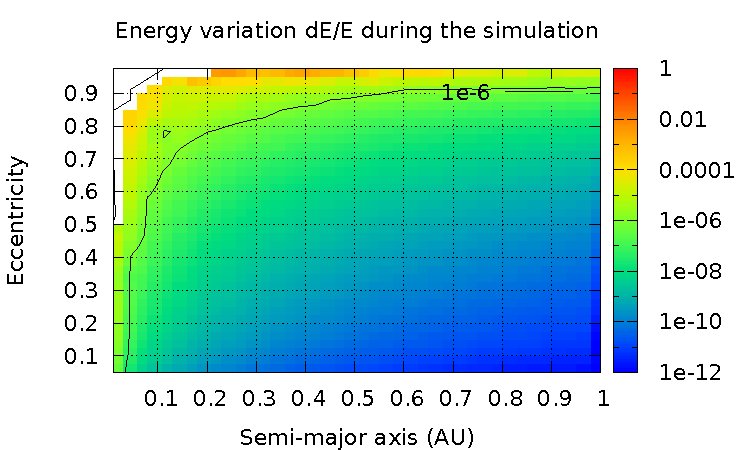
\includegraphics[width=0.49\textwidth]{figure/accuracy_04_one.pdf}}\hfill
\subfloat[$h=0.4\unit{jour}$ avec Jupiter]{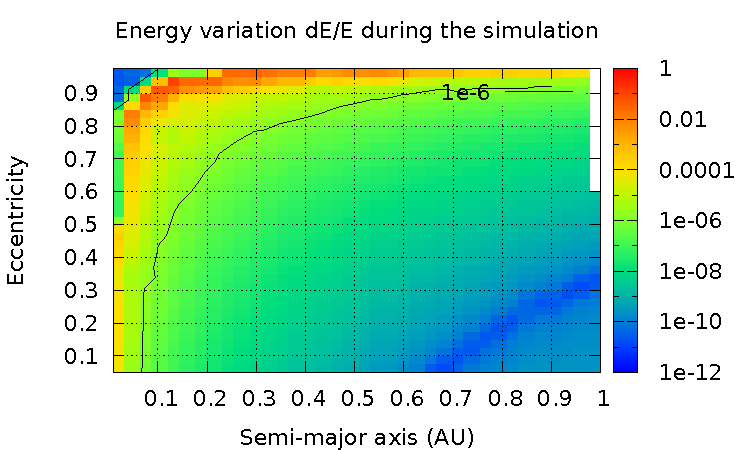
\includegraphics[width=0.49\textwidth]{%
figure/accuracy_04_jup.pdf}}


\caption[Conservation de l'énergie en fonction du pas de temps et des conditions initiales.]{Tests pour $h=1\unit{jour}$ et
$h=0.4\unit{jour}$ de la conservation de l'énergie pour une planète de $1\mearth$ isolée ou avec un compagnon de la taille de
Jupiter. Les cartes montrent la conservation de l'énergie pour différentes valeurs du demi-grand axe $a$ et de l'excentricité
$e$. La ligne noire correspond à un $\dif E/E=10^{-6}$, valeur en dessous de laquelle on considère que la précision sur l'orbite
est suffisante. La partie hachurée correspond à la collision de la planète interne avec l'étoile centrale donc le rayon est
$R_\star=0.005\unit{UA}$.}\label{fig:accuracy_maps}
\end{figure}

Si un pas de temps plus grand ($h=1\unit{jour}$) semble convenir pour une planète isolée, la conservation de l'énergie est
différente dans le cas avec des perturbations gravitationnelles (cas avec Jupiter). À $0.1\unit{UA}$, qui correspond au bord
interne, zone particulièrement importante pour notre étude, ce pas de temps ne convient plus. Dès que l'excentricité augmente un
peu, la précision sur l'orbite diminue, et les orbites les plus internes ne sont pas correctement résolues.

Même si le disque amortit les excentricités, nous souhaitons résoudre correctement les orbites légèrement excentriques, même au bord interne à $0.1\unit{UA}$. Un pas de temps de $h=1\unit{jour}$ résout correctement les orbites au bord interne, même légèrement excentriques, mais uniquement dans le cas d'une planète isolée. Si on ajoute les perturbations d'une planète externe, les orbites au bord interne ne sont plus correctement résolues. Ce défaut est corrigé si nous prenons un pas de temps de $h=0.4\unit{jour}$. C'est donc celui que nous utiliserons par défaut.

Un moyen mnémotechnique pour calculer le pas de temps minimal pour une simulation est de considérer qu'il faut résoudre l'orbite la plus proche avec un minimum de $10$ pas de temps. Ceci n'est valable que dans l'approximation où l'excentricité n'est pas trop élevée ($e<0.4$). Si nous faisons ce calcul ici, nous obtenons qu'avec un demi-grand axe minimal de $a=0.1\unit{UA}$ et une excentricité maximale de $e=0.4$, la distance minimale d'approche est $q=0.06$. La période d'une orbite $a=0.06$ est de $5\unit{jours}$ environ, ce qui donne un pas de temps maximal de $h=0.5\unit{jour}$. 

\section{Disque (1+1)D}
Afin de calculer les effets d'un disque de gaz, une modélisation de ce dernier est nécessaire. Le but étant d'avoir une grande
souplesse, le disque implémenté est bien entendu très simplifié. Toutes les quantités sont intégrées selon la hauteur $z$ et la
position azimutale $\theta$ dans le disque, résultant en un modèle radial 1D de toutes les quantités. Le nombre de points de
tous les profils est identique pour une même simulation. Typiquement le nombre de points égal à $n=1000$. Les points ne sont
pas régulièrement espacés, le nombre est plus important au bord interne de sorte que l'espacement $\Delta X$ entre les points
est constant, où $X$ est défini comme : 
\begin{align}
X = 2\sqrt{R}
\end{align}

Dans la mesure du possible, les quantités du disque ont été calculées de manière consistante. Je vais présenter dans la suite de manière chronologique comment sont calculées les grandeurs physiques du disque.

\subsection{Profil de densité de surface}
Le profil de densité de surface est défini au début de la simulation comme une loi de puissance de la forme :
\begin{align}
\Sigma(R) &= \Sigma_0 \times R^{-d}
\end{align}
où $\Sigma_0$ est la densité de surface à $1\unit{UA}$ et $d$ l'indice de la loi de puissance. 

Ce profil de densité de surface est défini pour une certaine étendue radiale. On définit donc un bord interne $R_\text{in}$ et un bord externe $R_\text{out}$. Le bord interne est généralement à $0.1\unit{UA}$ et le bord externe à $100\unit{UA}$. 

Afin de calculer les valeurs suivantes, ce disque est échantillonné et toutes les valeurs nécessaires sont ensuite calculées à chacun de ces points. 

\bigskip

Le profil de densité de surface est le paramètre d'entrée le plus important. Il est celui à partir duquel on calcule toutes les autres quantités du disque, température, échelle de hauteur, etc\dots

Le profil étant une loi de puissance, un amortissement est effectué au bord interne du disque afin que la valeur de la densité au bord interne soit proche de zéro. 

Le profil de densité de notre disque de référence (dont nous parlerons plus en détail \refsec{sec:migrations-maps}) est représenté \reffig{fig:fiducial_density}

\begin{figure}[htbp]
\centering
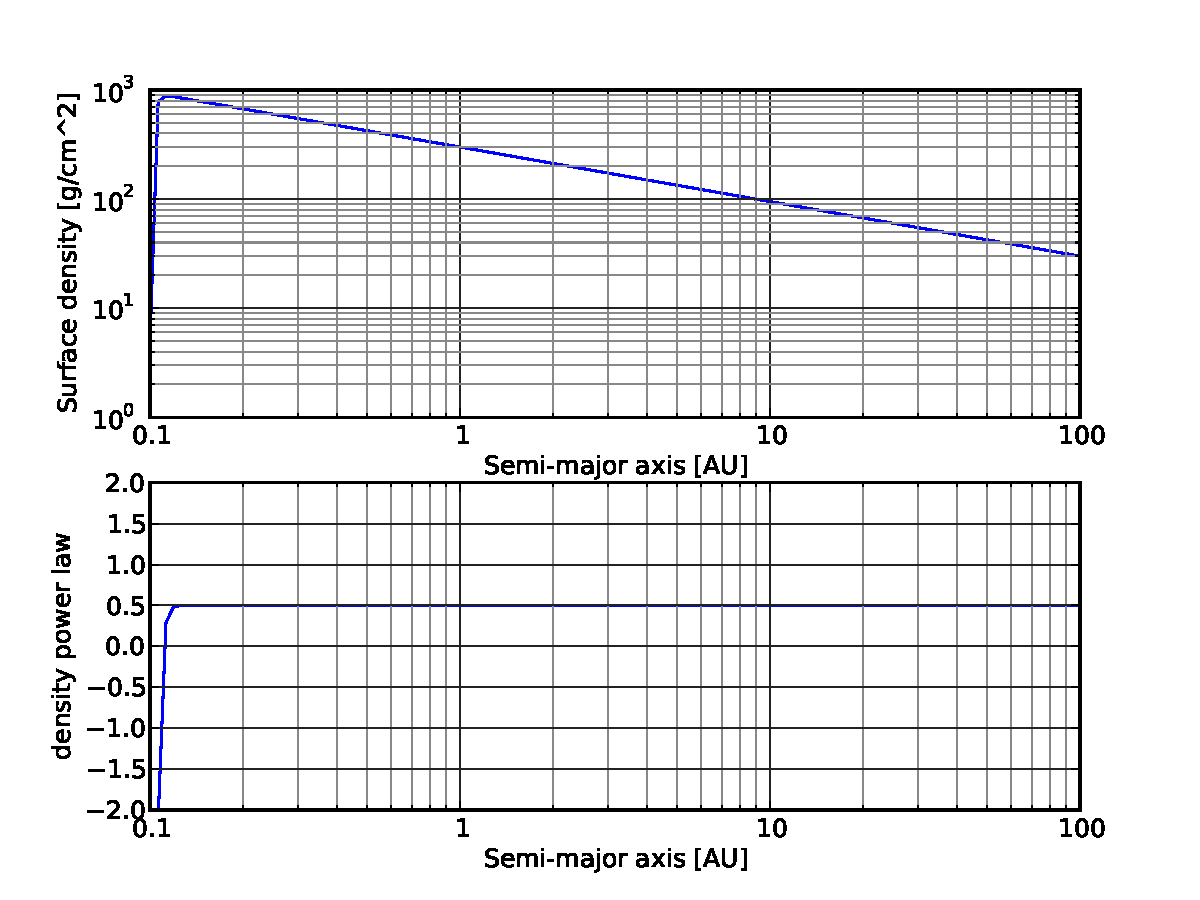
\includegraphics[width=0.75\linewidth]{figure/fiducial_density_profile.pdf}
\caption{Profil de densité de surface pour notre disque de référence \protect\reftab{tab:fiducial_parameters}.}\label{fig:fiducial_density}
\end{figure}

\subsection{Table d'opacité}\index{opacité}
Afin de pouvoir calculer le profil de température, on a besoin de choisir un modèle pour l'opacité. Je ne détaillerai pas ici les différents modèles car une étude spécifique a été menée \refsec{sec:influence_opacity_table} afin de comprendre l'influence du choix du modèle sur les résultats des simulations. 

Par contre, quel que soit le modèle, on a généralement une dépendance en fonction de la densité et de la température. L'opacité est donc un paramètre de la résolution de l'équation qui nous permet d'avoir la température. L'opacité n'est pas, dans notre modèle, une quantité qu'on fixe \emph{a priori}, mais plutôt un des paramètres de sortie de la résolution de l'équation de l'énergie dans le disque.

\subsection{Profil de température}
Afin de construire le profil de température point par point, on résout, pour chaque position dans le disque définie dans le profil, l'équation de l'énergie \refeq{eq:equation_energie}. 

De manière consistante, cette équation a pour paramètre d'entrée la position, et on cherche à trouver les valeurs de la température $T$, échelle de hauteur $H$, profondeur optique $\tau$, diffusivité thermique $\chi$. Toutes ces valeurs sont fixées une fois qu'un ensemble cohérent de valeurs satisfont l'équation.

Afin de résoudre cette équation du type $f(x)=0$, j'ai utilisé une version modifiée de la routine \textbf{zbrent} de \textbf{Numerical Recipes} \citep{press1992numerical}. Cette routine utilise la méthode de Van Wijngaarden-Dekker-Brent. Cette méthode est une combinaison de plusieurs méthodes et permet d'assurer la convergence tout en étant relativement rapide.

Le profil de température que nous obtenons dans notre disque de référence (dont nous parlerons plus en détail \refsec{sec:migrations-maps}) est représenté \reffig{fig:fiducial_temperature}

\begin{figure}[htbp]
\centering
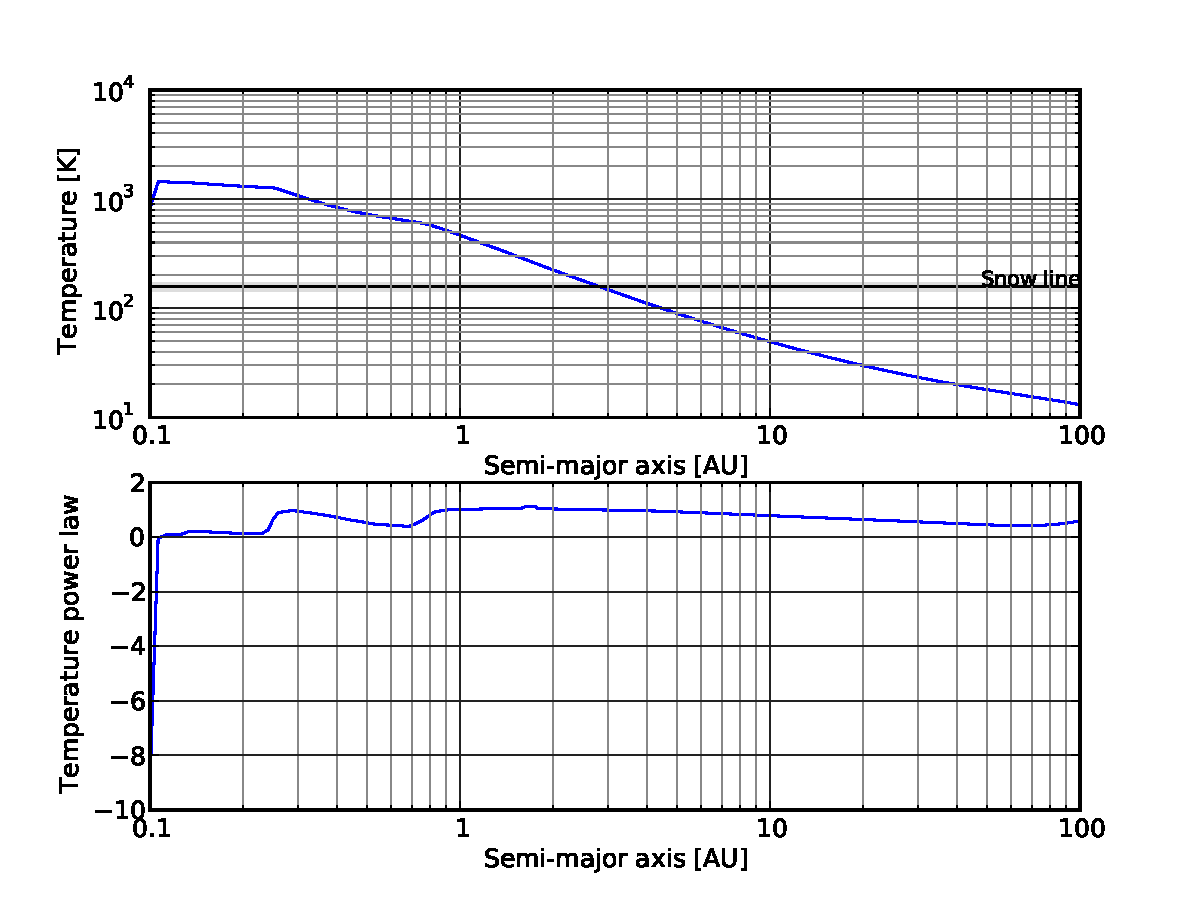
\includegraphics[width=0.75\linewidth]{figure/fiducial_temperature_profile.pdf}
\caption{Profil de température pour notre disque de référence \protect\reftab{tab:fiducial_parameters}.}\label{fig:fiducial_temperature}
\end{figure}

\section{Migration de Type I}\index{migration!Type I}
La migration de Type I est implémentée dans le code en utilisant le modèle 1D de disque, qui définit pour toute position du 
disque, une température, une densité de surface, et tous les autres paramètres nécessaires comme l'échelle de hauteur. En 
utilisant ces paramètres, on obtient ainsi le couple qu'exerce le disque sur la planète en fonction de sa masse et de sa 
position via la formule semi-analytique de \cite{paardekooper2011torque}. Plus exactement, j'implémente les formules décrites 
\refsec{sec:type_I}, équations \refeq{eq:lindblad-torque}, \refeq{eq:saturated-corotation-torque} et 
\refeq{eq:linear-corotation-torque}. Ces formules sont une combinaison de \cite{paardekooper2010torque} où l'effet du paramètre 
de lissage $b/h$ apparaît de manière explicite, mais qui ne modélise que les couples linéaires, et \cite{paardekooper2011torque} 
où l'effet de la diffusion est pris en compte, mais où la longueur de lissage n'apparait pas explicitement. Ainsi, nous 
obtenons des formules pour la migration de Type I qui dépendent du paramètre de lissage $b/h$(\refeq{eq:lindblad-torque}, 
\refeq{eq:saturated-corotation-torque} et 
\refeq{eq:linear-corotation-torque}), et qui en plus tiennent compte 
de la saturation \citep[eqs. (50) à (53)]{paardekooper2011torque}.

Les deux différences principales entre le cadre du modèle de \cite{paardekooper2011torque} et le disque que j'ai modélisé, c'est que dans mon cas je n'ai pas un profil de température en loi de puissance (avec une seule loi de puissance), mais j'ai une loi de puissance définie point par point. C'est-à-dire que pour chaque zone du disque, la température est calculée de manière cohérente avec les autres paramètres du disque, et que l'indice de la loi de puissance correspondante est calculée en fonction des températures autour.

La deuxième différence est que j'ai un profil pour l'échelle de hauteur $H$ et le rapport d'aspect $h=H/R$ du disque au lieu d'avoir un rapport d'aspect constant pour tout le disque.

\bigskip

De plus, certaines erreurs se sont glissées dans ce papier. \cite[appendice A]{bitsch2011range} fait remarquer en particulier qu'il manque un facteur 4 dans l'équation (33). Ainsi, la formule que j'ai utilisé pour calculer la conductivité thermique $\chi$ est :
\begin{align}
\chi &= \frac{16\gamma (\gamma-1) \sigma T^4}{3\kappa \rho^2 H^2\Omega^2}
\end{align}

Il y a aussi une erreur dans l'équation (35) car le disque se refroidit par la surface supérieure et la surface inférieure. Mais comme j'utilise dans mon code une équation de l'énergie \refeq{eq:equation_energie} un peu plus complexe où j'ai tenu compte de ce fait là, cette erreur n'a pas d'incidence sur le calcul du couple.

Les formules nous donnent alors un couple exercé par le disque sur la planète. 

À partir de ce couple, on définit un temps de migration $t_\text{mig}$ comme : 
\begin{align}
t_\text{mig} &= -\frac{J}{\Gamma}
\end{align}
où $J$ est le moment cinétique total de la planète et $\Gamma=\dot{J}$ est le couple total exercé par le disque sur la planète.

L'accélération due à la migration $\vect{a_\text{mig}}$ est alors donnée par\citep[eq. 
(14)]{cresswell2008three} :
\begin{align}
\vect{a_\text{mig}} &= -\frac{\vect{v}}{t_\text{mig}}
\end{align}
où $\vect{v}$ est la vitesse instantanée de la planète.

\section{Amortissement de e et I}
L'amortissement de l'excentricité $e$ et de l'inclinaison $I$ d'une planète plongée dans un disque protoplanétaire est modélisé
dans le code via les formules de \cite[eq. (9), (11) et (12)]{cresswell2008three} : 
\begin{subequations}
\begin{align}
t_e &= \frac{t_\text{wave}}{0.780}\left[1-0.14\left(\frac{e}{H/r}\right)^2 + 0.06 \left(\frac{e}{H/r}\right)^3 + 0.18\left(\frac{e}{H/r}\right)\left(\frac{I}{H/r}\right)^2\right]\\
t_I &= \frac{t_\text{wave}}{0.544}\left[1-0.30\left(\frac{I}{H/r}\right)^2 + 0.24 \left(\frac{I}{H/r}\right)^3 + 0.14\left(\frac{e}{H/r}\right)^2\left(\frac{I}{H/r}\right)\right]\\
t_\text{wave} &= \frac{M_\star}{m_p}\frac{M_\star}{\Sigma_p {a_p}^2}\left(\frac{H}{r}\right)^4{\Omega_p}^{-1}
\end{align}
\end{subequations}

L'amortissement de $I$ est arrêté quand l'inclinaison descend en dessous de $I<5\cdot 10^{-4}\unit{rad}$ afin d'empêcher les planètes d'être parfaitement dans le plan $(x,y)$, essentiellement pour empêcher des problèmes numériques.

\section{Effet de l'excentricité sur le couple de corotation}\index{amortissement!couple de corotation}
Afin de tenir compte d'un effet mis en évidence par \cite{bitsch2010orbital}, une petite modification a été effectuée dans le calcul du couple total $\Gamma$ exercé par le disque sur la planète. 

En effet, il a été montré que l'excentricité d'une planète a une influence sur sa zone fer-à-cheval et par extension, sur son couple de corotation $\Gamma_C$. Un paramètre d'amortissement $D$, compris entre 0 et 1 a ainsi été ajouté au calcul du couple total \citep{hellary2012global} :
\begin{align}
\Gamma &= \Gamma_0 \cdot (\frac{\Gamma_L}{\Gamma_0} + D\cdot \frac{\Gamma_C}{\Gamma_0})
\end{align}
où $\Gamma_0 = \left(\frac{q}{h}\right)^2\Sigma_p {r_p}^4 {\Omega_p}^2$ et $\Gamma_L$ est le couple de Lindblad.

La valeur du paramètre d'amortissement $D$ est donnée par une formule qui a été calculée pour coller au mieux aux simulations de \cite{bitsch2010orbital}, détaillée dans \cite{cossou2013convergence}, et recopiée ici : 
\begin{subequations}
\begin{align}
D = \frac{\Gamma_C(e)}{\Gamma_C (e=0)} &= 1 + a \cdot \left[\tanh(c) - \tanh\left(\frac{b * e}{x_s}+c\right)\right]\label{eq:eccentricity-influence}\\
a &= 0.45 \qquad b=3.46 \qquad c= -2.34
\end{align}
\end{subequations}
où $x_s$ représente la demi-largeur de la région fer-à-cheval adimensionnée.

\section{Désactivation des effets du disque}
Quand une planète sort des bornes du disque, les effets d'amortissement de $e$ et $I$ sont désactivés, au même titre que la migration due à la présence du disque. Ce cas survient rarement au bord externe du disque (généralement à $100\unit{UA}$), mais est beaucoup plus probable au bord interne (généralement à $0.1\unit{UA}$).

\section{Validité des éléments orbitaux}
Lors d'une rencontre proche entre deux planètes, leurs interactions gravitationnelles rendent caduques les formules qui permettent de calculer les éléments orbitaux à partir des vitesses et positions car ceci suppose qu'on est dans le cas d'une orbite képlerienne isolée. 

Dans de tels cas, on peut avoir des demi-grands axes négatifs, des excentricités supérieures à 1. Si c'est déjà en soit un 
problème physique, c'est aussi et surtout un problème numérique car cela fait apparaître des \textbf{Not A Number} (NaN) lorsque 
par exemple le demi-grand axe est en argument d'une racine carrée. Ceci a donc pour conséquence concrète de faire planter le 
code, au mieux, ou pire, de le faire tourner avec tous les paramètres de la simulation peu à peu gangrénés par des 
\textbf{NaN}. 

Dans un premier temps, j'ai pensé remplacer dans mes calculs le demi-grand axe par le rayon $r=\sqrt{x^2+y^2+z^2}$, afin 
d'éviter les problèmes lors des rencontres proches. Cette solution fait apparaître d'autres problèmes, notamment avec des 
orbites excentriques proches du bord interne. Dans ce cas, on peut avoir une planète qui ressent un couple positif au bord 
interne, puis plus de couple du tout dans la partie de l'orbite qui sort du disque, et enfin un couple négatif quand la planète 
est dans le disque, mais hors du bord interne. Ceci cause de gros problèmes et génère des orbites qui ne sont pas physiques 
mais dues à une astuce qui cherche à contourner un problème numérique. En effet, les formules de migration sont moyennées sur 
une orbite, on ne peut donc pas avoir de telles variations au sein d'une même orbite.

La solution adoptée est de tester les cas qui causent des NaN, c'est à dire typiquement des excentricités supérieures à 1, et 
un demi-grand axe négatif. Quand de tels cas surviennent, on désactive momentanément la migration et tous les effets du 
disque. Le reste du temps, la migration est systématiquement calculée, y compris pendant les rencontres proches. On considère 
que le temps durant lequel le calcul des éléments orbitaux n'est plus valide représente un temps négligeable de la 
simulation au regard des centaines de milliers d'années sur lesquelles on intègre les orbites. On considère donc que la 
migration induite sur les planètes pendant les rencontres proches est totalement négligeable au regard du reste de la 
simulation.



\chapter{Mécanismes individuels}
\section{Les Zones de Convergence}
Dans les disques radiatifs, la migration de type I est gouvernée par le couple différentiel de Lindblad, qui induit généralement une migration vers l'intérieur \citep{tanaka2002three}, et le couple de corotation, qui peut contrebalancer le couple différentiel de Lindblad sous certaines conditions et ainsi inverser le sens de migration (vers l'extérieur) \citep{paardekooper2006halting, kley2008migration}. Il est donc possible d'avoir dans un disque des zones où la migration s'arrête. Ces zones sont appelées zone de convergence \citep[CZs;][]{lyra2010orbital, mordasini2011application, paardekooper2011torque}. 

\bigskip

À la zone de convergence, le couple de corotation (positif) compense exactement le couple différentiel de Lindblad (négatif). Ainsi, à la zone de convergence, une planète ne migre pas.

De plus, autour de la zone de convergence, la migration tend à ramener les embryons vers la zone de couple nul s'ils s'en éloignent. La zone de convergence est donc une position stable dans le disque vers laquelle les embryons se rassemblent.

Il peut exister de même des zones de couples nuls qui ne sont pas des zones de convergence quand, en s'éloignant légèrement, la migration tend à les éloigner davantage. Ces zones sont alors instables.

Les zones de convergences pourraient ainsi concentrer les embryons planétaires et être le lieu de formation de planètes (ou cœurs) massives \citep{lyra2010orbital, horn2012orbital}. 

%TODO 
%Je sais pas quoi mettre, mais il faudrait que j'affiche les comparaisons entre les temps particuliers, U-turn et libration ,
% avec les temps de diffusion. 
%TODO 


%TODO 
\subsection{Diagrammes de couple a-m}\label{sec:migrations-maps}
%TODO parler des raisons pour lesquelles la zone de convergence dépend de la masse et de la distance parfois, avec les
%comparaisons des temps (dynamique, de U-turn and de diffusion)

\begin{figure}[htb]
\centering
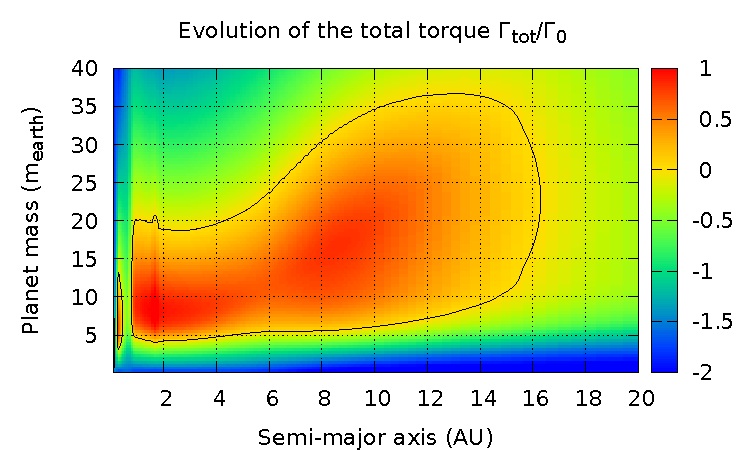
\includegraphics[width=\linewidth]{figure/migration_map/fiducial.pdf}

\caption{Carte de migration pour le disque fiducial. Cette carte montre le sens de migration d'une planète en fonction de sa position (abscisse) et de sa masse (ordonnée). La 3\ieme coordonnée est le couple total exercé par le disque sur la planète, exprimé en unité de $\Gamma_0 = \left(\frac{q}{h}\right)^2\Sigma_p {r_p}^4 {\Omega_p}^2$. Quand le couple est positif (resp. négatif), la migration est vers l'extérieur (resp. intérieur). La ligne noire représente la zone de couple nul, où la planète ne migre plus. Le détail des paramètres du disque de référence est donné \reftab{tab:fiducial_parameters}. }\label{fig:fiducial_migration_map}
\end{figure}

Afin d'étudier la migration dans les disques, il est pratique de regarder une \og carte de migration\fg, comme \reffig{fig:fiducial_migration_map}. Cette carte permet de voir rapidement les parties intéressantes et de prédire l'évolution d'une planète à partir de la position et masse initiales.

\reffig{fig:fiducial_migration_map} montre la carte de migration du disque de référence que nous utiliserons de manière récurrente ici. Ce disque est obtenu à l'aide de la table d'opacité d'\cite{hure2000transition}. Le profil de température est calculé en tenant compte de l'irradiation, avec des paramètres solaires pour la température et le rayon de l'étoile ($T_\star = 5700\unit{K}$ ; $R_\star = 4.65\cdot 10^{-3}\unit{AU}$). L'albédo du disque est pris égal à $0.5$. La viscosité est calculée à partir d'une prescription alpha \citep{shakura1973black}. On considère un disque dont les bords internes et externes sont respectivement à $0.1$ et $100\unit{UA}$. Les autres paramètres du disques sont récapitulés \reftab{tab:fiducial_parameters}. 

\begin{table}[htb]
\centering
\begin{tabular}{|c|c|c|c|}
\hline
$b/h = 0.4$ & $\gamma = 7/5$ & $\mu = 2.35$ & $\alpha = 5\cdot 10^{-3}$ \\\hline
\multicolumn{2}{|c|}{Inner edge : $0.1\unit{UA}$} & \multicolumn{2}{c|}{Outer edge : $100\unit{UA}$}\\\hline
\multicolumn{4}{|c|}{$\Sigma(R) = 300 \cdot R^{-1/2}\unit{g/cm^2}$}\\\hline
$T_\star = 5700\unit{K}$ & $R_\star = 4.65\cdot 10^{-3}\unit{AU}$ & \multicolumn{2}{c|}{Disk albedo : $0.5$}\\\hline
\end{tabular}
\caption{Paramètres physiques du disque fiducial. Les opacités sont calculées à partir de la table d'opacité de \cite{hure2000transition}. La viscosité est calculée en suivant la prescription alpha de \cite{shakura1973black}.}\label{tab:fiducial_parameters}
\end{table}

\begin{figure}[htb]
\centering
\subfloat[Lindblad torque]{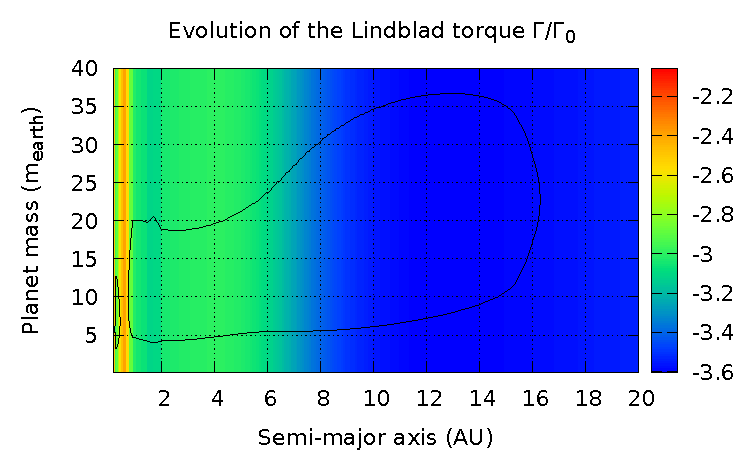
\includegraphics[width=0.49\textwidth]{figure/migration_map/details/lindblad_torque.pdf}}\hfill
\subfloat[Horseshoe Entropy related torque]{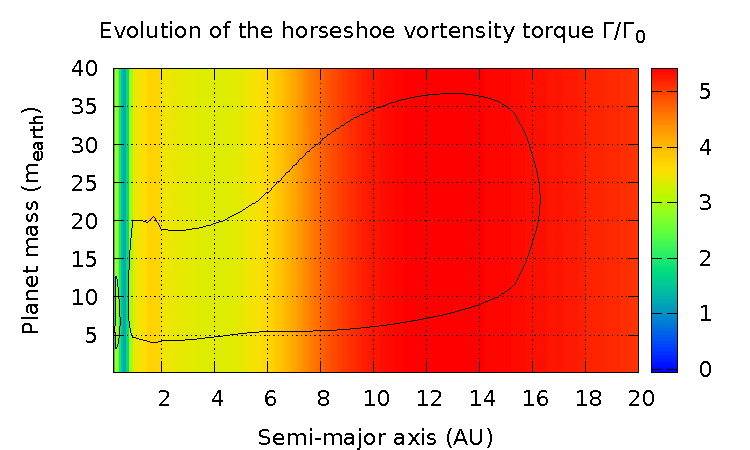
\includegraphics[width=0.49\textwidth]{%
figure/migration_map/details/ent_hs_torque.pdf}}

\caption{Evolution des deux couples les plus importants vis à vis de la carte de migration, le couple de Lindblad et la partie non saturée du couple de corotation liée au gradient d'entropie. En effet, ces deux couples sont quantitativement plus grand que tous les autres. Ici, seule la partie non-saturée du couple de corotation est représentée.}\label{fig:details_maps}
\end{figure}

Sur \reffig{fig:details_maps} sont représentés les deux couples les plus importants en terme d'amplitude (tant négative pour le couple de Lindblad $\Gamma_L$, que positive pour la partie du couple de corotation non saturée liée au gradient d'entropie $\Gamma_\text{ent,hs}$. Ici, c'est bien la partie non saturée qui est représentée \og fully unsaturated\fg. On ne tiens pas compte de la diffusion. On constate alors que sans tenir compte de la diffusion, les couples sont totalement indépendants de la masse. La transition que l'on constate dans les deux cartes, entre $6-8\unit{UA}$ correspond à la transition disque actif/passif. L'irradiation est le processus de chauffage principal à partir de $5\unit{UA}$ comme illustré par \reffig{fig:viscous_vs_irradiation}.

\begin{figure}[htb]
\centering
\subfloat[$t_\text{rad}/t_\text{U-turn}$]{\label{fig:linear_rad}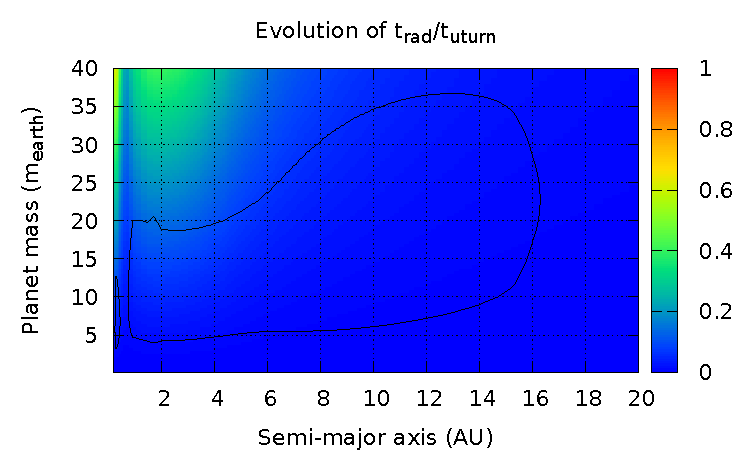
\includegraphics[width=0.49\textwidth]{figure/timescales/linear_rad.pdf}}\hfill
\subfloat[$(t_\text{lib}/2)/t_\text{visc}$]{\label{fig:sat_visc}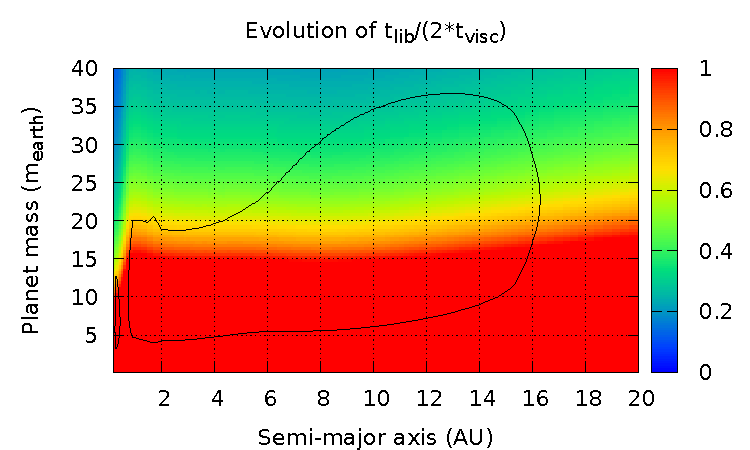
\includegraphics[width=0.49\textwidth]{%
figure/timescales/sat_visc.pdf}}

\caption{Comparaison des différents temps caractéristiques influençant le couple de corotation. Ces inéquations sont détaillées dans \refsec{sec:couple-corotation}. Dans le cas présent, le temps de diffusion radiative est toujours plus court que le temps de diffusion visqueuse, $t_\text{rad}<t_\text{visc}$. Ainsi il ne reste plus que les deux inégalités représentées ici.}\label{fig:timescales_maps}
\end{figure}

\reffig{fig:timescales_maps} représente l'effet de la diffusion sur la carte de migration. Seuls deux cartes sont montrées, contrairement aux quatres que nous pourrions attendre, car $t_\text{rad}<t_\text{visc}$. Ainsi, la double inégalité, qui était scindable en 4 sous-inégalités (deux pour chaque temps de diffusion) devient :
\begin{align}
t_\text{U-turn} < t_\text{diff} < \frac{t_\text{lib}}{2}\\
t_\text{U-turn} < t_\text{rad} < t_\text{visc} < \frac{t_\text{lib}}{2}
\end{align}

À partir de \reffig{fig:timescales_maps} on constate deux choses. La première c'est que la zone de couple nul du bas de la carte de migration, est régie par l'inéquation $t_\text{U-turn} < t_\text{rad}$ \reffig{fig:linear_rad}. C'est surtout visible dans la partie $0-4\unit{UA}$ où l'irradiation ne domine pas encore le profil de température. En dessous de cette ligne, c'est uniquement la partie linéaire du couple de corotation qui subsiste. Le temps de diffusion radiatif $t_\text{rad}$ est trop court pour que la zone fer-à-cheval induise une variation des propriétés du disque lors du demi-tour devant la planète. 

La partie supérieure de la carte, quant à elle, est due à la saturation du couple de corotation, illustrée par l'inégalité $(t_\text{lib}/2) > t_\text{visc}$ qui doit être vérifiée pour que le couple ne sature pas \reffig{fig:sat_visc}. Comme précédemment, au delà de $4\unit{UA}$ l'irradiation domine peu à peu le bilan énergétique du disque, et dilate la zone en masse pour laquelle une planète ressens un couple positif.

\begin{figure}[htb]
\centering
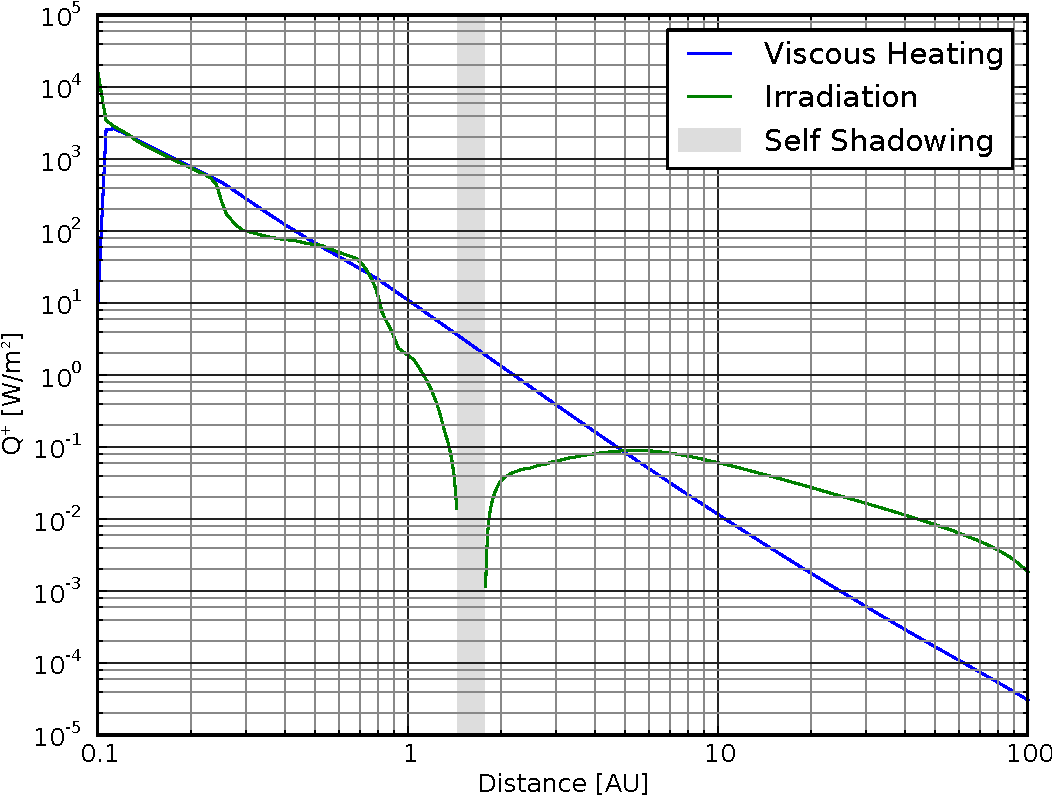
\includegraphics[width=0.75\textwidth]{figure/migration_map/viscous_vs_irradiation.pdf}

\caption{Évolution du chauffage visqueux et de l'irradiation en fonction de la distance. Dans les parties internes, c'est le chauffage visqueux qui domine. Dans les parties externes c'est l'irradiation. À $5\unit{UA}$ les deux contributions sont équivalents.}\label{fig:viscous_vs_irradiation}
\end{figure}

\reffig{fig:viscous_vs_irradiation} montre qu'au delà de $5\unit{UA}$ l'irradiation domine le bilan énergétique du disque. Cela correspond à la distance à laquelle les cartes mettant en jeu les temps de diffusions n'expliquent plus la forme de la carte de migration. À partir de cette distance là, l'irradiation dilate la carte de migration

Intéressons nous maintenant aux zones qui ferment verticalement les lignes de couple nul. Dans les parties externes, après $15\unit{UA}$, c'est la conjonction des deux processus de diffusion qui \og ferme\fg le profil de couple. Pour les masses faibles, en dessous de $15-20\mearth$, la migration vers l'intérieur est dur au fait que $t_\text{U-turn} > t_\text{rad}$, c'est alors la valeur linéaire du couple de corotation qui prévaut. Pour les masses plus importantes, le couple de corotation sature car $(t_\text{lib}/2) < t_\text{visc}$. 

Avant $1\unit{UA}$, les deux régions de couples positifs sont séparés. C'est une transition d'opacité à $1\unit{UA}$ environ qui en est la cause, et qui change brusquement les couples de migration, quelle que soit leur origine \reffig{fig:details_maps}. Ce brusque changement d'opacité et de température est la raison de la séparation de la zone de couple positif en deux. Ainsi, les raisons valables à $15\unit{UA}$ le sont ici aussi, mais la variation du couple en fonction de la distance est beaucoup plus grande, de sorte que la position de la zone de convergence semble ne pas dépendre de la masse, contrairement aux parties externes de la carte de migration.

\subsection{Différents types de zone de convergence}\label{sec:CZ-types}
En fonction de la distance, nous pouvons définir des masses critiques extrémales au delà desquelles la migration vers l'extérieur est impossible en raison du temps de diffusion qui est soit trop grand (saturation) soit trop petit (couple linéaire) pour qu'un couple de corotation non saturé puisse exister.

Mais l'information la plus importante de ces cartes de migration est certainement l'évolution du couple en fonction de la distance. Nous pouvons dégager deux types particulier de zones de convergence. 

Le premier type de zone de convergence est ce que nous appellerons une zone de convergence indépendante de la masse. C'est une zone qui se trouve plutôt dans les parties interne du disque. Cette ligne de couple nul dépend très peu de la masse de la planète car une transition d'opacité induit de brusques changements de température. Les couples varient ainsi fortement sur une distance très courte. Cette zone de convergence a deux caractéristiques importantes : 
\begin{enumerate}
\item La position de la zone de convergence ne dépend pas ou peu de la masse de planète
\item La variation du couple de migration autour de la zone de convergence est très forte
\end{enumerate}

Nous pouvons appeler le deuxième type \og zone de convergence dépendant de la masse\fg. En effet, dans les parties externes, le couple varie plus doucement en fonction de la distance. L'influence de la masse est donc plus marqué dans la position de la zone de couple nul. Ce type de zone de convergence a deux caractéristiques importantes : 
\begin{enumerate}
\item La position de la zone de convergence dépend de la masse de la planète. 
\item Le couple de migration varie doucement en fonction de la distance à la zone de convergence
\end{enumerate}

\begin{figure}[htb]
\centering
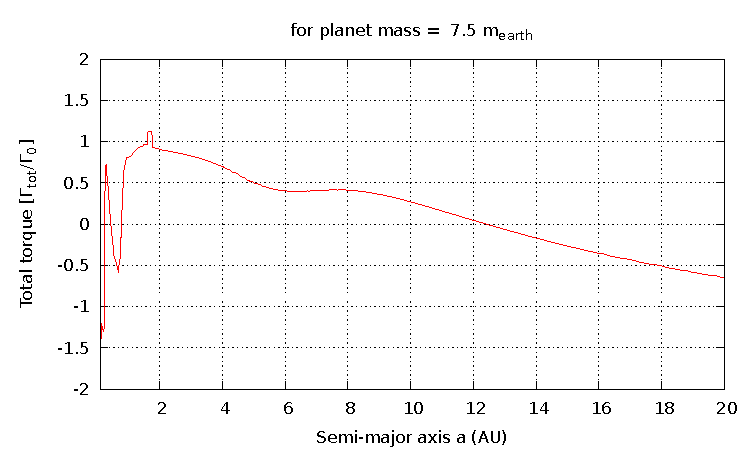
\includegraphics[width=0.75\linewidth]{figure/total_torque_fixed_m.pdf}
\caption{Évolution du couple total exercé par le disque sur une planète de $7.5\mearth$. }\label{fig:total_torque_fixed_m}
\end{figure}

\reffig{fig:total_torque_fixed_m} illustre les deux zones de convergences. La première près de $1\unit{UA}$, siège d'une variation brutale du couple de migration, et la deuxième (dont la position dépend de la masse de la planète) où la variation du couple de migration est continue. 

Dans la suite, nous avons parfois utilisé des zones de convergences artificielles afin de simplifier les effets, et d'étudier plus facilement un phénomène particulier. Dans le cas d'une transition d'opacité, nous avons modélisé les zones de convergence indépendantes de la masse par une tangente hyperbolique dont le zéro se situe à la zone de convergence, et où le couple de migration (positif ou négatif) sature très loin de la zone de convergence \refsec{sec:tanh_indep}. Pour modéliser une zone de convergence indépendante de la masse où le couple varie peu autour de la zone de convergence, nous avons utilisé une variation linéaire du couple de migration \refsec{sec:linear_indep}.

Les zones de convergence dépendantes de la masse peuvent être approximées par une variation linéaire de la position de la zone de couple nul en fonction de la masse. Le couple de migration varie quant à lui linéairement en fonction de la distance \refsec{sec:mass_dependant}. 


\section{Les Résonances de Moyen Mouvement (MMR)}
\subsection{Définition}\index{résonance!de Moyen Mouvement}\index{Mean Motion Resonance|see{résonance}}
Les \gras[resonance@résonance]{résonances de moyen mouvement} sont des configurations orbitales particulières de deux planètes
dans lesquelles il existe un lien entre les périodes orbitales des planètes. Exemple, si deux planètes sont en résonance
\MMR{3}{2}, ça signifie que la planète interne effectuera 3 orbites pendant que la planète externe en effectuera 2.

Ces configurations particulières confèrent une stabilité accrue aux planètes. Plus la résonance est forte et plus il sera difficile pour les planètes d'en sortir.

\bigskip

On met généralement une résonance sous la forme \MMR{(p+q)}{p} où $p$ et $q$ sont des entiers. Cette forme permet de mettre en
évidence un des paramètres qui permet de rendre compte de la force de la résonance. En effet, plus $q$ est petit et plus la
résonance est forte. Ainsi, les résonances d'ordre 1 ($q=1$) sont les plus fortes. On dit que $q$ est l'ordre de la résonance
(plus l'ordre est petit et plus la résonance est forte). De même, $p$ est le degré de la résonance.

\begin{attention}
Mais ce n'est pas le seul paramètre à prendre en compte pour évaluer la force d'une résonance et je suis bien incapable de tous les décrire.
\end{attention}

Pour une résonance \MMR{(p+q)}{p} on définit un certain nombre d'angles $\theta_i$ dits \gras[angle de résonance]{angles de
résonance} de la forme :
\begin{align}
\theta_{i+1} &=(p+q)\lambda_2 -p\lambda_1 - \left[i\varpi_{1} + (q-i)\varpi_2\right]
\end{align}
avec $i$ allant de $0$ à $q$ ; où $\lambda$ sont les longitudes moyennes, $\varpi$ les longitudes du péricentre et les indices
$1$ et $2$ se réfèrent respectivement à la planète interne et externe. Pour une résonance \MMR{(p+q)}{p} on a donc $q+1$ angles
de résonance.

Les angles de résonances mesurent l'angle entre les deux planètes au point de conjonction. Si un seul de ces angles est en libration (oscillation autour d'une valeur moyenne) au lieu de circuler librement de $0$ à $2\pi$ alors on dit que les planètes sont en résonances. Le nombre d'angles en libration permettra aussi d'avoir une idée de la force de la résonance.

\begin{exemple}
Soit une résonance \MMR{7}{2}, les angles de résonances sont :
\begin{align*}
\theta_1 &= 7 \lambda_2 -2\lambda_1 - 5 \varpi_1\\
\theta_2 &= 7 \lambda_2 -2\lambda_1 - \left( 4 \varpi_1 + 1\varpi_2 \right)\\
\theta_3 &= 7 \lambda_2 -2\lambda_1 - \left( 3 \varpi_1 + 2\varpi_2 \right)\\
\theta_4 &= 7 \lambda_2 -2\lambda_1 - \left( 2 \varpi_1 + 3\varpi_2 \right)\\
\theta_5 &= 7 \lambda_2 -2\lambda_1 - \left( 1 \varpi_1 + 4\varpi_2 \right)\\
\theta_6 &= 7 \lambda_2 -2\lambda_1 - 5 \varpi_2
\end{align*}
\end{exemple}

\begin{remarque}
Les \gras[kirkwood@Kirkwood!lacunes de]{lacunes de Kirkwood} font elles aussi intervenir des résonances mais contrairement à ce qu'on pourrait penser, ces résonances avec Jupiter sont des zones déplétées en astéroïdes. 

La résonance imposte une valeur de $a$, mais des échanges sont possibles entre les deux corps en résonance et il est possible que par ce biais l'excentricité puisse augmenter, et ainsi dépléter la lacune de kirkwood en favorisant les collisions entre les objets en résonance et les autres qui sont dans la ceinture.
\end{remarque}


%TODO MMR : lire a thorough analysis of the dunamics involved the reader should consult (Murray & Dermott, 1999)
%TODO cité depuis chapitre 8 resonant perturbations : 
% useful reviews of the subject, particularly in the context of orbital evolution through resonance, have been given by Greenberg (1977), Peale (1986) and Malhotra (1988).
%TODO 
\subsection{Résonances et excentricité}
Cela dépend de l'ordre et du degré de la résonance, mais les perturbations gravitationnelles mutuelles de deux corps en résonance de moyen mouvement engendrent des modifications des éléments orbitaux de ces derniers. 

En particulier, l'excentricité de deux corps en résonance a tendance à varier augmenter au cours du temps \citep[eq. (8.29)]{murray2000solar}. 

Nous n'allons pas détailler ici le fonctionnement précis des résonances. Plusieurs auteurs traitent de ce sujet \citep{greenberg1977orbit, peale1986orbital, malhotra1988phd}. C'est un sujet extrêmement complexe, que je ne maitrise absolument pas dans les détails. De plus, dans le cadre de notre étude de la formation des planètes, nous sommes dans un cas un peu différent. Les résonances entre planète ont lieu dans un système dissipatif, le disque protoplanétaire, qui agit sur les éléments orbitaux, par exemple en amortissant l'excentricité et l'inclinaison des planètes.

Il est difficile de prendre pour exemple les cas N-corps classiques et essayer de les appliquer dans le disque de gaz. Dans notre cas, l'amortissement de $e$ et $I$ par le disque stabilise les résonances, empêchant les résonances normalement instables de se briser. Bien entendu, les résonances se brisent dans nos systèmes en formation, mais dans des cas beaucoup plus extrêmes, notamment quand on a une chaîne de résonance contenant plusieurs corps, tous en résonance. 

\subsection{Stabilité et ordre des résonances}
\reffig{fig:MMR_statistique} montre l'influence du degré de la résonance sur l'excentricité des deux planètes mises en jeu. On
constate tout d'abord que sur 250 simulations effectuées, aucune ne présente des résonances d'ordre $q\neq 1$. Dans le cas de la
migration, où les planètes veulent sortir de la résonance au travers de leur migration différentielle, seules les migration
d'ordre 1 sont assez fortes pour survivre. 


\begin{figure}[htb]
\centering
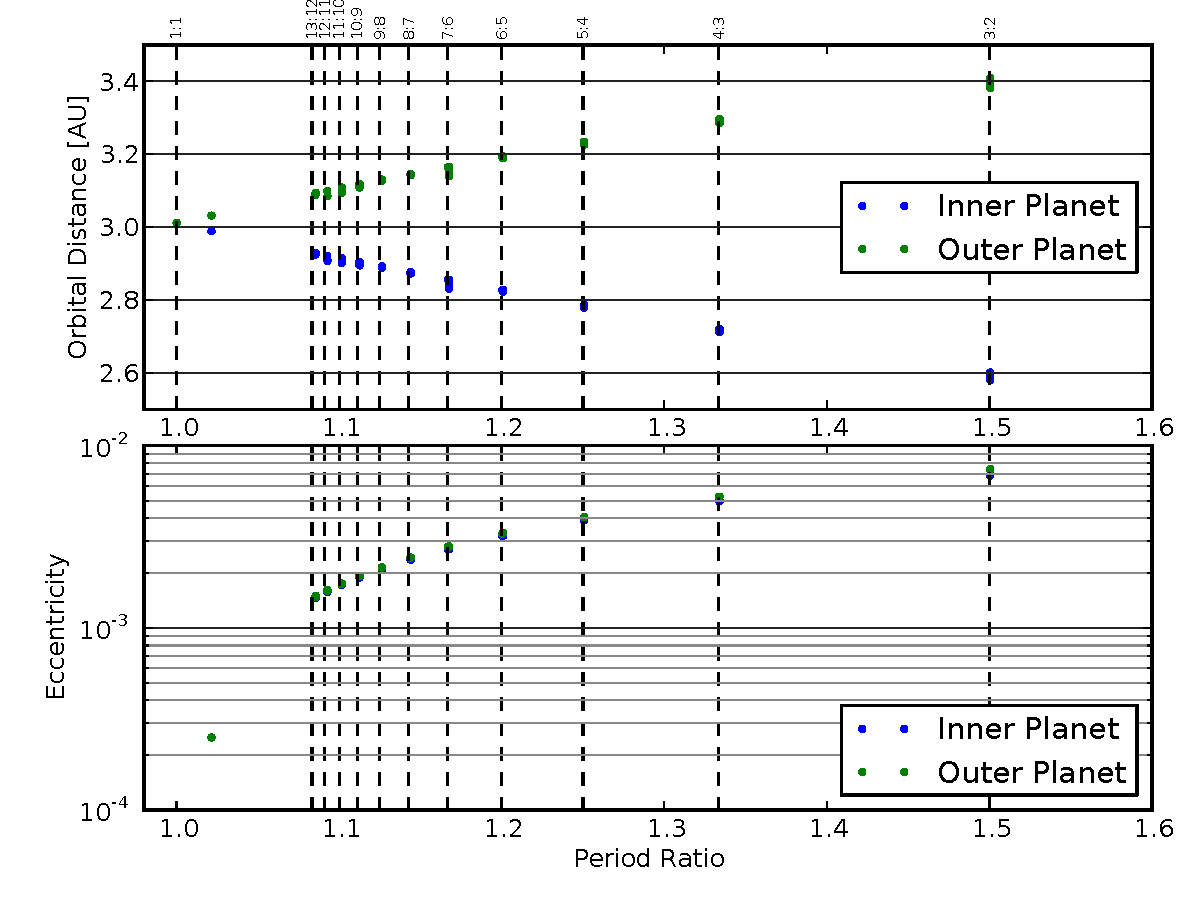
\includegraphics[width=0.75\linewidth]{figure/MMR_statistique.pdf}
\caption{Illustration des différentes résonances possibles et de l'augmentation de l'excentricité qu'elles entrainent. Chaque
simulation contenait deux planètes de $1\mearth$ aléatoirement réparties entre $1$ et $10\unit{AU}$. Chaque point correspond à
une planète. En haut, en fonction du rapport de période, la position finale des planètes est
représentée. En bas, l'excentricité des planètes en fonction du rapport de période avec l'autre planète du système. Une zone de
convergence artificielle à $3\unit{UA}$ a été appliquée. Elle n'a pas d'importance particulier sinon de permettre la formation
de résonances, centrées autour de la même zone du disque, facilitant les études comparatives.}\label{fig:MMR_statistique}
\end{figure}

En fonction du degré de la résonance, l'excentricité des deux corps en résonance diffère. Contrairement à ce qu'on pourrait
penser, ce ne sont pas les résonances de degré élevés qui engendrent les excentricités les plus grandes, même si la distance
entre les deux corps diminue drastiquement. Ainsi, l'excentricité de deux corps sera plus grande s'ils sont en résonance
\MMR{3}{2} par rapport à une \MMR{9}{8}. Ceci vient du fait que même si les planètes sont plus éloignées, dans le cas d'une
résonance \MMR{3}{2}, les conjonctions à l'origine des perturbations gravitationnelles résonances sont beaucoup plus
fréquentes. L'augmentation de l'excentricité est donc beaucoup plus importante \citep{murray2000solar}. 

\subsection{Effet du rapport de masse}
%phd/MMR_mass_ratio
\begin{figure}[htb]
\centering
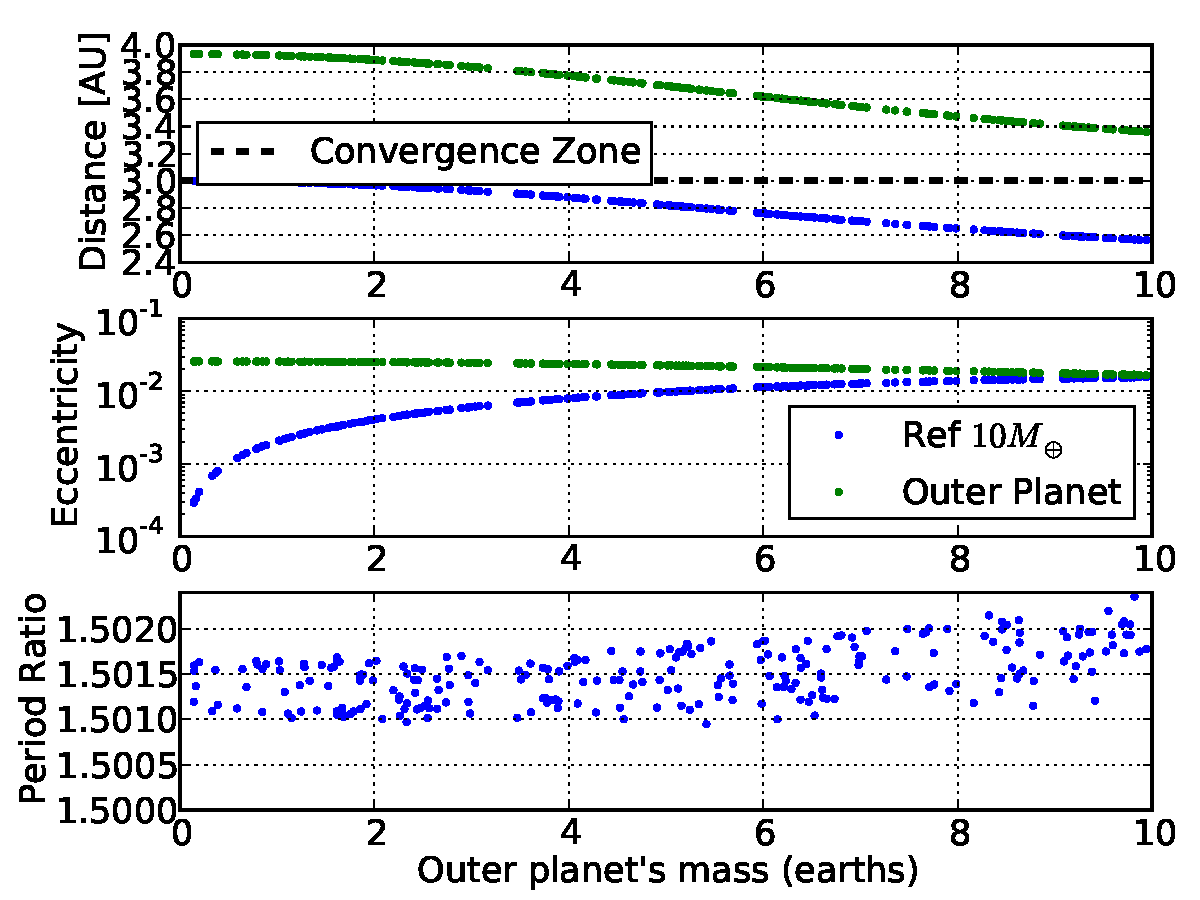
\includegraphics[width=0.75\linewidth]{figure/MMR_mass_ratio.pdf}
\caption{Résultat de 250 simulations où la première planète, de $10\mearth$ est à $3\unit{UA}$, sur
la zone de convergence artificielle. Une planète externe, placée à $4\unit{UA}$ a une masse
déterminée aléatoirement entre $0.1$ et $10\mearth$. Dans la totalité des simulations, les planètes
se placent en résonance \MMR{3}{2}.}\label{fig:MMR_mass_ratio}
\end{figure}

\reffig{fig:MMR_mass_ratio} se lit de gauche à droite, afin de voir l'effet de l'augmentation de la masse de la planète externe
sur la distance orbitale, l'excentricité et le rapport de périodes orbitales. 

Pour une seconde planète de $0.1\mearth$, on constate que la planète la plus massive se trouve à la position exacte de la
résonance, tandis que la planète externe reste bloquée à $4\unit{UA}$ environ. Les deux planètes ressentent un couple de
migration vers la zone de convergence à $3\unit{UA}$ mais l'inertie de la planète massive est beaucoup plus grande, raison pour
laquelle la planète de $10\mearth$ est à la zone de convergence, la planète de faible masse étant simplement bloquée dans la
résonance. 

On constate de plus qu'en raison de la très grande différence de masse, pour une même résonance l'excentricité des deux
planètes est très différente. La planète la plus massive a une excentricité extrêmement basse, cette dernière étant très peu
sensible aux perturbations de la planète de faible masse. À l'inverse, la planète peu massive est très sensible aux
perturbations de la plus grosse, et son excentricité est bien plus importante, plus de deux ordres de grandeur supérieure.

Pour cette planète externe de $0.1\mearth$ on remarque une dernière chose. Bien qu'en résonance \MMR32, le rapport de période
ne vaut pas exactement $1.5$ comme attendu, mais $1.503$. On retrouve là la divergence du rapport de période pour des
résonances dans un système dissipatifs \citep{batygin2013dissipative}. 

\bigskip

À mesure que l'on augmente la masse de la planète externe, cette dernière pousse petit à petit la planète interne, le rapport
de masse se rapprochant de $1$, elle a peu à peu suffisamment de force pour que l'équilibre des couples de migration se
traduise par une répartition des planètes autour de la zone de convergence. 

Dans le même temps, l'excentricité de la planète interne croit. À mesure que la masse de la planète externe augmente, les
perturbations qu'elle engendre sur l'autre planète augmentent également. Sa masse augmentant, elle devient légèrement moins
sensible aux perturbations de la planète interne et on constate une baisse ténue de l'excentricité de la planète externe. 

Enfin, on remarque que l'écart du rapport de période par rapport à la valeur attendue de $1.5$ pour une résonance \MMR32
augmente avec la masse du deuxième corps. En effet, à mesure que la masse de la planète externe augmente, l'amortissement de
l'excentricité induit par le disque devient plus efficace \citep[eq. (9)]{cresswell2008three}. 

\bigskip

Une fois que le rapport de masse est égal à 1, alors les planètes se placent de part et d'autre de la zone de couple nul, et
les excentricités induites par la résonances deviennent sensiblement égales.

\section{Zones de convergence et Résonances}
%TODO talk about the difference between mass dep and mass indep accretion, in particular the fact that planet of different masses migrate to different position has an influence on the convergent migration. 
% In particular, mass indep with linear migration can be equivalent to mass-indep with steep transition.
%TODO

Nous cherchons à comprendre comment l'accrétion est influencée par une zone de convergence. Cette convergence des embryons planétaire vers une zone préférentielle ne résulte pas en la formation d'une super planète, résultat de la collision de tous les embryons de la zone de convergence \citep{morbidelli2008building, sandor2011formation}. Au lieu de cela, les planètes interagissent entre elles et sont piégées dans des résonances de moyen mouvement. 

\begin{figure}[htb]
\centering
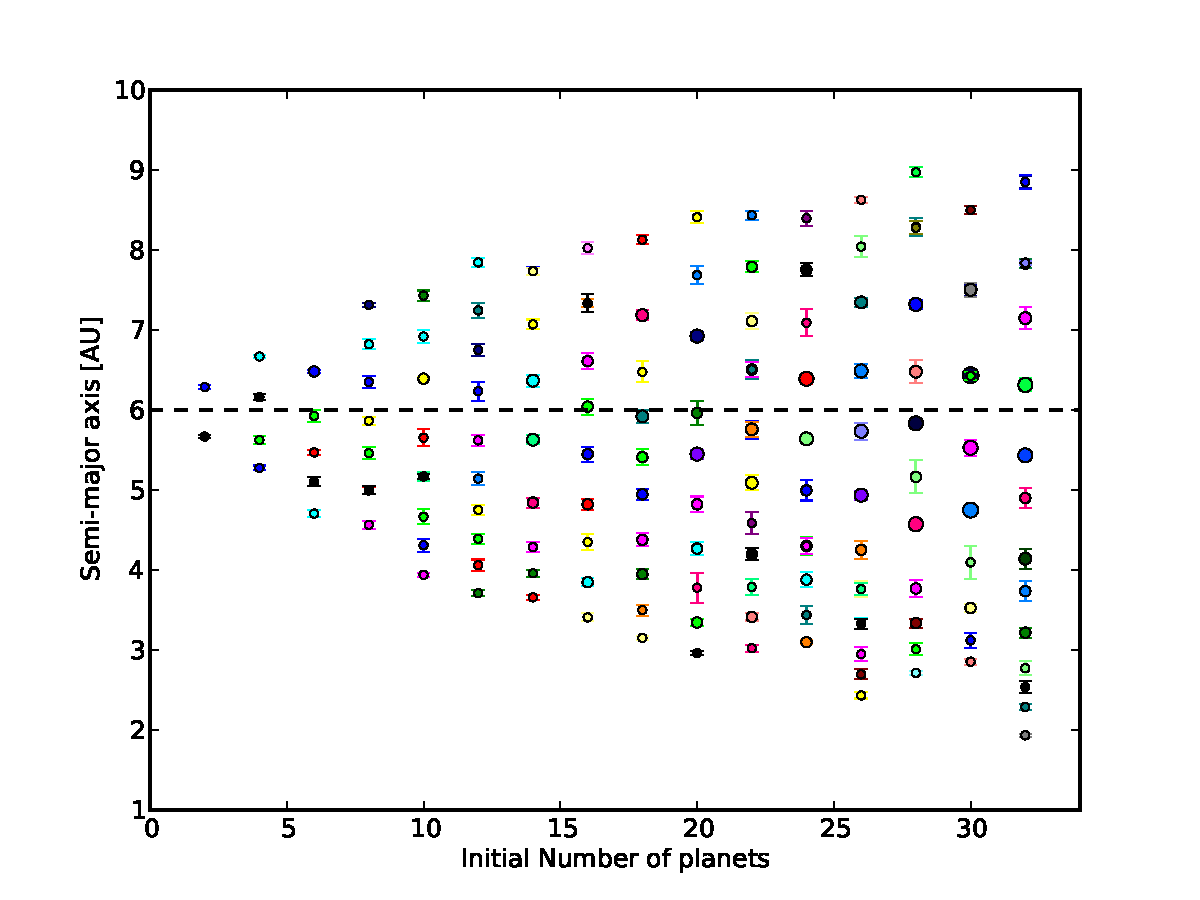
\includegraphics[width=0.75\linewidth]{figure/MMR_number.pdf}
\caption{Stabilisation d'un système planétaire autour d'une zone de convergence artificielle à $6\unit{UA}$ en fonction du nombre de planètes qui le composent initialement. Les eccentricités sont représentées par les barres d'erreurs autour des points symbolisant les planètes, dont le diamètre est proportionnel au rayon (en considérant qu'elles ont toutes la même densité).}\label{fig:MMR_number}
\end{figure}



\chapter{Mécanismes de formation}

\section{Décalage de la Zone de Convergence}\label{sec:shifted_CZ}
Cette partie a fait l'objet d'un article, publié dans le journal Astronomy \& Astrophysics : \cite{cossou2013convergence}.

Une zone de convergence est une zone du disque agissant comme un piège à planète, la migration emmenant les planètes dans cette zone du disque où elles se stabilisent. Ici nous cherchons à montrer que dans le cas multi planétaire, les choses sont un peu différentes. Des planètes en résonance ne se comportent plus de la même manière, mais plutôt comme un système dans sa globalité, migrant dans une zone différente du disque.

\subsection{Introduction}
Des planètes de faible masse ($1-60\mearth$) interagissent avec le disque de gaz dans lequel elles se forment et génèrent des ondes de densité dans le disque \citep{goldreich1979excitation}. La planète elle même est influencée par cette onde de densité et migre par migration de Type I \citep{ward1997protoplanet}.

Dans les disques isothermes, la migration de Type I est gouvernée par le couple différentiel dû aux ondes de Lindblad et le couple de corotation. Pour les planètes, la migration qui en résulte est rapide et dirigée vers l'étoile centrale \citep{tanaka2002three}. Dans les disques radiatifs, un couple lié au gradient d'entropie apparait dans la zone en fer-à-cheval de la planète. Ce dernier peut contrebalancer le couple différentiel de Lindblad au point de transformer la migration vers l'intérieur précédemment présentée en migration vers l'extérieur. Ainsi, dans de tels disques, la migration peut être dirigée soit vers l'intérieur soit vers l'extérieur \citep{paardekooper2006halting, kley2008migration}. Ceci rend possible l'existence de zones dans les disques où la migration s'arrête. Ces dernières sont appelées zone de convergence \citep[CZs;][]{lyra2010orbital, mordasini2011application, paardekooper2011torque}.

\bigskip

À la zone de convergence, le couple de corotation (positif) compense exactement le couple différentiel de Lindblad (négatif). Ainsi, à la zone de convergence, une planète ne migre pas. Les zones de convergences pourraient ainsi concentrer les embryons planétaires et être le lieu de formation de planètes (ou cœurs) massives \citep{lyra2010orbital, horn2012orbital}. 

Cependant, durant leur migration vers la zone de convergence les planètes vont interagir entre elles et se placer en résonance de moyen mouvement (Mean Motion Resonance : MMR), s'opposant ainsi à l'accrétion illimitée de matière à la zone de convergence \citep{morbidelli2008building, sandor2011formation}. Malgré cela, des collisions ont bien lieu à la zone de convergence. Quand les embryons sont emprisonnés dans une chaine de résonance avec suffisamment de corps pour engendrer des perturbations, les résonances peuvent se briser et des collisions se produire entre les corps du système. De plus, la turbulence pourrait casser les résonances et augmenter le taux d'accrétion.

\bigskip

\cite{bitsch2010orbital} ont montré que le couple de corotation était atténué quand une planète avait une excentricité telle que son orbite oscille sur une distance de l'ordre de la demi-largeur de la zone fer-à-cheval $x_s$. 

Quand deux planètes sont en résonance à cause de la migration convergente, leurs excentricités sont excitées de manière continues malgré la présence du disque qui a tendance à amortir les excentricités et circulariser les orbites. \citep[par exemple ][]{cresswell2008three}. Ce phénomène devrait à son tour modifier le couple de corotation et ainsi modifier l'équilibre entre couple différentiel de Lindblad et couple de corotation. En conséquence, la migration de la planète elle-même devrait être modifiée.

\bigskip

Nous présentons des simulations de migration convergentes de planètes de faible masse ($M=1-10\unit{M_\oplus}$) dans un disque de gaz idéalisé (voir \refsec{sec:tanh_indep}). On utilise un modèle simplifié de rétroaction de l'excentricité sur le couple de corotation. Nous montrons que les planètes qui prises de manière isolé migrent à la zone de convergence, ne migrent plus au même endroit quand il y a plusieurs planètes. Au lieu de ça, elles migrent à une position d'équilibre décalée vers l'intérieur du disque qui correspond à une somme nulle des couples exercées sur le système. 

La position de cette zone d'équilibre dépend de l'excentricité maintenue par perturbation mutuelle de chaque planète constituante du système.

\subsection{Méthode}
On modélise une Zone de Convergence (CZ : Convergence Zone) artificielle, qui imite une zone de convergence indépendante de la masse, c'est à dire que la position de la zone de convergence est la même pour toutes les planètes quelle que soit leur masse \refsec{sec:CZ-types}. En particulier, on s'intéresse à la zone de convergence que l'on peut trouver à une transition d'opacité telle que celle représentée sur \reffig{fig:shifted_CZ_torque_prof}, où l'on peut voir un renversement brutal du couple, qui passe de positif à négatif \citep[voir par exemple ][]{masset2011type}.

\begin{figure}[htb]
\centering
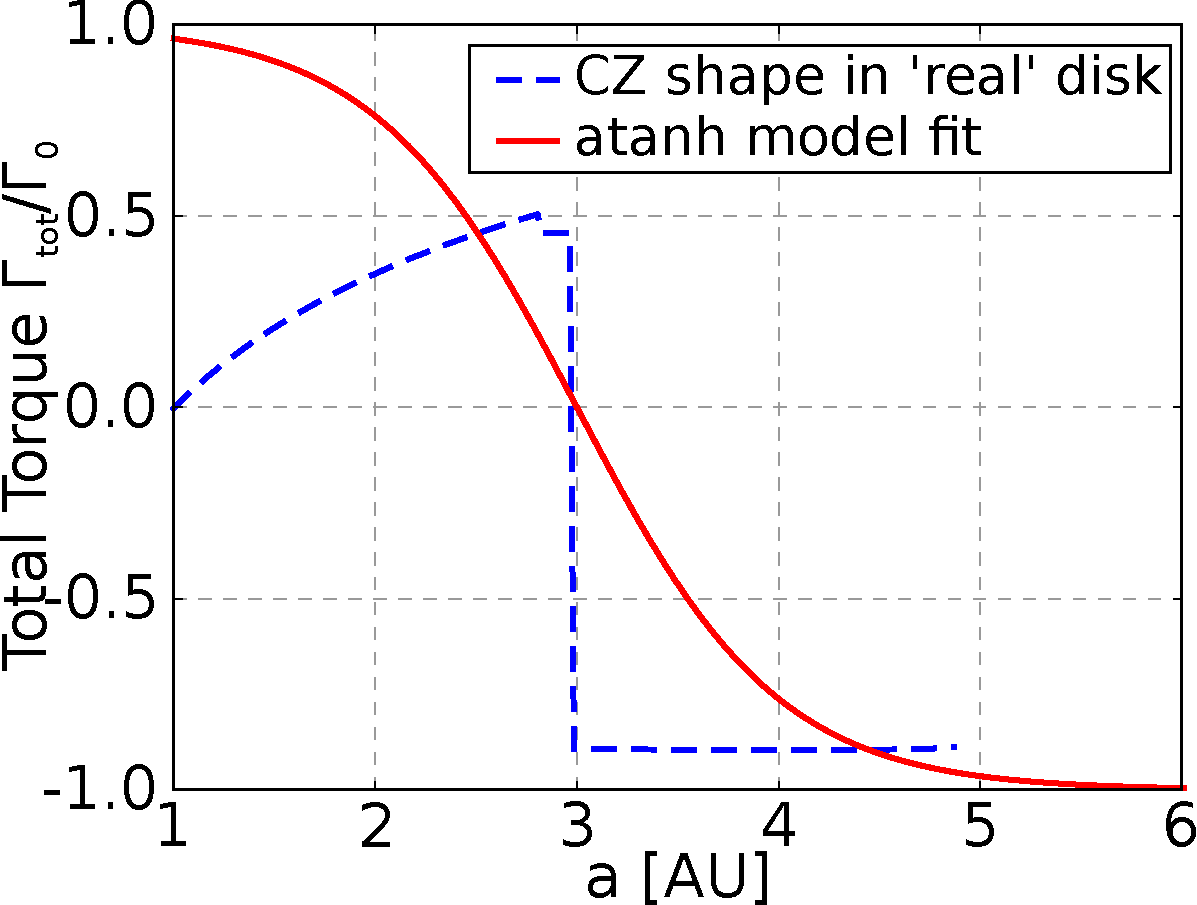
\includegraphics[width=0.49\linewidth]{figure/shifted/torque_zoom_CZ1.pdf}
\caption{Le couple total de notre disque standard est représenté en rouge. La ligne bleue pointillée représente le profil de couple ressenti par une planète de $10\unit{M_\oplus}$ autour d'une transition d'opacité, calculé à partir des équations de \cite{paardekooper2011torque}.}\label{fig:shifted_CZ_torque_prof}
\end{figure}

À noter qu'une fonction de Heavyside n'a pas été utilisée car la marche d'escalier dans le profil \textit{réel} n'est due qu'au fait que la table d'opacité n'a pas été lissée. On s'attend à ce que la transition soit plus douce dans la réalité.
%TODO arnaud veut que je compare une version lissée avec mon tangente hyperbolique.

La position de la zone de convergence était $3\unit{UA}$. À l'intérieur de $3\unit{UA}$, le couple est positif et égal à $\Gamma_0 = \left(\frac{q}{h}\right)^2\Sigma_p {r_p}^4 {\Omega_p}^2$., la migration se fait donc vers l'extérieur. Au delà de $3\unit{UA}$, le couple total est égal à $-\Gamma_0$. Ici $q$ est le rapport entre les masses de la planète et de l'étoile, $h$ est le rapport d'aspect qui dépend du profil de température mais vaut typiquement $0.05$. $\Sigma_p$, $r_p$ et $\Omega_p$ sont respectivement la densité de surface, la distance orbitale et la vitesse angulaire pour la planète. 

Le couple total est la somme du couple différentiel de Lindblad $\Gamma_L$ --- que l'on suppose constant et indépendant de $e$ --- et le couple de corotation $\Gamma_C$. Le principal intérêt de la zone de convergence artificielle est de s'affranchir de la forme très complexe du profil réel et ne garder que la zone de convergence, afin d'en étudier les effets de manière isolée.

\bigskip

\cite{bitsch2010orbital} montrent que la structure de la zone fer-à-cheval est modifiée quand l'excentricité augmente. En conséquence, son couple de corotation $\Gamma_C$, lié à cette région du disque, diminue. 

Nous avons élaboré une formule simple qui reproduit l'effet de l'excentricité sur $\Gamma_C$ par une simple calibration des simulations 3D de \cite{bitsch2010orbital} : 
\begin{align}
D &= \frac{\Gamma_C(e)}{\Gamma_C (e=0)} = 1 + a \cdot \left[\tanh(c) - \tanh\left(\frac{b * e}{x_s}+c\right)\right]\label{eq:shifted-eccentricity-influence}
\end{align}
où $x_s$ représente la demi-largeur de la région fer-à-cheval en unité de distance orbitale de la planète considérée, $e$ est l'excentricité de la planète, et notre ajustement statistique donne les valeurs suivantes pour les paramètres de la fonction :
\begin{align}
a &= 0.45 & b &= 3.46 & c &= -2.34
\end{align}

On défini $x_s$ comme \citep[eq. (44)]{paardekooper2010torque} :
\begin{align}
x_s &= \frac{1.1}{\gamma^{1/4}} \left(\frac{0.4}{b/h}\right)^{1/4} \sqrt{\frac{q}{h}}
\end{align}
où $\gamma$ est l'indice adiabatique, $q$ le rapport entre les masses de la planète et de l'étoile, $h$ le rapport d'aspect et $b/h$ la longueur de lissage du potentiel gravitationnel de la planète (dépendance issue des formules de \cite{paardekooper2011torque}).
%TODO c'est pas uniquement un problème numérique, c'est aussi un problème physique. Voir pour cela paardekooper et papaloizou 2009 ou encore kley & muller 2012
%TODO en gros, de ce que je comprends, il y a le problème de la masse ponctuelle de la planète qui génère une divergence quand on veut calculer la forme des ondes de densité générées par la planète sur le disque. Mais il y a aussi le problème de la longueur de lissage du potentiel du disque quand on veut calculer le couple du disque sur la planète. Il y a donc techniquement deux longueurs de lissages différentes. On doit choisir une seule longueur de lissage pour le potentiel gravitationnel, mais il y a deux longueurs de lissages "optimisées" si on veut faire le calcul d'audrey, JM ou arnaud proprement ; prescription de la longueur de lissage)

\reffig{fig:shifted_CZ_D_profile} montre que notre formule simple \refeq{eq:shifted-eccentricity-influence} correspond bien à la tendance des simulations hydrodynamiques de l'effet de $e$ sur $\Gamma_C$, en particulier pour les excentricités faibles. Il faut tout de même noter qu'il y a peu de points \og expérimentaux\fg et qu'il semble y avoir des fluctuations aléatoires influençant les valeurs mesurées.

\begin{figure}[htb]
\centering
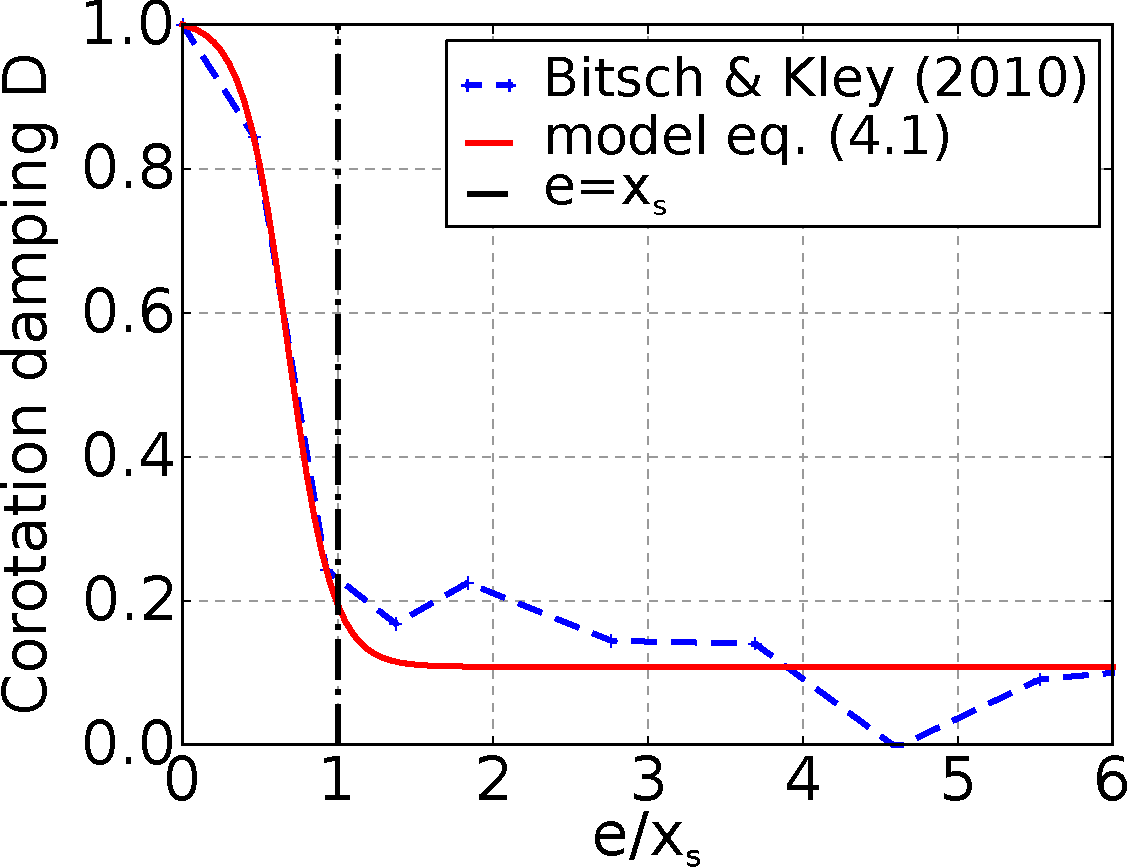
\includegraphics[width=0.49\linewidth]{figure/shifted/corotation_damping_profile.pdf}
\caption{Diminution du couple de corotation $\Gamma_C$ en fonction de l'excentricité $e$. On suppose que l'atténuation ($0<D<1$) du couple de corotation en fonction de l'extencité $e$ est la même dans un disque isotherme ou radiatif. Ainsi, on extrait la valeur de $D$ à partir de la figure 2 de \cite{bitsch2010orbital} en faisant la différence entre la valeur pour le disque radiatif et celle pour le disque isotherme, et normalisant de sorte que $D$ vale $1$ dans le cas $e=0$.}\label{fig:shifted_CZ_D_profile}
\end{figure}

\bigskip

Afin de réaliser nos simulations, nous avons utilisé la version modifiée de l'intégrateur \textbf{Mercury}\citep{chambers1999hybrid} décrite \refsec{sec:code_n-corps}. Nous avons utilisé en particulier la zone de convergence artificielle décrite \reffig{fig:shifted_CZ_torque_prof}. 

Nous supposons que le disque possède le profil de densité de surface suivant :
\begin{align}
\Sigma(R) = 500 \left(R/1\unit{AU}\right)^{-1/2} \unit{g.cm^{-2}}
\end{align}
Ce profil est alors utilisé dans le calcul de $\Gamma_0$ et de l'amortissement induit par le disque sur $e$ et $I$.

Pour implémenter la migration induite par le couple du disque $\Gamma$, on note que $\Gamma=\od{J}{t}$, et on défini une accélération de migration $a_m$ telle que\citep[eq. (14)]{cresswell2008three} :
\begin{align}
a_m &= - \frac{v}{t_m}
\end{align}
où $v$ est la vitesse de la planète et $t_m=J/\od{J}{t}$ le temps de migration ($J$ est le moment cinétique).

\bigskip

Dans toutes les simulations, les planètes était initialement sur des orbites à faible excentricité ($e<0.001$) et faible inclinaison ($I<1^\circ$). Chaque simulation a été intégrée pendant trois millions d'années, avec un pas de temps compris entre $0.4$ et $3$ jours.

\subsection{Le cas de deux planètes}
\reffig{fig:two-planets} montre l'évolution de deux planètes de $1\unit{M_\oplus}$ initialement placées de part et d'autre d'une zone de convergence située à $3\unit{UA}$. Alors qu'elles se rapprochent l'une de l'autre, les deux planètes croisent une série de résonances and finissent piégées dans la résonance \MMR{7}{6}. Les excentricités des deux planètes atteignent alors un équilibre entre excitation résonante et amortissement par le disque. Cette excentricité d'équilibre est environ égale à $0.5$ fois la demi-largeur de la zone fer-à-cheval $x_s$ et amortit le couple de corotation à environ $80\%$ de sa valeur nominale (quand $e=0$). 

\begin{figure}[htb]
\centering
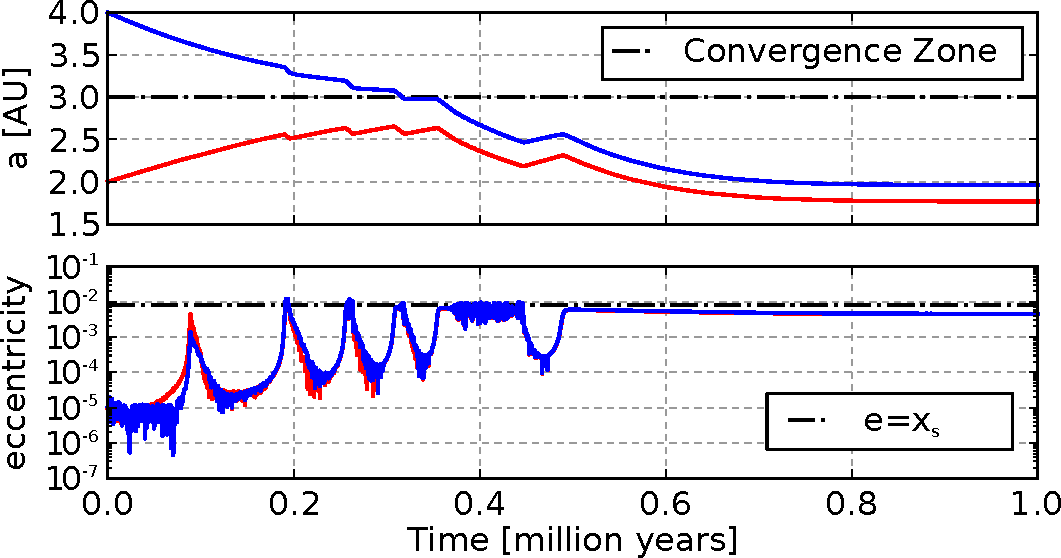
\includegraphics[width=\linewidth]{figure/shifted/corotation_damping_influence.pdf}
\caption{Simulation de la migration convergence de deux planètes de $1\unit{M_\oplus}$ vers la zone de convergence située à $3\unit{UA}$, la rétroactio de l'excentricité $e$ sur le couple de corotation $\Gamma_C$ étant incluse (voir Figure~\ref{fig:shifted_CZ_D_profile}).}
\label{fig:two-planets}
\end{figure}

Les planètes se stabilisent et arrêtent de migrer à $1.77$ et $1.96\unit{UA}$, toutes les deux à l'intérieur de la position nominale de la zone de convergence. Compte tenu de leurs excentricités, la zone de convergence de la planète la plus interne est décalée à $1.95\unit{UA}$ tandis qu'elle est décalée à $1.74\unit{UA}$ pour la planète externe (située à $1.96\unit{UA}$). On constate alors qu'aucune des deux planètes n'est à une position d'équilibre. Chacune d'elle ressent un couple dirigé vers l'autre planète du système, de sorte que la migration tend à rapprocher les planètes tandis que les résonances les maintiennent éloignées.

Le décalage de la zone d'équilibre provient ici de l'équilibre nouveau entre le couple de Lindblad resté inchangé et le couple de corotation atténué par l'excentricité. \emph{Les deux planètes se stabilisent autour d'une zone où le couple total exercé sur le système dans sa globalité est nul, même si chaque planète prise séparément ressent un couple de migration non nul}. Aucune des deux planètes n'est ici à une zone de convergence (même celle calculée en tenant compte de l'atténuation du couple de corotation). 

Il est clair que les excentricités des planètes --- excitées par les interactions entre planètes --- sont le facteur clé pour déterminer la force du couple de corotation et la position effective de la zone de stabilisation du système. Pour deux planètes de même masse, le même comportement qualitatif est observé, quelle que soit la masse ou la résonance considérée : Une plus grande excentricité implique un amortissement plus fort du couple de corotation $\Gamma_C$ et une stabilisation du système de plus en plus proche de leur étoile. 

\subsection{Effet du rapport de masse}\label{sec:mass-ratio-effect}
Nous étudions maintenant le cas de deux planètes de masses différentes. \reffig{fig:mass_ratio_final_pos} représente les positions finales d'une série de simulations simples dans lesquelles une planète de $10\unit{M_\oplus}$ est placée systématiquement à $3\unit{UA}$ en compagnie d'une autre planète, placée à $4\unit{UA}$ et dont la masse varie successivement entre $0.1$ et $3\unit{M_\oplus}$. 

\begin{figure}[htb]
\centering
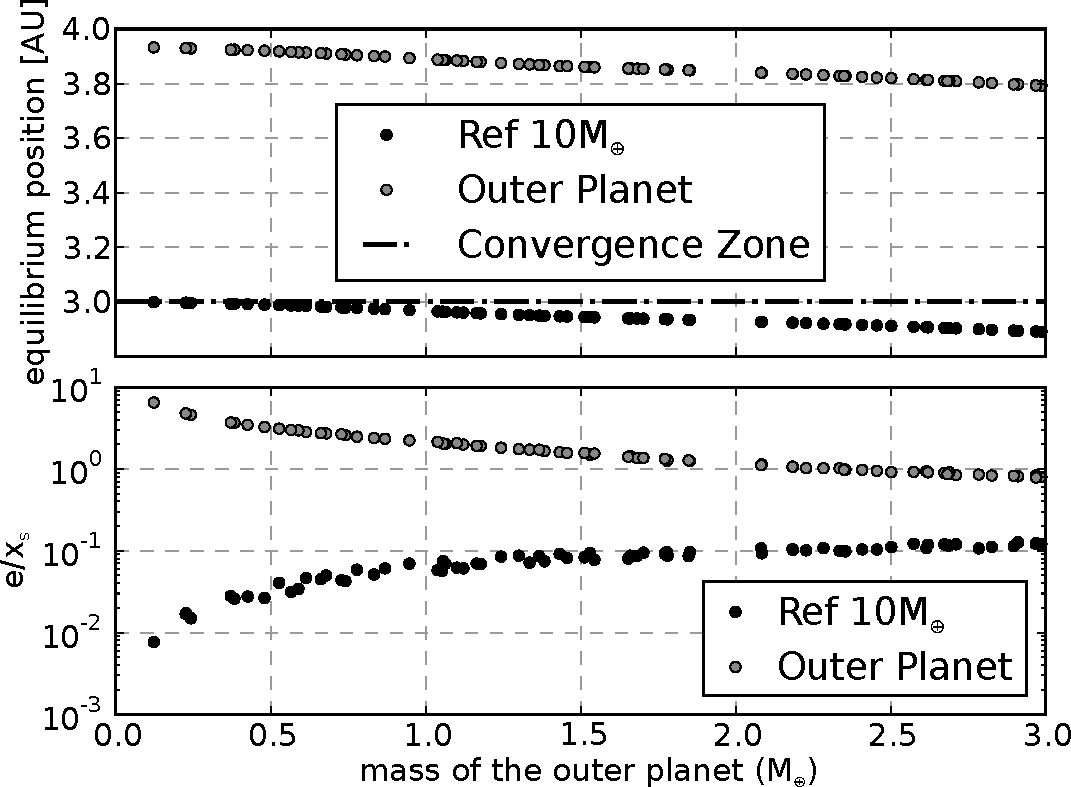
\includegraphics[width=0.95\linewidth]{figure/shifted/mass_ratio_influence.pdf}
\caption{Système final d'une série de simulations avec initialement une première planète à $3\unit{UA}$ de $10\unit{M_\oplus}$ et une deuxième planète à $4\unit{UA}$ dont la masse varie de $0.1$ à $3\unit{M_\oplus}$. Les graphiques montrent la position d'équilibre des planètes (en haut) et les excentricités normalisées par rapport à la demi-largeur de la zone fer-à-cheval $e/x_s$ (en bas) en fonction de la masse de la deuxième planète.}\label{fig:mass_ratio_final_pos}
\end{figure}

\bigskip

Dans \reffig{fig:mass_ratio_final_pos}, la planète externe est systématiquement en résonance \MMR{3}{2} avec la planète interne. Ainsi, la position finale des planètes est déterminée par leur masse respective ou, pour cette expérience, par la masse de la planète externe vu que la masse de la planète interne est fixe. 

Plus la deuxième planète est massive, et plus le décalage du système planétaire par rapport à la zone de convergence est important. En effet, une planète externe plus massive induit une excentricité plus importante pour la planète interne, ce qui correspond à un amortissement plus important de son couple de corotation $\Gamma_C$ et un décalage plus important de la zone d'équilibre du système. Compte tenu du fait que chaque planète possède une masse et une excentricité différentes, elles ressentent une zone de convergence différente (une pour chaque valeur de $e/x_s$). Pour autant, l'importance du décalage vers l'étoile centrale de la position d'équilibre est principalement déterminée par la dynamique de la planète la plus massive et de sa nouvelle zone de convergence.

\bigskip

\reffig{fig:mass_ratio_final_pos} représente uniquement un sous-ensemble de toutes les simulations de cette expérience. Pour des masses plus importantes, les deux planètes étaient dans des résonances différentes, ce qui causait des discontinuités dans le diagramme, rendant difficile sa lecture. Malgré tout, le comportement du système de deux planètes est qualitativement le même.

\subsection{Effet des résonances}
Dans la position d'équilibre d'un système de deux planètes, l'ordre de la résonance entre les deux corps est aussi important (pour une résonance de moyen mouvement \MMR{(p+q)}{p}, $p$ est l'ordre de la résonance). 
%TODO demander à Sean pour ça. Arnaud me dit que l'ordre, c'est q, et que p est le degré de la résonance.

Deux planètes en résonance \MMR{3}{2} auront des excentricités plus importantes que si elles étaient en résonance \MMR{11}{10}. L'explication simple est qu'une résonance d'ordre moins élevé implique des conjonctions plus fréquentes, et ainsi des perturbations plus importantes (voir \cite{murray2000solar} pour plus de détails). La résonance dans laquelle un système de deux planètes se place dépend de la vitesse de migration relative et du taux d'amortissement de l'excentricité par le disque (voir par exemple \cite{mustill2011general}). Ces deux derniers paramètres sont déterminés à la fois par le disque, le profil de couple et les positions initiales des planètes. 

\begin{figure}[htb]
\centering
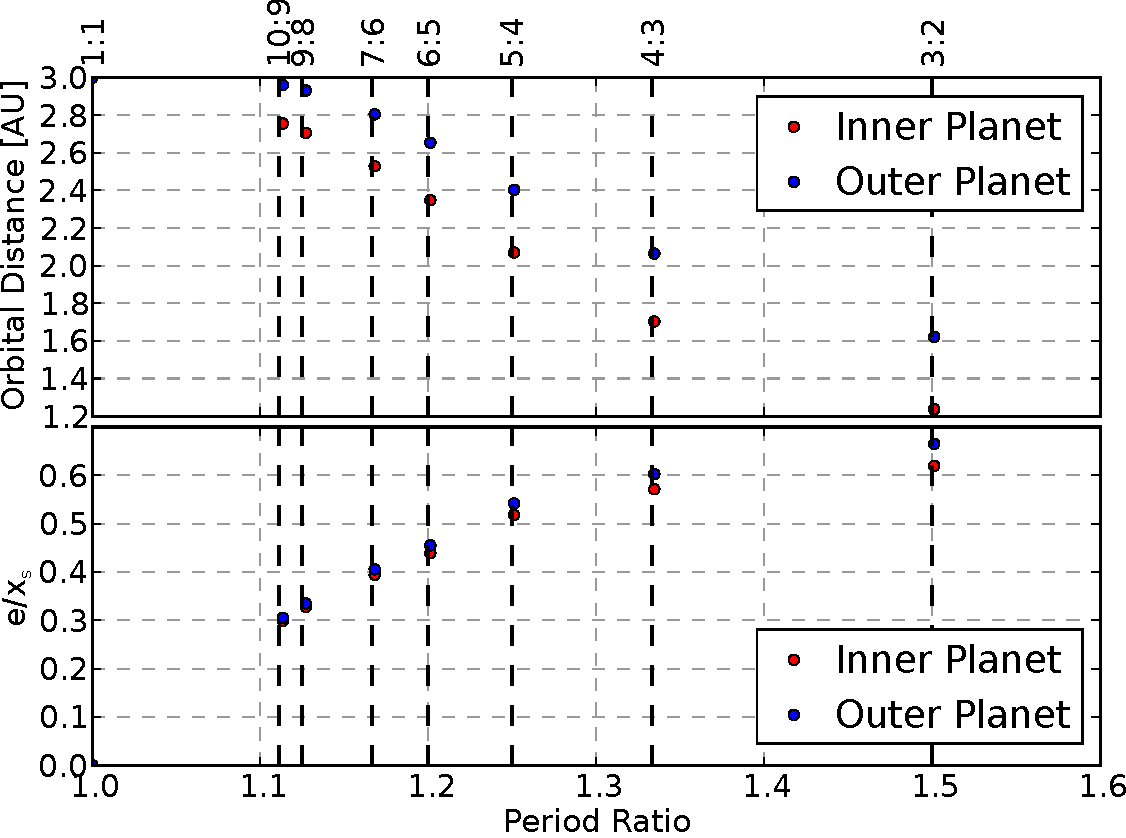
\includegraphics[width=0.95\linewidth]{figure/shifted/influence_of_MMR.pdf}
\caption{demi-grand axe final (en haut) et excentricité (en bas) de deux planètes de $3\unit{M_\oplus}$ piégées dans différentes résonances de moyen mouvement. Pour une planète de $3\unit{M_\oplus}$, la demi-largeur de la zone fer-à-cheval vaut environ $0.014$.}\label{fig:influence_of_MMR}
\end{figure}

Afin de tester l'effet des résonances, nous avons fait une série de 100 simulations (chacune intégrée pour un million d'années), avec deux planètes de $3\unit{M_\oplus}$ placés aléatoirement entre 1 et 10 UA, avec la même zone de convergence artificielle placée à 3 UA que précédemment. 

\reffig{fig:influence_of_MMR} montre que dans tous les cas, les planètes sont bloquées dans des résonances allant de \MMR{11}{10} à \MMR{3}{2} (ordre de la résonance de 10 à 2). Conformément à ce qui était attendu, les excentricités maintenues grâce aux résonances diminuent à mesure que l'ordre des résonance augmente, et ceci induit un décalage moins important du système planétaire par rapport à la zone de convergence à 3 UA. L'amplitude du décalage vers l'intérieur de la position d'équilibre varie de 0.2 à 1.5 UA. 

Dans deux simulations, les planètes ont commencé si proches l'une de l'autre qu'elles se sont retrouvé en résonance co-orbitale (résonance \MMR{1}{1}). Dans ces cas là, leurs excentricités sont restées très faibles, et les deux planètes ont migré en co-orbite jusqu'à la zone de convergence nominale à 3 UA. 

\subsection{Évolution avec plus de deux planètes}
On se concentre maintenant sur le cas multi-planètes. Nous avons lancé 10 simulations pour des cas avec deux, trois, cinq ou dix planètes, initialement toutes de $3\unit{M_\oplus}$. Les planètes étaient placées aléatoirement entre 1 et 10 UA, et étaient sur des orbites de faible inclinaison et excentricité. Comme précédemment, chaque simulation a été intégrée pendant trois millions d'années dans un disque statique (sans dissipation). 

\bigskip

Dans les cas avec 3 planètes, on trouve 3 scénarii différents. Dans un premier cas, les 3 planètes sont prises dans une chaine de résonance et migrent vers l'intérieur toutes ensemble jusqu'à une zone d'équilibre où le couple total exercé sur le système est nul. Cette zone est typiquement entre 2 et 2.5 UA. Les excentricités des trois planètes ne sont pas identiques, la planète au centre de la chaîne de résonance est généralement la plus excitée. 

Dans le deuxième scénario le plus probable, deux planètes entrent en résonance et migrent vers l'intérieur tandis que la troisième et dernière planète est trop loin dans le disque pour être elle aussi prise en résonance avec les deux autres. Cette dernière planète migre alors à la zone de convergence à 3 UA, tandis que les deux planètes internes stoppent leur migration autour d'une zone d'équilibre où le couple total exercé sur le système est nul. 

Enfin, dans un troisième scénario, une collision a lieu et le système revient à un cas à deux planètes de masse différente comme vu précédemment \reffig{fig:mass_ratio_final_pos}. 

\bigskip

Pour les cas à 5 et 10 planètes, la situation est plus complexe. Les systèmes de 5 planètes forment des chaines de résonances et migrent vers l'intérieur, en direction d'une position d'équilibre où le couple total est nul. Cependant, les perturbations entre planètes ajoutent un aspect erratique à la migration des planètes. Même les systèmes les plus stables subissent des périodes d'instabilités durant lesquelles les planètes dérivent radialement dans la même direction. Ces périodes sont déclenchées par la sortie d'une résonance d'un couple de planètes à l'intérieur du système. Cette sortie de résonance se propage alors comme une perturbation à travers tout le système. L'amplitude et la fréquence de ces périodes chaotiques varient d'une simulation à l'autre. 

%\begin{figure}[htb]
%\centering
%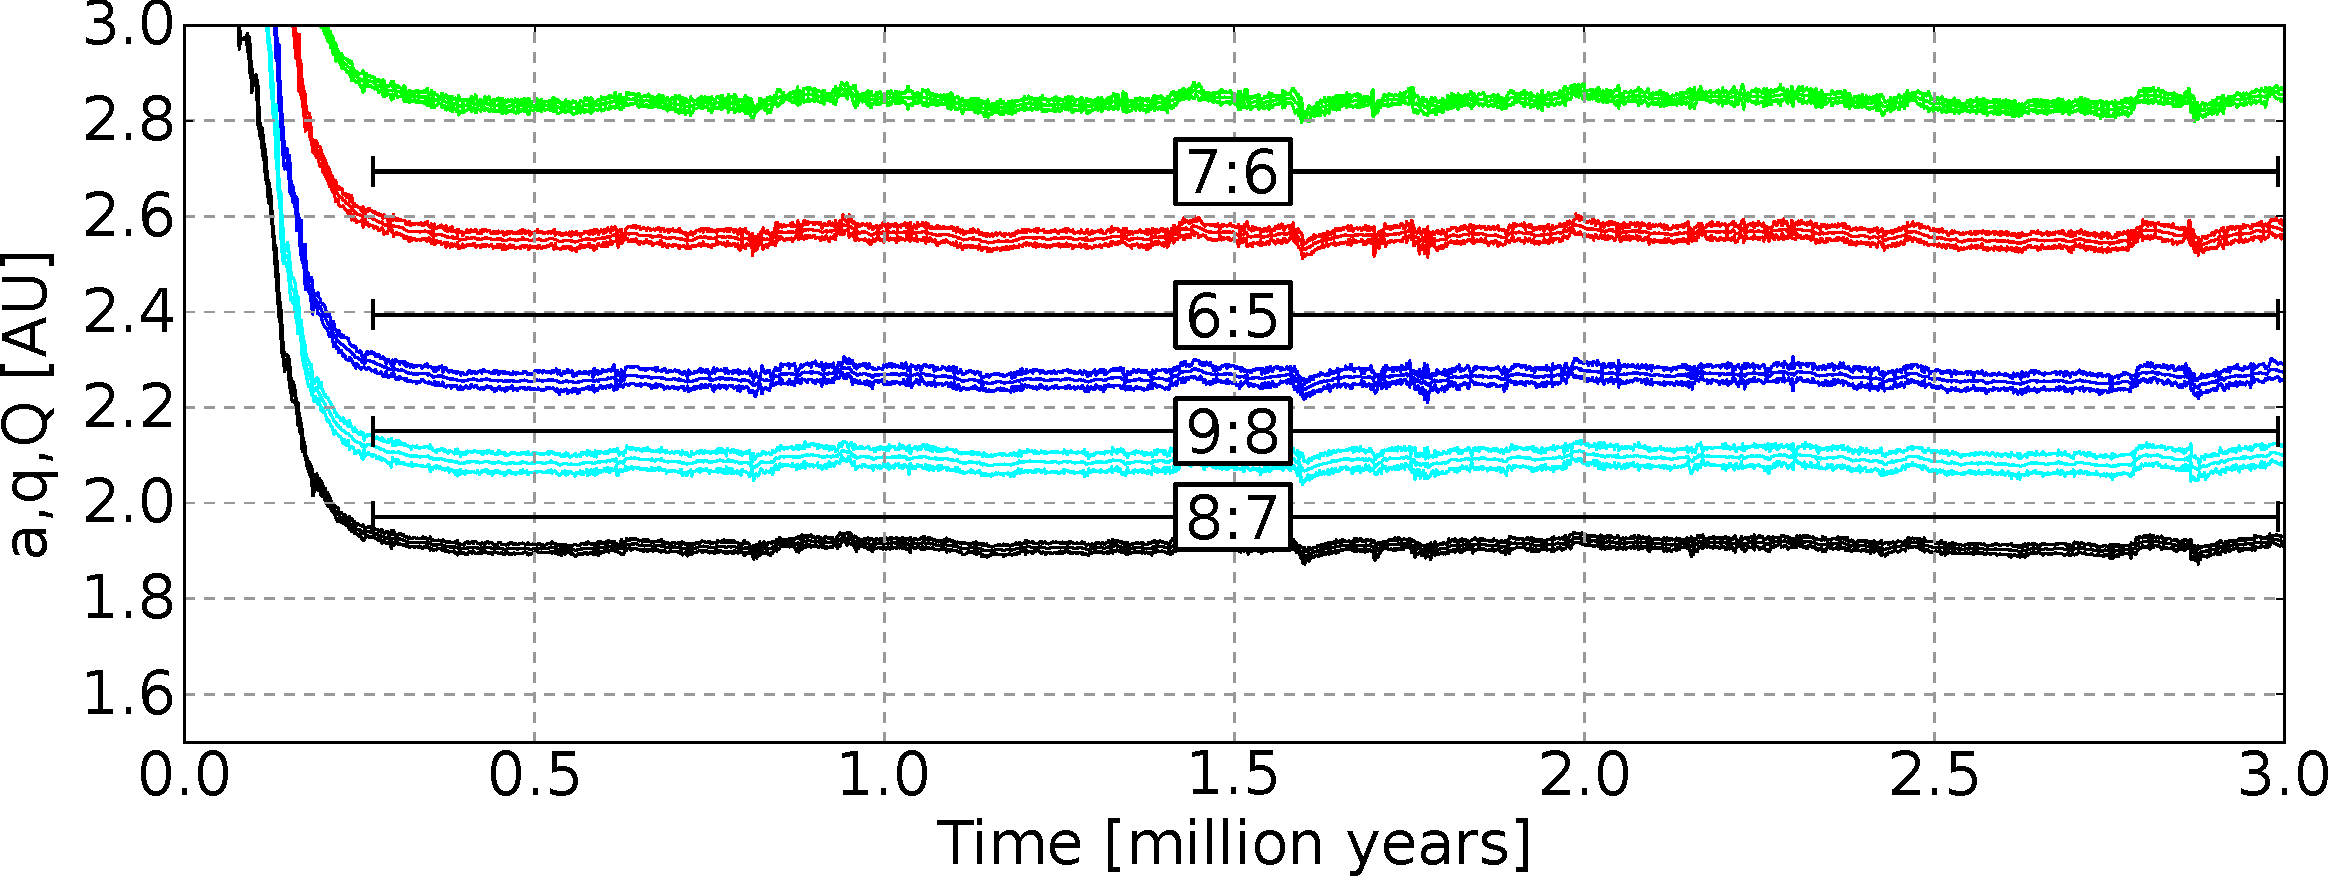
\includegraphics[width=\linewidth]{figure/shifted/5_simu00009_stable.pdf}\\
%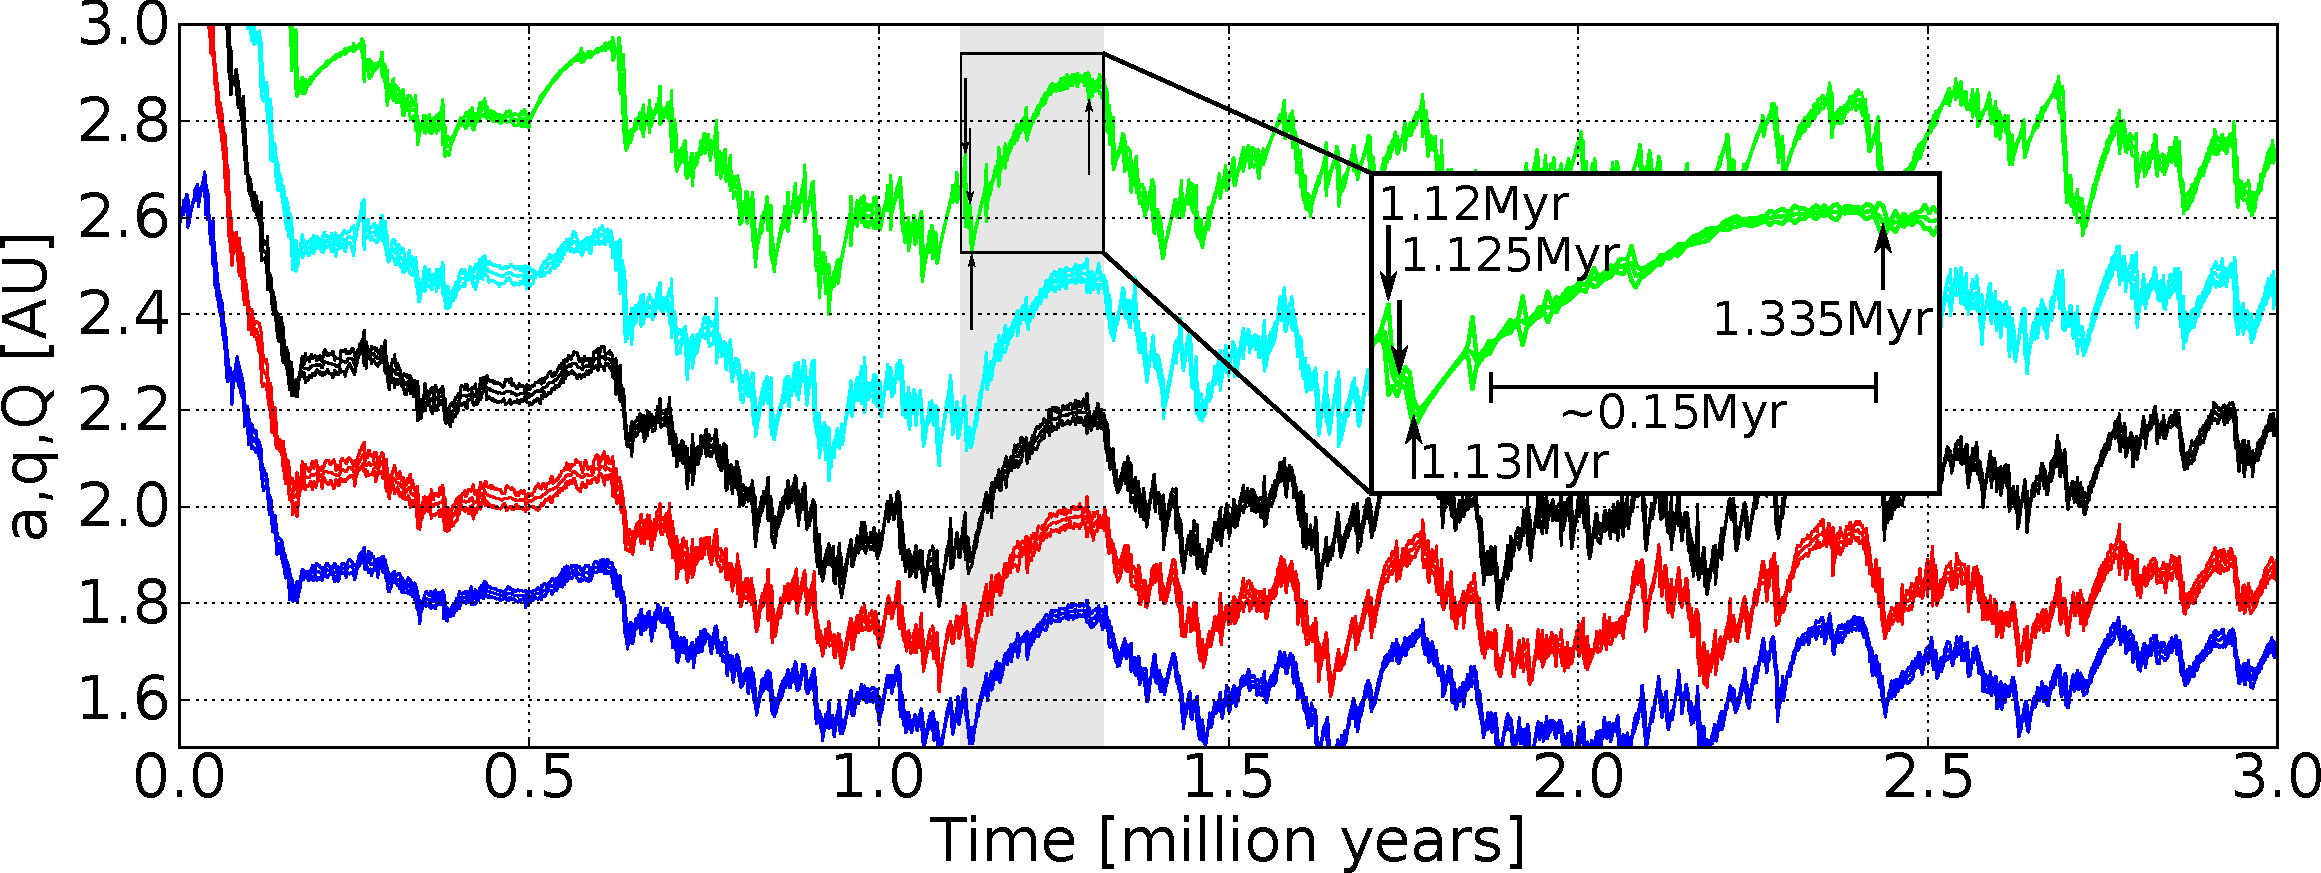
\includegraphics[width=\linewidth]{figure/shifted/5_simu00010_unstable.pdf}
%\caption{Deux exemples de simulations avec 5 planètes, une qui est relativement stable, même si de courts épisodes de pertubations des résonances ont lieu (en haut) et une qui possède un comportement chaotique soutenu (en bas).}
%\label{fig:timed-resonance-unstable}
%\end{figure}

\begin{figure}[htb]
\centering
\subfloat[Simulation relativement stable, même si de courts épisodes de pertubations des résonances ont lieu]{\label{fig:timed-resonance-stable}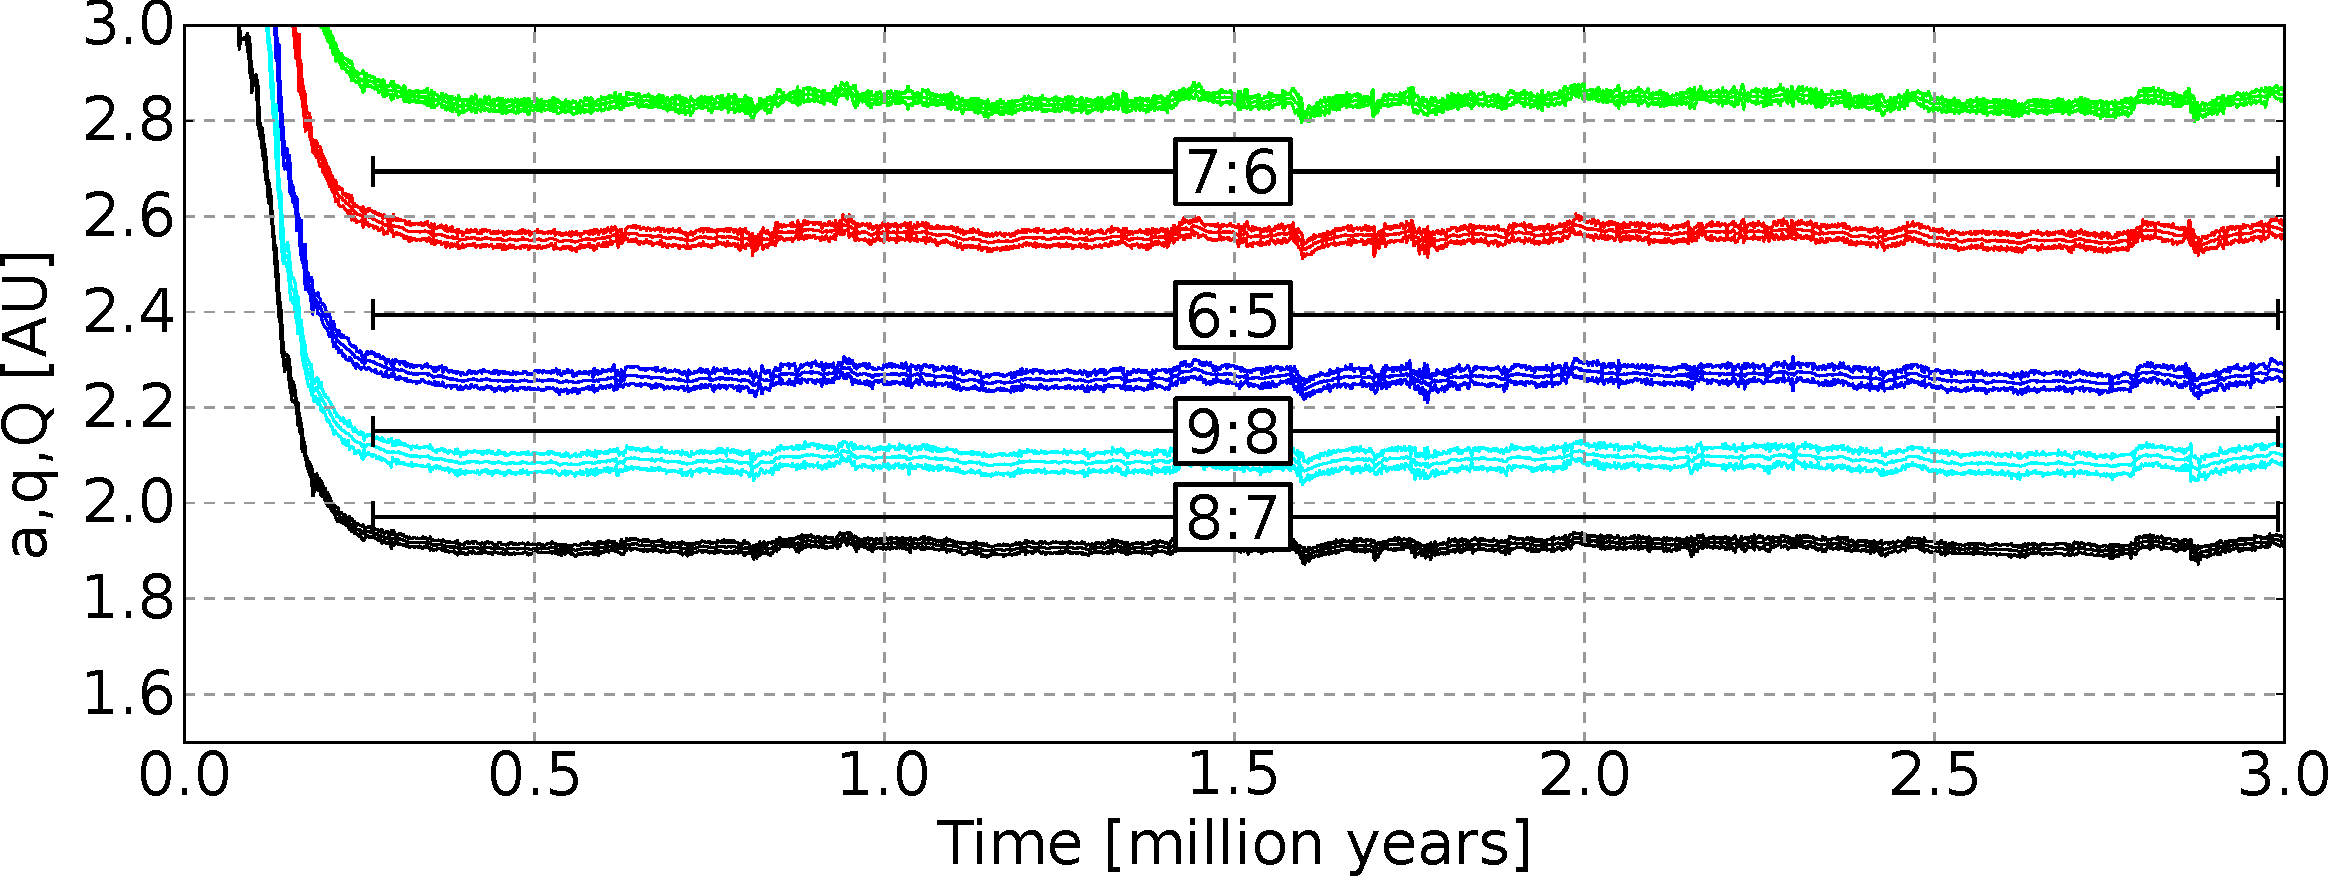
\includegraphics[width=\linewidth]{figure/shifted/5_simu00009_stable.pdf}}\\
\subfloat[Simulation qui possède un comportement chaotique soutenu]{\label{fig:timed-resonance-unstable}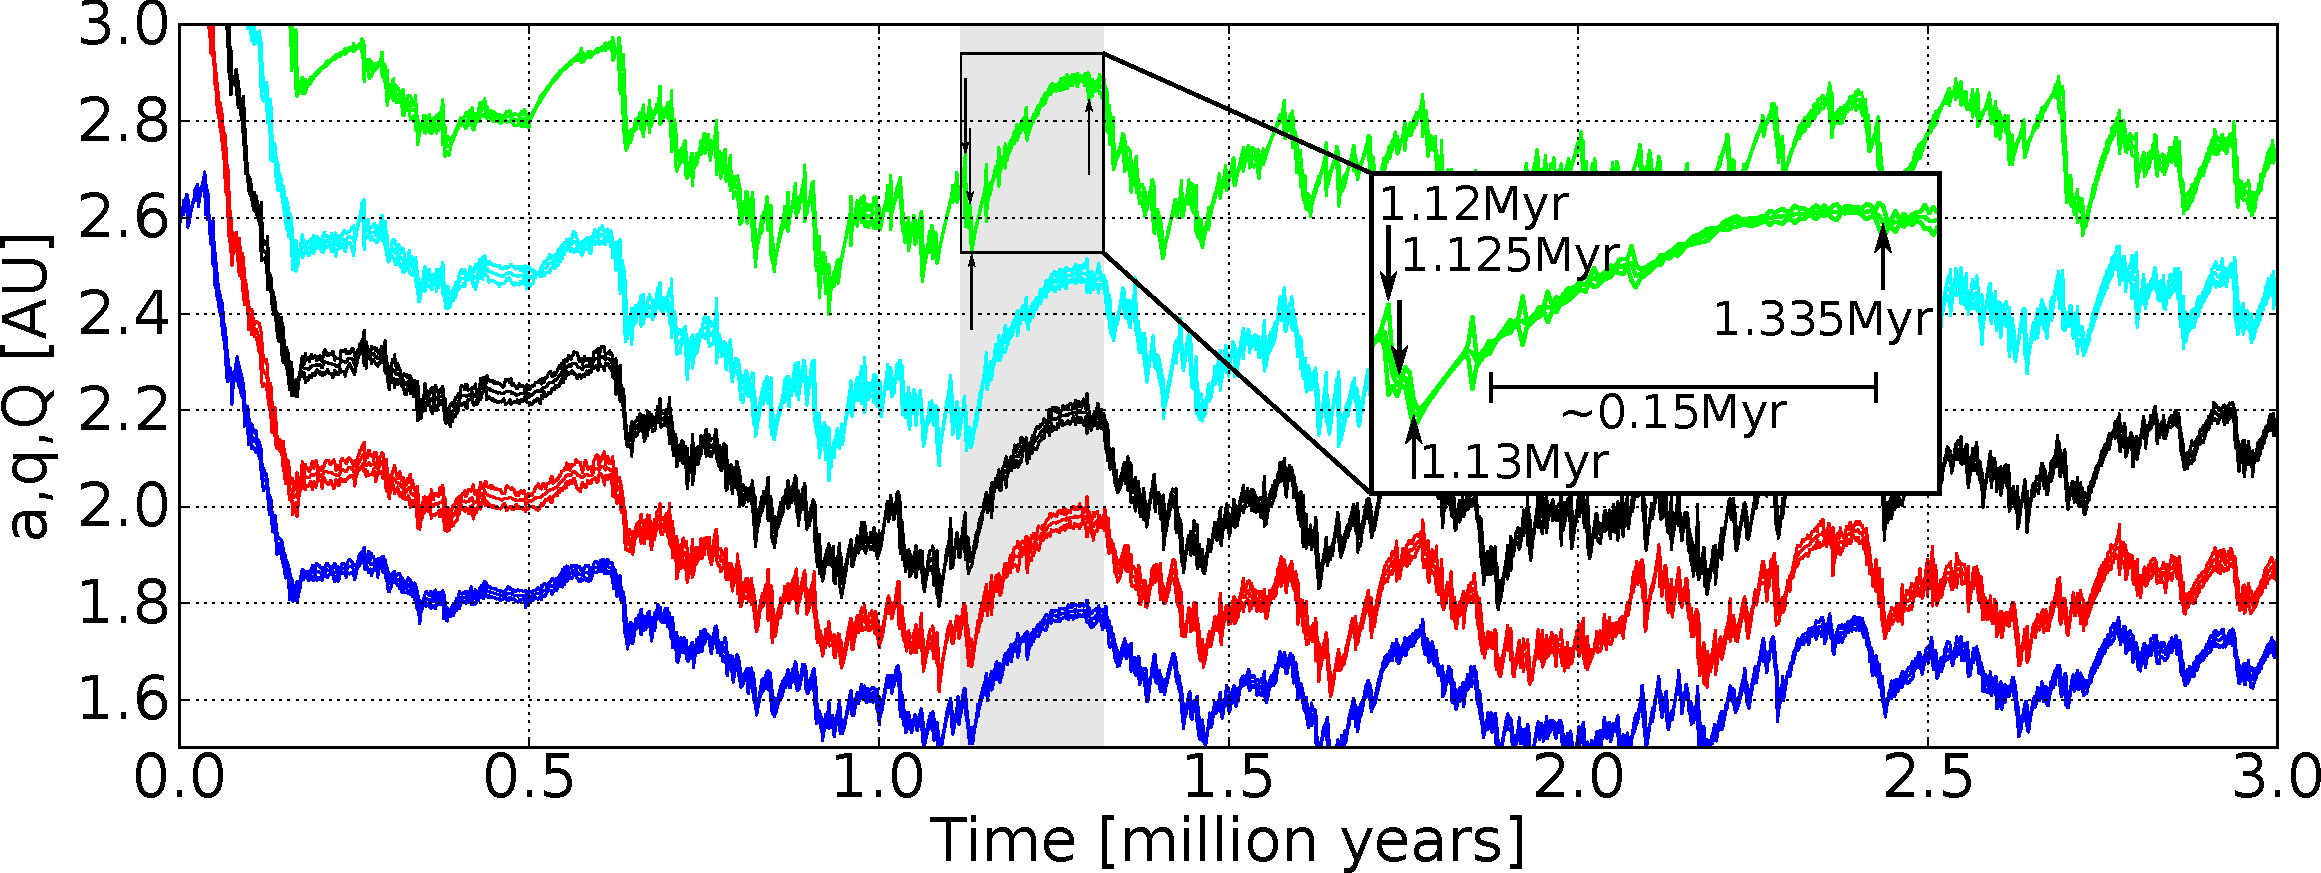
\includegraphics[width=\linewidth]{figure/shifted/5_simu00010_unstable.pdf}}
\caption{Deux exemples de simulations avec 5 planètes}\label{fig:timed-resonance-stability}
\end{figure}

Par exemple, dans la simulation \reffig{fig:timed-resonance-stable}, la chaine de  résonance subit plusieurs petites perturbations sans grandes conséquences car leur amplitude est faible devant la distance entre les planètes. Par opposition, les perturbations de la simulation  \reffig{fig:timed-resonance-unstable} sont bien plus importantes.

Considérons en particulier l'épisode chaotique entre 1.1 et 1.3 million d'années dans le cas décrit \reffig{fig:timed-resonance-unstable}. À 1.12 million d'années, les deux planètes externes sont piégées dans une résonance orbitale \MMR{4}{3}. Elles migrent alors vers l'intérieur, à cause de la soudaine excitation de leurs excentricités via la résonance. Cette perturbation se propage alors vers le système interne, et les excentricités de toutes les planètes augmentant soudainement, le système total se met peu à peu à migrer entièrement vers l'intérieur. 5000 ans plus tard, les deux planètes externes, encore les mêmes, sortent puis entrent de nouveau en résonance \MMR{4}{3}, perturbant de nouveau le système. Finalement, à 1.13 million d'années, les deux planètes externes sortent définitivement de la résonance \MMR{4}{3}. Retrouvant leur liberté de corps isolé, les deux planètes migrent vers la zone de convergence avec leurs excentricités de nouveau quasi nulle, la résonance n'étant plus là pour maintenir les 
excentricités face à l'amortissement du disque.

Sans le couple négatif des deux planètes externes, l'équilibre des couples du système global est modifié. En réaction, le système interne de trois planètes migre vers l'extérieur vers une nouvelle zone d'équilibre où le couple total exercé sur le système de trois planètes est nul. Ceci explique alors pourquoi les 5 planètes migrent brutalement vers l'extérieur. 

Cependant, les deux planètes externes entrent rapidement en résonance \MMR{5}{4}. Pendant les quelques 0.15 million d'années suivants, elles entrent périodiquement en résonance \MMR{5}{4} mais la migration vers l'extérieur continue car la plupart du temps elles ne sont pas en résonance et leur excentricité reste relativement faible. La migration globale vers l'extérieur du système s'arrête à 1.335 million d'années quand les deux planètes externes traversent la résonance \MMR{5}{4} et sont piégées dans la résonance orbitale \MMR{6}{5}. Cette configuration stabilise le système, excite les excentricités des planètes externes et entraine la migration globale du système tout entier vers l'intérieur, marquant la fin de cet épisode chaotique. 

\bigskip

Le reste de l'évolution est composé du même type de perturbations. Les perturbations proviennent des planètes qui entrent ou sortent des résonances, et qui se propagent alors au reste du système. 

Quand les planètes sortent de résonance, leur excentricité décroit rapidement, entrainant une migration vers l'extérieur. Par opposition, les planètes entrant en résonance voient leur excentricité croitre et être maintenue à un niveau constant non nul qui entraine une migration vers l'intérieur. 

Au travers de ces perturbations, des systèmes entiers subissent des migrations chaotiques relativement modestes qui illustrent la difficulté pour le système de maintenir une chaine de résonance pendant de longues périodes. 

La totalité des systèmes de 5 planètes que nous avons modélisés est restée stable, dans le sens où aucune collision n'a eu lieu. Mais l'amplitude de la migration chaotique subie par le système varie d'un système à l'autre. Les deux exemples de \reffig{fig:timed-resonance-stability} montrent les deux cas les plus extrêmes. Les simulations avec 10 planètes étaient encore plus chaotiques et des collisions ont eu lieu. 

\bigskip

Le point le plus important pour déterminer l'amplitude des oscillations chaotiques d'un système est l'ordre des résonances. Des résonances d'ordre $p$ faible (par exemple \MMR{3}{2}) maintiennent des excentricités élevés et sont moins stables car elles sont sensibles aux variations d'excentricité. Dans le même temps, les résonances d'ordre $p$ élevé (par exemple \MMR{11}{10}) maintiennent des excentricités plus faibles et sont moins sensibles aux perturbations d'excentricité.

Par exemple \reffig{fig:timed-resonance-stable}, les perturbations sont rapidement amorties tandis que dans le panneau du bas, la fréquence des perturbations est suffisamment importante pour que le système n'ait pas le temps de les amortir et ne tendent donc pas vers une configuration stable. \emph{Dans ce contexte, un système compact est donc plus stable qu'un système plus étendu, ce qui est exactement l'opposé d'une situation purement gravitationnelle} \citep{marchal1982hill}.

\subsection{Discussion}
Au travers de cette partie, nous avons montré que les planètes ne sont pas forcément piégées à la zone de convergence. Au lieu de cela, les embryons migrent rapidement vers la zone de convergence et sont piégés dans des chaînes de résonance. Ceci entraine l'augmentation brutale de leur excentricité qui reste suffisamment importante pour atténuer le couple de corotation. La zone d'équilibre de la chaîne de résonance dans le disque est déterminée par la somme des couples ressentis individuellement par les planètes (chaque terme étant la somme d'un couple de corotation atténué et d'un couple différentiel de Lindblad non atténué). Dans la pratique, cette zone de couple nul effective est déterminée principalement par la zone de convergence décalée de la planète la plus massive de la chaîne de résonance. Ce n'est pas une vraie zone de convergence car chaque planète voit une zone de convergence différente en fonction de son excentricité.

\bigskip

Le décalage vers l'intérieur existe parce que les excentricités des planètes sont maintenues par les perturbations résonantes. L'amplitude de l'excentricité d'une planète est le résultat de la compétition entre l'excitation résonante et l'amortissement de l'excentricité par le disque. Pour des excentricités suffisamment importantes, un système entier de planètes en résonance peut migrer jusqu'au bord interne.

Changer les propriétés du disque pourrait ainsi changer les valeurs typiques des excentricités en modifiant le temps caractéristique d'amortissement des excentricités. Cependant, changer les propriétés du disque a aussi des conséquences sur d'autres grandeurs influençant le système, tel que le profil de couple exercé par le disque sur les planètes. En changeant les propriétés du disque, il n'est pas évident de dire quelles seront les conséquences sur l'évolution des planètes, compte tenu du fait que les planètes pourront être dans des résonances différentes, avec des excentricités et des critères de stabilité différents. 

La zone de convergence dépend des paramètres du disque tels que la viscosité, les profils de température et de densité de surface \citep[voir par exemple][]{paardekooper2011torque}.Ici, nous avons utilisé un profil de disque issu de modèles complexes, mais qui reste malgré tout artificiel. Même si les résultats dépendent d'un modèle particulier, ils sont robustes aux variation du profil de couple en fonction de la distance orbitale, tant qu'une zone de convergence existe pour rassembler les embryons au cours de l'évolution. 

\bigskip

Dans un disque plus réaliste, on s'attend à quelques différences. En premier lieu, il pourrait exister plusieurs zones de convergence dans un même disque ayant pour origine des processus physiques différents \citep{lyra2010orbital, hasegawa2011origin}. 

Ensuite, des zones de convergences dépendantes de la masse des planètes peuvent exister dans les parties externes du disque, où ce mécanisme devrait être moins efficace compte tenu du fait que dans de telles zones de convergence, les embryons de masse différentes ne migrent pas à la même position dans le disque. Dans de telles zones, il pourrait être beaucoup plus difficile de former les chaînes de résonances essentielles pour notre mécanisme.

Troisièmement, alors que le disque se dissipe, le profil de couple et la position des zones de convergences sont aussi altérées \citep{lyra2010orbital, horn2012orbital}. 

Enfin, la turbulence est censée être commune dans les disques protoplanétaires \citep{armitage2011dynamics}. Même si la turbulence n'affecte pas l'évolution à long terme d'une planète isolée dans un disque radiatif \citep{pierens2012protoplanetary}, on s'attend à ce qu'elle modifie la capture en résonance et l'évolution des excentricités \citep[voir][]{pierens2011dynamics}.

\section{Formation des super-Terres chaudes}\label{sec:4.2}
Les détections d'exoplanètes par vitesse radiale et transit montrent que $30$ à $50\%$ des étoiles de la séquence principale possèdent au moins une planète de moins de $10\mearth$ sur des orbites comprises entre $85$ et $100$ jours \citep{mayor2011road, howard2010occurrence, howard2012occurrence, fressin2013false}. De plus, les super-Terres ($1-10\mearth$) chaudes sont préférentiellement détectées dans des systèmes multiples \citep{udry2007statistical, lissauer2011architecture}. Pourtant, même si ces systèmes peuvent nous sembler bien plus compacts que le système solaire au premier abord, d'un point de vue gravitationnel, ils possèdent à peu près le même espacement en terme de rapport de période et de rayon de Hill mutuel \citep{fang2013planetary}.


\reffig{fig:multiplanet_stats} montre les propriétés statistiques des planètes détectées dans des systèmes multiples, incluant les candidats Kepler.%TODO raconter plus de choses sur les stats?

\begin{figure}[htb]
\centering
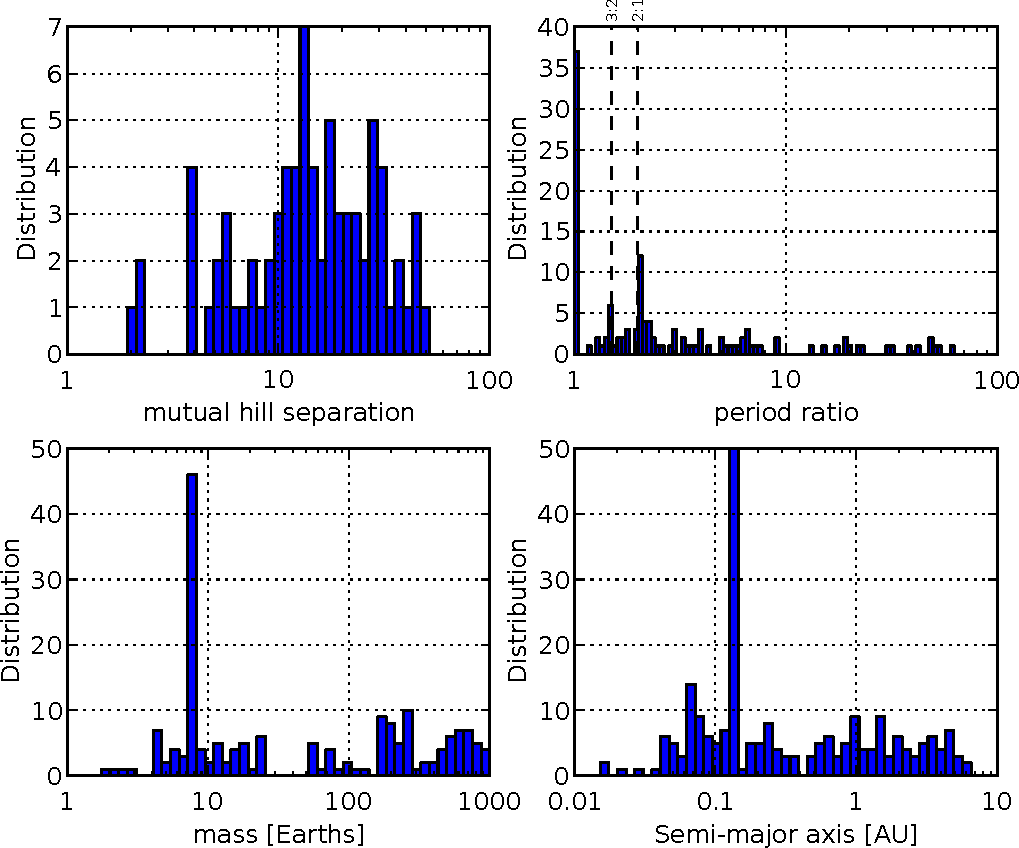
\includegraphics[width=0.8\linewidth]{figure/multiplanet_systems_stats.pdf}
\caption{Propriétés des exoplanètes détectées dans des systèmes multiples ($N\geqslant 2$). Données (01/01/2013) : \url{http://exoplanets.org/}}\label{fig:multiplanet_stats}
\end{figure}

\bigskip

Plusieurs mécanismes de formations tentent d'expliquer la présence de super Terres, ces planètes ayant une masse de $1$ à $10\mearth$, tout en étant compatible avec les contraintes observationnelles. Deux modèles principaux peuvent à ce jour expliquer la formation de ces planètes. 

Le premier modèle, la \og formation \textit{in-situ}\fg \citep{chiang2013minimum} n'est possible que si le disque est suffisamment massif localement pour permettre la formation de planète de plusieurs masses terrestres. La formation est alors semblable à celle des planètes telluriques dans le système solaire \citep{wetherill1990formation, kenyon2006terrestrial}.

Le deuxième modèle implique la migration de type 1 \citep{terquem2007migration}. Dans ce cas là, il n'est pas nécessaire de supposer un disque extrêmement massif afin de former plusieurs super terres. 

Les deux modèles permettent d'expliquer l'espacement observé. Le modèle impliquant la migration de type 1 prédit aussi que les systèmes multiples vont être proches de résonances de moyen mouvement. On peut en effet observer des pics sur \reffig{fig:multiplanet_stats} autour des résonances \MMR{3}{2} et \MMR{2}{1}. Dans le cas de la formation \textit{in-situ}, on s'attend à des planètes assez pauvres en eau, alors qu'en impliquant la migration, la variété de composition des planètes ainsi formées est beaucoup plus grande \citep{raymond2008observable}.

Il existe de plus d'autres modèles, impliquant des résonances séculaires avec des planètes géantes plus loin dans le système, la photo-évaporation de super Neptunes, circularisation des planètes excentriques. Ces modèles sont présentés et comparés dans \cite{raymond2008observable} et ne sont pas discutés ici. 

%TODO 
%Observations : contraintes en fonction de la masse des planètes, séparation (en delta, et en p2/p1)
%
%autres modèles : 
%-in-situ (murray & hansens, ou chiang & laughlin, raymond 2008) il y a un résumé de tous les modèles dans raymond 2008
%-type I migraiton (terquem & papaloizou)
%
%_______
%environ une ou deux page pour cette intro

%TODO parler des raisons de la migration vers l'intérieur (intérieur car faible masse, ou intérieur car corotation damping). 
%TODO Parler aussi de ce qui arrête les planètes au bord interne. Faire des tests pour ça.

\subsection{Modèle}
Nous utilisons les formules de \cite{paardekooper2011torque} afin de modéliser la migration de type I. Cette migration est implémentée de manière cohérente dans tout le disque. Le bord interne est simplement modélisé par une diminution brutale de la densité de surface, mais le couple induit est lui toujours calculé selon les mêmes formules. 

L'amortissement de l'excentricité et de l'inclinaison est lui issu des formules de \cite{cresswell2008three}. 

Plus de détails sur le modèle utilisé sont disponibles \refsec{sec:code_n-corps}.

Le disque utilisé possède les paramètres suivants\footnote{voir \refsec{sec:variables} pour la signification des symboles usuels} : 
\begin{align*}
b/h &= 0.4\\
\gamma &= 7/5\\
\mu &= 2.35\\
\alpha &= 5\cdot 10^{-3}\\
T_\star &= 5700\unit{K}\\
R_\star &= 4.65\cdot 10^{-3}\unit{AU}\\
\text{Disk Albedo} &= 0.5\\
\Sigma(R) &= 300 \cdot R^{-1/2}\unit{g/cm^2}
\end{align*}

La migration d'une planète dans ce disque est représentée \reffig{fig:migration_map_HSE}. Ce graphique permet de visualiser les zones de stabilités et l'évolution future d'une planète dans un disque en fonction de sa masse et de sa position initiale. Quand le couple est positif, la planète migre vers l'extérieur (vers la droite du graphique). Quand le couple est négatif, la planète migre vers l'intérieur (vers la gauche du graphique). Au cours de sa migration, si la planète rencontre une ligne noire, cela signifie qu'elle s'arrête là, car le couple de migration est nul. Cette lecture n'est possible que pour des planètes isolées dont l'excentricité est faible. En effet, les perturbations induites par d'autres planètes peuvent modifier l'état final prédit par un tel diagramme, de même que l'amortissement du couple de corotation par l'excentricité d'une planète, qui va lui totalement changer le couple de migration ressenti par la planète. 

\begin{figure}[htb]
\centering
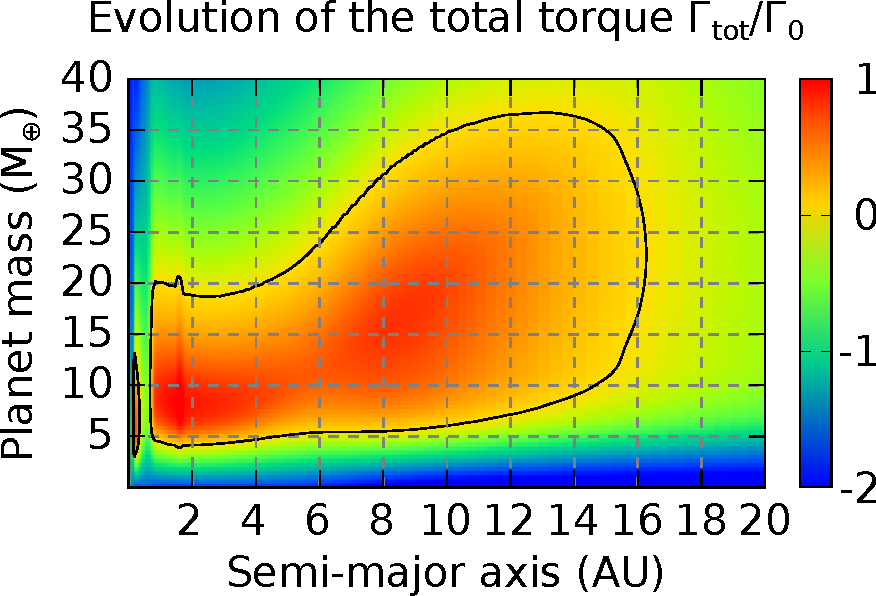
\includegraphics[width=0.65\linewidth]{figure/HSE/HSE_migration_map.pdf}
\caption{Cette carte représente l'effet du disque sur une planète en fonction de sa position en abscisse et de sa masse en ordonnée. La ligne noire représente la zone de couple nul, c'est à dire une zone où la migration de la planète s'arrête. Cette carte n'est valable que pour des planètes sur des orbites circulaires ($e\ll1$), c'est à dire quand l'amortissement du couple de corotation par l'excentricité est négligeable.}\label{fig:migration_map_HSE}
\end{figure}

Un zoom sur le bord interne du disque \reffig{fig:HSE_mig_zoom-in} montre la zone de couple positif juste avant le bord interne, dû à la décroissance rapide de la densité de surface et l'important couple de corotation qu'il engendre.

\begin{figure}[htb]
\centering
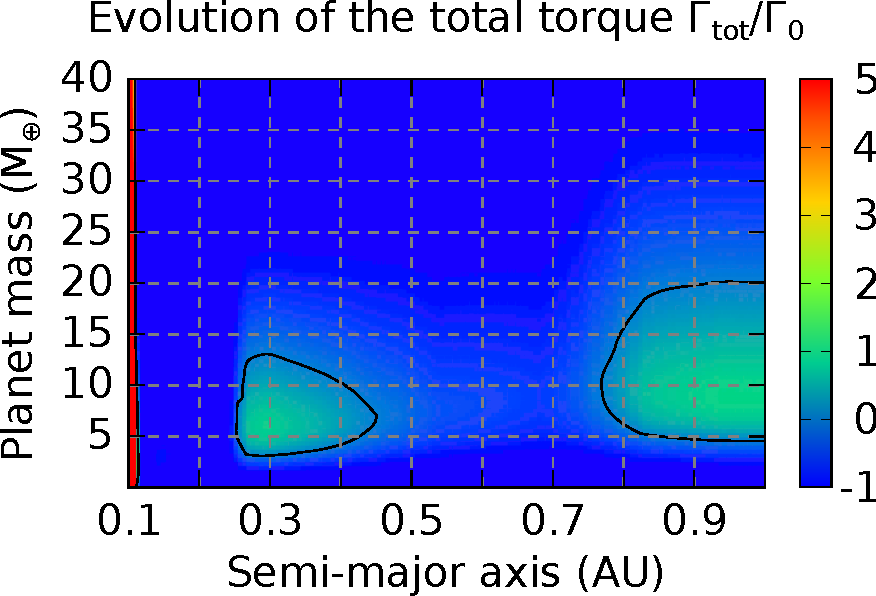
\includegraphics[width=0.65\linewidth]{figure/HSE/HSE_zoom-in.pdf}
\caption{Cette carte représente la migration d'une planète près du bord interne en fonction de sa position en abscisse et de sa masse en ordonnée. La ligne noire représente la zone de couple nul, c'est à dire une zone où la migration de la planète s'arrête. Cette carte n'est valable que pour des planètes sur des orbites circulaires ($e\ll1$), c'est à dire quand l'amortissement du couple de corotation par l'excentricité est négligeable.}\label{fig:HSE_mig_zoom-in}
\end{figure}

\subsection{Conditions initiales}
Initialement dans le système, on génère des embryons dont la masse varie de $0.1$ à $2\mearth$, pour une masse totale allant de $30$ à $100\mearth$. Des masses aléatoires différentes d'un embryon à l'autre permettent d'éviter les biais dûs aux masses égales. En effet, deux embryons de même masse migrent à la même vitesse, ce qui n'a aucune raison physique de se produire systématiquement dans un disque. Deux planètes migrant à la même vitesse ne peuvent pas entrer en collision, ou se placer en résonance, deux évènements cruciaux pour notre mécanisme de formation. 

De plus, quand deux corps sont en résonance, il y a un effet du rapport de masse sur les niveaux réciproques d'excentricité. Des masses égales maximisent les perturbations gravitationnelle de deux corps en résonance \refsec{sec:mass-ratio-effect}. Quand ce n'est pas le cas, le plus gros corps est celui qui a l'excentricité la plus faible, mais c'est aussi celui qui impose la stabilisation du système de deux corps là où lui ressent le couple du disque le plus faible.
%TODO parler du fait qu'il ne faut pas prendre des masses fixes, expliquer pourquoi. Montrer des statistiques de simulations. 

\subsection{Systèmes possibles}
En dessous d'une certaine masse limite qui dépend des paramètres du disque mais qui se situe généralement entre $2$ et $10\mearth$, les planètes migrent toutes vers l'intérieur, quelle que soit leur position initiale dans le disque. Pour le disque considéré ici \reffig{fig:migration_map_HSE}, cette limite se situe environ à $4\mearth$.

L'évolution peut suivre deux cas de figures différents, mais non exclusifs.

Dans un premier cas, les embryons migrent vers l'intérieur et il n'y a pas suffisamment de collisions durant leur migration pour qu'ils puissent migrer vers l'extérieur à un quelconque moment. On se trouve alors dans le cas d'une formation au bord interne décrite \refsec{sec:inner_edge_formation}. 

Dans un deuxième cas, une ou plusieurs planètes grossissent suffisamment par collision pour ressentir un couple positif vers l'extérieur. Plusieurs sous-cas de figures sont alors possibles, décrits \refsec{sec:outward-case}.

\subsubsection{Formation au bord interne : systèmes compacts}\label{sec:inner_edge_formation}
Des embryons migrent vers l'intérieur, de manière isolée ou par vague de sous-systèmes en résonance.

En raison de la diminution rapide de la densité de surface près du bord interne, la planète ressent un fort couple positif principalement dû au couple de corotation \reffig{fig:HSE_mig_zoom-in}. 

Un système de planètes en résonance se forme alors, les planètes internes migrant vers l'extérieur, les planètes externes migrant elles vers l'intérieur. Ce système en résonance va naturellement chercher à s'équilibrer. Cet équilibre est dicté par le fait que chaque planète ressent un couple non nul, elle possède aussi une excentricité à cause des autres corps en résonance, et ce système compact est continuellement soumis à des perturbations d'autant plus importantes que le nombre de corps en résonance est grand. 

Des collisions et réarrangements ont alors lieu, diminuant ainsi le nombre de corps et augmentant la stabilité du système global. 

\bigskip

Certaines planètes peuvent entrer dans la cavité interne du disque, poussées par le système non encore stabilisé. Elles ne perçoivent alors plus aucun effet du disque, que ce soit la migration ou l'amortissement de l'excentricité et de l'inclinaison. Dans ce cas de figure, elles peuvent ne plus être en résonance avec le reste du système. 

Même si durant l'évolution, il est possible que la planète la plus interne sorte du disque, entre en collision avec l'étoile centrale, ou soit ejectée, il est très facile de maintenir un système compact au bord interne en raison du fort couple positif qui va s'exercer sur le planète la plus interne du système alors que ce dernier cherche à migrer vers l'intérieur.

\subsubsection{Migration vers l'extérieur : candidats de planètes géantes}\label{sec:outward-case}
Lors de la migration vers l'intérieur de tous les embryons, il est possible pour une planète de grossir suffisamment vite pour ressentir un couple positif. Ce couple positif est censé entrainer une migration vers l'extérieur de la planète, ce serait systématiquement le cas si cette dernière était isolée. Mais dans son voisinage se trouvent d'autres planètes qui elles migrent vers l'intérieur. Très rapidement la planète va entrer en résonance avec un embryon planétaire qui migre vers l'intérieur.

L'effet décrit \refsec{sec:shifted_CZ} s'applique alors. La migration différentielle et le rapport de masse ont ici une importance capitale. Si la différence de vitesse est trop grande, alors les deux planètes ne peuvent pas former un système en résonance. La résonance est rapidement cassée et les deux corps continuent leur migration. Ceci est d'autant plus vrai si le rapport de masse est important, car la brève augmentation d'excentricité qui a lieu lors d'une capture en résonance n'aura que peu d'effet sur la plus grosse planète. Cette dernière sera très peu sensible aux perturbations gravitationnelle de son compagnon résonant et continuera sa migration vers l'extérieur sans quasiment ralentir. 

\begin{figure}[htb]
\centering
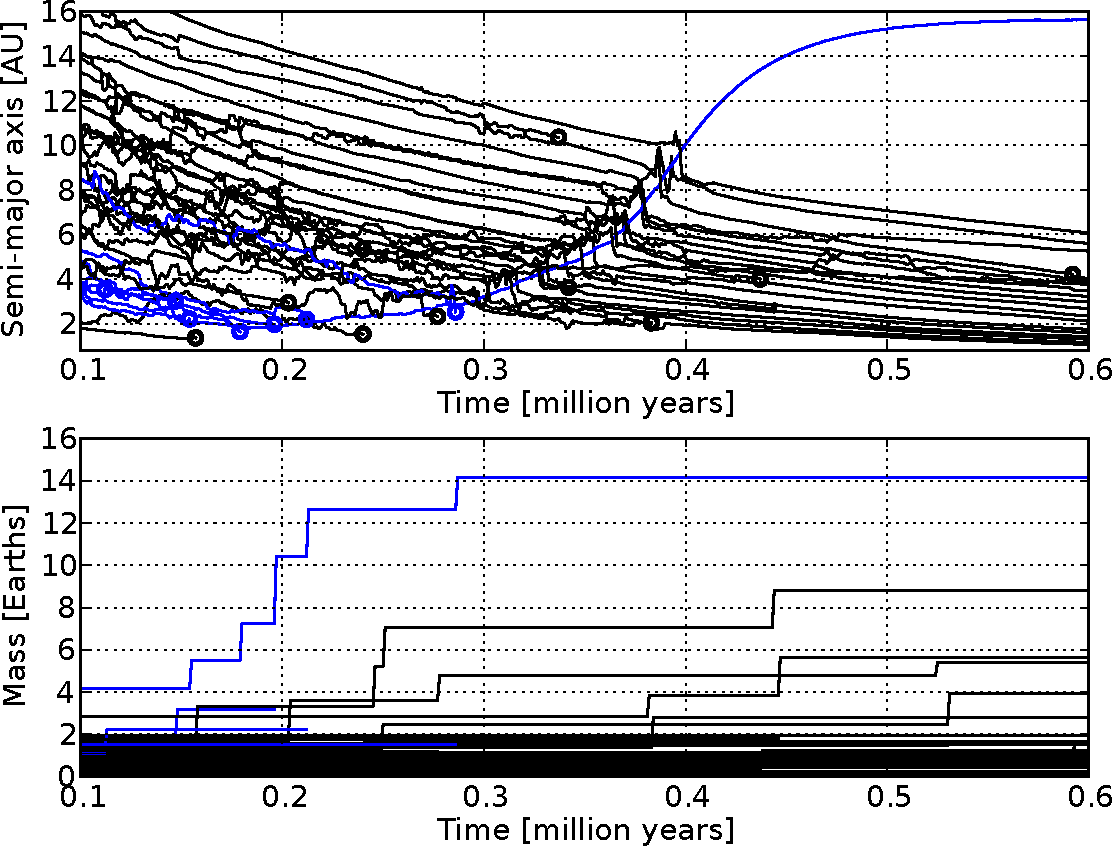
\includegraphics[width=0.65\linewidth]{figure/HSE/single_outward.pdf}
\caption{Formation d'un cœur de planète géante. La planète dont l'évolution est notée en bleu devient massive suffisamment vite pour pouvoir migrer vers l'extérieur. Les cercles représentent des collisions. Les autres courbes bleu qui disparaissent sont des embryons qui rentrent en collision avec la planète considérée et fusionnent avec elle. }\label{fig:single_outward}%/sse/cossou/HSE/disk_param/300_05/simu00010
\end{figure}

\reffig{fig:single_outward} illustre ce scénario. Cette dernière atteint par collisions la masse de $6\mearth$ au bout de $300 000\unit{ans}$ alors qu'elle se trouve à $1.2\unit{AU}$ ce qui est suffisant pour qu'elle puisse migrer vers l'extérieur. Cependant, les perturbations gravitationnelles des autres corps qui eux migrent vers l'intérieur l'empêchent de se comporter comme une planète isolée. Dans les quelques dizaines de milliers d'années suivants, 3 nouvelles collisions ont lieu. La planète fait maintenant $13\mearth$. La différence de masse avec ses voisins immédiats lui permet de migrer vers l'extérieur malgré les perturbations résonantes qui augmentent son excentricité. Comme détaillé \refsec{sec:mass-ratio-effect}, plus le rapport de masse est important, et plus la migration est dominée par la planète massive. Dans un système résonant avec rapport de masse élevé, la petite planète a une excentricité importante, son couple de corotation est fortement atténué, ce qui n'est pas le cas de la planète massive. Cette dernière migre comme si elle n'était pas en résonance, et à partir de là, soit elle emporte le système avec elle, soit, comme dans le cas présent, la résonance fini par se briser et les deux planètes continuent leur migration séparément.

Dans la suite de la simulation, la planète est trop massive pour être arrêtée. La planète massive migrant vers l'extérieur, elle capture en résonance un embryon de faible masse. Les deux planètes migrent alors vers l'extérieur, emportées par la migration de la planète la plus massive. Pourtant le système n'est pas stable. Les perturbations finissent par briser le système de deux planètes qui a alors deux possibilités. Soit une collision survient, augmentant sa masse, soit la brève rencontre se termine par un échange d'orbite. Dans cet exemple, les deux planètes continuent leur migration séparément.

À la fin de la simulation, la planète de $17.4\mearth$ est à sa zone de couple nul, à $15.7\unit{AU}$. 

\bigskip

Il est aussi possible pour la planète migrant vers l'extérieur de capturer en résonance une planète dans une configuration stable, comme le montre \reffig{fig:2-body_outward}.
\begin{figure}[htb]
\centering
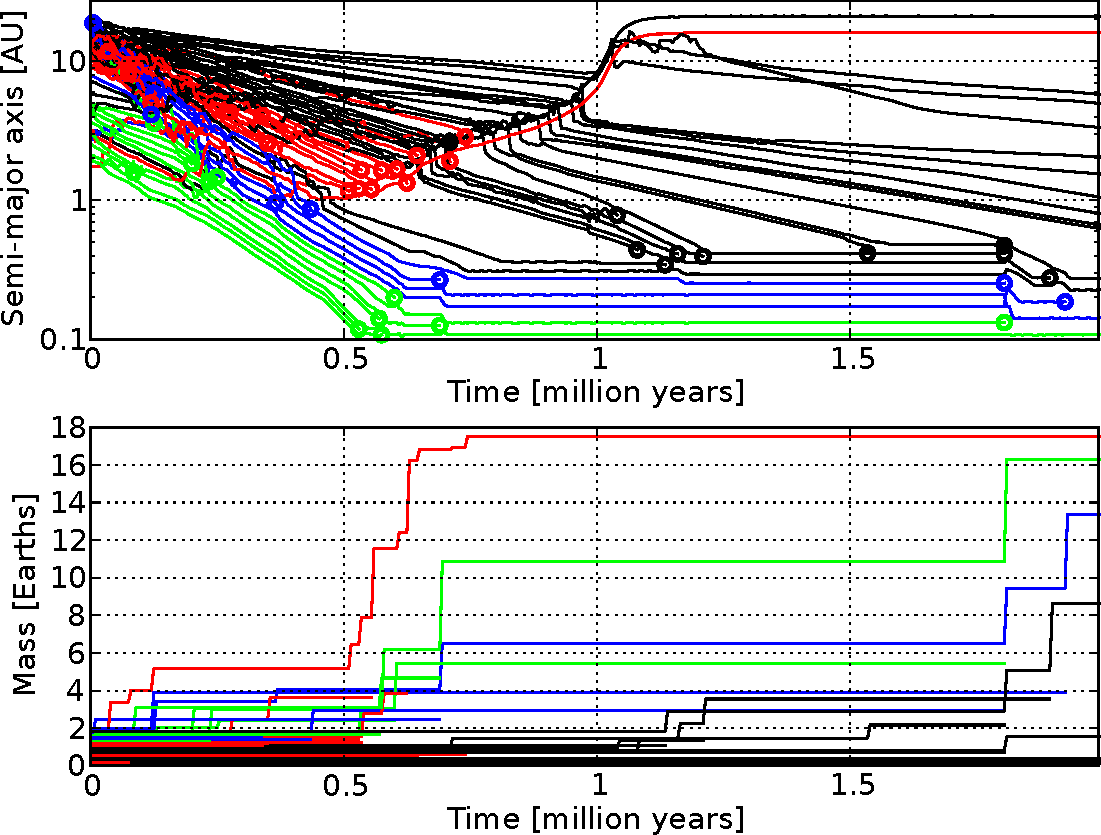
\includegraphics[width=0.65\linewidth]{figure/HSE/2-body_outward.pdf}
\caption{Formation d'un cœur de planète géante (en rouge) qui capture en résonance une planète de faible masse migrant très lentement vers l'intérieur.}\label{fig:2-body_outward}%/sse/cossou/HSE/disk_param/300_05/simu00038
\end{figure}

Dans cette même simulation, deux autres planètes massives sont formées (en vert et bleu) au bord interne, mais elles n'étaient pas massives suffisamment tôt pour migrer vers l'intérieur. Ainsi le même mécanisme, par un simple effet de timing, permet de créer soit des systèmes compacts de super terres chaudes, soit des embryons de planète géante qui pourront accréter du gaz dans les parties externes du disques, au delà de la ligne des glaces.

\bigskip

On a enfin un troisième et dernier cas où une planète grossit suffisamment rapidement pour migrer vers l'extérieur, mais est entrainée vers l'intérieur en étant capturée en résonance avec une planète de l'ordre de sa propre masse ce qui inverse son sens de migration. 

%TODO regarder la simulation %/sse/cossou/HSE/disk_param/300_05/simu00001/hires pour celà

%TODO chercher un cas où j'ai un système résonant à l'extérieur

%TODO chercher un cas où j'ai une planète qui grossi rapidement, qui veut migrer vers l'extérieur mais qui est emportéer à l'intérieur.

\subsection{Discussion}
Quand les embryons sont plus petits qu'une certaine masse critique dépendant des propriétés du disque, la migration est systématiquement vers l'intérieur. Un système compact de planètes qui grossissent par collisions se forme alors au bord interne qui retient ce système par le fort couple de corotation positif qui s'exerce juste avant le bord interne en raison de la forte décroissante de la densité de surface \citep{masset2006disk}.
%TODO le fait que le couple de lindblad est alors principalement égale au couple externe très fortement négatif ne suffit pas à contrebalancer le couple de corotation très positif. 

Pendant la migration vers l'intérieur, si un embryon grossit suffisamment vite, il peut commencer à migrer vers l'intérieur. Durant cette migration, des résonances vont se former avec les corps qui migrent pour la plupart vers l'intérieur. Par excitation résonante, la migration vers l'extérieur peut être ralentie voire stoppée, et les planètes peuvent de nouveau migrer vers l'intérieur. 

Pourtant, dans certains cas, une planète suffisamment massive peut migrer vers l'intérieur, emprisonnant des corps plus petits dans des résonances orbitales, avant de se placer à une zone de couple nul dans les parties externes du disque (dans celui présenté ici, vers $15\unit{UA}$.

\bigskip

Ce mécanisme peut alors former conjointement des systèmes compacts de super terres, proches du bord interne, ou des cœurs de planètes géantes dans les parties externes, avec possiblement des planètes beaucoup plus petites en résonance. 

La seule différence entre le cas système compact et le cas planète géante est le timing. 

En effet, il y a deux points importants. D'une part les embryons de faibles masses migrent vers l'intérieur quelle que soit leur position initiale. De plus, les embryons en dessous d'une certaine distance migrent tous vers l'intérieur quelle que soit leur masse. Les planètes qui ne répondent pas à ces critères migreront inexorablement vers le bord interne. 

Il faut donc dans le cas présent qu'un embryon atteigne la masse critique de $5\mearth$ au delà de $1\unit{UA}$ pour pouvoir migrer vers l'extérieur et devenir un cœur de planète géante.

\bigskip

Quand nous parlons ici de système compact, il faut garder à l'esprit que le disque est toujours présent. Nous ne faisons pas évoluer le disque au cours du temps, la dissipation aura donc certainement un effet. Les résonances, présentes systématiquement au bord interne à cause de la migration, auront des chances de disparaître si des déstabilisations surviennent pendant la dissipation. En effet, le système n'est stable qu'à cause de la dissipation induite par le disque de gaz. Pourtant, il est difficile de conclure car la manière dont le disque est dissipé aura une incidence sur la configuration finale du système. 

Ensuite, nous n'avons pas tenu compte de l'accrétion de gaz sur les super terres. D'un coté des planètes de plusieurs masses terrestres vont pouvoir accréter du gaz, mais la proximité de ces planètes à leur étoile centrale pourra avoir une effet dissipatif sur leur atmosphère. 

Ensuite, \cite{terquem2007migration} ont montré que la formation de systèmes compacts est possible. Ici, le modèle que nous avons repris est très similaire à leur modèle, à ceci près que nous avons modélisé la migration de manière consistante avec le disque (avec possibilité de couple positif et négatif en fonction de la masse et de la position de la planète). 

Ce que notre modèle montre en plus du modèle de \cite{terquem2007migration}, c'est que même avec migration vers l'extérieur, des systèmes compacts peuvent se former au bord interne, avec des propriétés très similaires aux propriétés des systèmes observés. Mais de plus, dans le même modèle, la formation de cœurs de planètes géantes dans les parties externes est possible. 

\section{Effets des paramètres du disque}
%TODO see kretke2012importance
%TODO regarder le papier de Bitsch 2013 et celui de 2012 où il regarde l'influence de l'indice adiabatique

Jusqu'à présent, je me suis concentré sur des cas particuliers. Dans le cas de la formation de super Terres, je n'ai montré qu'un seul disque \refsec{sec:4.2}. Dans le cas du décalage de la zone de convergence, j'ai montré un disque artificiel modélisant une zone de convergence \refsec{sec:shifted_CZ}. À chaque fois je me suis concentré sur un type particulier d'effet qui bien que présent dans plusieurs disques, n'était mis en valeur que dans un seul disque concrêt. 

Ici je vais présenter les effets de divers paramètres du disque sur la migration. 

Le nombre de paramètres pour lesquels un effet est extractible est assez restreint, pour plusieurs raisons. La première raison est que la modélisation de la migration dans un disque où les paramètres ont au mieux une variation radiale, au pire sont constants, ne reflètent évidemment pas la réalité. D'importantes incertitudes sont présentes, à la fois au niveau des modèles, des approximations mises en jeu, ou des mesures observationnelles. 

\cite{kretke2012importance} ont déjà étudié l'influence des paramètres du disque sur la migration. Cependant, s'ils ont inclus des effets fins sur le bord interne et la migration, l'opacité est par exemple une simple loi de puissance. Nous montrerons que l'opacité est un paramètre sensible du modèle et qu'il est important de la modéliser le plus finement possible. 


%TODO continuer
Je cherche ici à montrer quels paramètres ont une influence majeure sur la migration, mais il est bien évident qu'en rajoutant d'autres effets dans le disque, on modifiera encore la migration, et en particulier les cartes de migration.

%TODO 
\subsection{Viscosité du disque}
%TODO 
\subsection{Profil de densité de surface}
%TODO 
\subsection{Profil de température}
%TODO 
\subsection{Masse du disque}
%TODO 
\subsection{Table d'opacité}
%TODO 
\subsection{Longueur de lissage}
%TODO parler du travail d'audrey, essayer de la citer. Présenter le fait qu'on ne sait pas quelles valeurs donner à ce paramètre, et montrer les implications sur la migration. 

%TODO voir pierens et huré où ils prennent un cas de disque 2D avec un b/h et comparer avec un disque 3D pour trouver le bon b/h
%TODO voir aussi muller & kley 2012, il devrait y avoir des informations
%TODO essayer de parler du fait qu'il y a deux longueurs de lissage, une pour le potentiel de la planète, et une pour le potentiel du disque. Le premier génère les ondes de densité, le deuxième génère le couple sur la planète



\chapter{Discussion et limite du modèle}\label{sec:discussion}
Afin de conclure ce travail, nous allons dans un premier temps récapituler les résultats principaux de cette thèse. Nous nous attarderons ensuite sur certaines limitations importantes des modèles utilisés pour ensuite parler des perspectives futures qui découlent de ce présent travail. 

\section{Résultats}
\subsection{Cartes de migration}\index{carte de migration}
Nous avons vu dans le chapitre \refsec{sec:chap3} que les paramètres du disque avaient une influence sur la carte de migration de ce dernier. 

Si l'indice de profil a une importante \refsec{sec:sigma_index}, c'est surtout la valeur de la densité elle-même qui prédomine \refsec{sec:sigma_0}. En augmentant la densité, la partie active du disque est de plus en plus étendue. Quand la densité diminue, c'est l'irradiation qui va avoir tendance à dominer de plus en plus rapidement le profil de température. D'une manière générale, un profil plus abrupt de densité de surface comprime la carte de migration dans les parties internes. Les planètes ne peuvent plus migrer aussi loin dans le disque. De même, un disque moins massif ne permet plus aux planètes de s'éloigner autant de leur étoile par migration. 

La viscosité, en influant sur le chauffage visqueux, agit de la même manière sur la carte de migration que la densité de surface \refsec{sec:nu_constant}. En augmentant densité ou viscosité, les zones de convergence ont tendance à se décaler dans les parties externes du disques et pour des masses de planète plus grandes. 

Ces grandeurs, bien que dépendant intrinsèquement du disque considéré, vont aussi varier au cours de la dissipation du disque. Comprendre l'évolution de la migration en fonction de ces paramètres nous permet donc de mieux comprendre comment va se comporter une planète au cours de la vie du disque. Au cours de la dissipation du disque, le paramètre alpha (et donc la viscosité) va, au même titre que la densité de surface, diminuer au cours du temps \citep[Fig. 16]{guilloteau2011dual}. Prise séparément, la décroissance de ces deux paramètres va dans le même sens. Au fur et à mesure que le disque disparait les zones de convergence en font autant. Soit ces dernières se décalent jusqu'à fusionner avec le bord interne du disque, soit elles s'amenuisent jusqu'à disparaitre.

Pour une planète, les zones de convergence ont tendance à disparaître d'autant plus rapidement que la planète est massive. Mais au fur et à mesure de la dissipation du disque, des planètes peu massives peuvent migrer vers l'extérieur alors qu'elles ne pouvaient pas le faire au début de la dissipation. Tard dans la vie du disque, des zones de convergence pour les planètes de faible masse, de l'ordre d'une masse terrestre pourraient jouer un rôle important dans la formation des planètes telluriques.

\subsection{Formation de super-Terres chaudes et de noyaux de planètes géantes}\index{super-Terre}\index{noyau de planète géante}
Dans le chapitre \refsec{sec:chap4}, j'ai montré qu'une même population statistique d'embryons pouvait aboutir à la formation d'un système compact de super-Terres chaudes ou à la formation d'un ou plusieurs embryons de planètes géantes. Dans le modèle, un noyau de planète géante est un embryon planétaire qui devient massif ($m>5\mearth$) suffisamment rapidement pour inverser sa migration et repartir vers l'extérieur, vers une zone de convergence située autour de $15\unit{UA}$ dans le disque présenté. Dans ce même modèle, nous obtenons des super-Terres si les embryons migrent vers l'intérieur plus rapidement qu'ils ne grossissent en masse. Ainsi, cette masse est transportée dans les régions internes où un système compact d'embryons en résonance de moyen mouvement apparaît, maintenu dans le disque grâce au fort couple de corotation qui apparaît au bord interne.

Pour un même disque de gaz, si on diminue la quantité de masse disponible pour les embryons planétaires, alors nous formons toujours des systèmes compacts de super-Terres, mais nous ne formons pas ou peu de cœurs de planètes géantes. En accord avec les observations, nous observons donc que la métallicité d'une étoile ne diminue pas la probabilité de formation d'une super-Terre \citep{howard2012occurrence}, tandis qu'elle influe grandement la formation de planètes géantes \citep{johnson2007new}. 

\bigskip

Le principal défaut de ce modèle de formation est pour l'instant son incapacité à former des noyaux de planètes géantes de manière isolée, c'est-à-dire sans la présence d'un système compact de super-Terres chaudes dans les parties internes du disque. En partant d'une population d'embryons dont les masses sont aléatoires et suivent une distribution uniforme, il est nécessaire de partir d'une masse totale d'embryons importante ($M_\text{tot}>30\mearth$) afin de former des cœurs de planètes géantes. Une fraction non-négligeable de cette masse arrive malgré tout près du bord interne, résultant en la création d'un système compact de super-Terres, avec ou sans planètes géantes. Une solution pour remédier à ce problème serait de trouver une configuration dans laquelle on peut former un cœur de planète géante avec une quantité de masse réduite. Ainsi, si un cœur de planète géante se forme, la masse restant dans le système serait insuffisante pour former un système compact au bord interne. 

\bigskip

Lors de la \gras{dissipation du disque}, en particulier dans la deuxième phase où la photo-évaporation joue un rôle majeur, le bord interne va être fortement modifié. En conséquence, la stabilité des systèmes compacts de super-Terres sera affectée. La manière dont le bord interne sera modifié avec le temps ainsi que le profil de densité de surface dans son voisinage sont des paramètres clé dont les effets restent à quantifier. 

De plus, dans notre modèle nous n'avons pas pris en compte l'\gras{accrétion de gaz}. Or une partie au moins des planètes que nous
formons ont des masses à partir desquelles l'accrétion de gaz commence. L'accrétion de gaz, en accélérant la croissance en
masse des embryons pourrait augmenter la probabilité de former des cœurs de planètes géantes dans les parties externes du
disque, ces derniers pourraient en effet accéder à la zone de migration vers l'extérieur plus facilement. Dans le même temps, la
proximité des super-Terres chaudes avec leur étoile doit aussi avoir une influence sur la survie de leur atmosphère, la photodissociation, et la température de l'atmosphère influant sur le taux d'échappement. 

La continuité de mon travail serait d'inclure la dissipation du disque, l'accrétion de gaz et la migration de Type II afin de voir d'un part si les systèmes compacts survivent à la dissipation du disque et d'autre part de quantifier la formation de planètes géantes à partir des noyaux que nous formons déjà.

\section{Limitations des modèles}
\subsection{Longueur de lissage}\index{longueur de lissage}
La migration de Type I que nous utilisons est issue des formules de \cite{paardekooper2011torque}. Même si ces formules sont utilisées ici dans un disque 1D où le profil de température, de densité de surface, et le rapport d'aspect changent en fonction de la distance, la formule originelle suppose que localement, dans une zone d'environ $\pm H$ autour de la planète, le rapport d'aspect et les indices des profils de température et densité de surface sont constants. 

Ces formules analytiques ont été calculées puis ajustées à des simulations hydrodynamiques 2D. Une comparaison indépendante des formules avec d'autres simulations hydrodynamiques 2D trouve un bon accord avec ces formules, excepté le fait que la migration est plus lente dans les simulations hydrodynamiques 2D \citep{pierens2013makingaccepted}. 

Le biais le plus important introduit par cette formule est qu'elle dépend fortement de la longueur de lissage $b/h$. Le problème est qu'il n'existe pas de valeur optimale de la longueur de lissage à la fois pour les couples de Lindblad et de corotation \citep{masset2002coorbital}. En effet, le couple de corotation provient de régions au plus proche de la planète, qui sont totalement modifiées par la taille de la zone lissée autour de la planète. La longueur de lissage optimale tend à être plus petite si on veut modéliser correctement le couple de corotation, alors qu'elle doit être légèrement supérieure si on s'intéresse au couple de Lindblad. 

Il semble impossible de modéliser une migration doublement lissée dans un code hydrodynamique 2D qui modélise le disque et la migration avec précision. Une solution approchée serait de modéliser artificiellement deux longueurs de lissage dans les codes N-corps \reffig{fig:modified_smoothing}, une pour le couple de Corotation et une pour le couple de Lindblad. Il faut toutefois vérifier que le résultat permet de contourner une limitation numérique des codes 2D en n'introduisant pas de biais ou d'erreur plus importante que le gain que l'on cherche à obtenir. Une étude des simulations 3D, où l'introduction d'une longueur de lissage n'est pas nécessaire, et des simulations N-corps semble donc nécessaire pour s'en assurer. 

\subsection{Modélisation de la densité, température et viscosité dans un disque}
La formule du couple de migration dépend des paramètres du disque et de leur évolution au sein de ce dernier. 

Notre modèle consiste en un disque avec un profil de densité de surface en loi de puissance fixe, puis nous calculons le profil de température $T$, de rapport d'aspect $h=H/R$, de diffusivité thermique $\chi$, d'opacité $\kappa$ et de profondeur optique $\tau$ en fonction du rayon. Nous avons donc un disque 1D. Nous n'avons pas de dépendance explicite en fonction de la hauteur du disque. 

La plus grande incertitude de notre modèle est l'approximation qui consiste à dire que depuis le bord interne jusqu'au bord externe, nous avons une évolution en loi de puissance de la densité de surface $\Sigma\propto R^{-d}$ dont l'indice $d$ est fixe. Quand $d>1$, pour une masse de disque constante, la masse se trouve préférentiellement au bord interne résultant en des températures $T>100 000\unit{K}$ dans certaines conditions. Dans de tels disques, la modélisation atteint ses limites.

D'autres modèles fixent au contraire le profil de température pour calculer le profil de densité de surface. Enfin, dans les simulations hydrodynamiques, une viscosité $\nu$ constante est souvent choisie afin de simplifier la modélisation. Aucune de ces approximations n'est réaliste pour des distances allant de $0.1$ à $100\unit{UA}$. 
%TODO ref !!!!!

Une étude intéressante serait de voir si un modèle simplifié 1D ne pourrait pas modéliser de manière cohérente le profil de densité de surface, de température et de viscosité. La migration est maintenant disponible pour les modèles N-corps à l'aide de formules analytiques. La modélisation des rétroactions entre densité de surface, viscosité et température peut être effectuée à l'aide d'un disque simplifié, sans dépendance ni azimutale ni verticale \citep{hellary2012global}. En effet, à l'heure actuelle, quel que soit le type de simulation considéré, l'incertitude la plus élevée réside toujours dans la valeur que l'on attribue à l'un des trois profils que l'on prend pour paramètre libre, que ce soit la température, la densité de surface ou la viscosité.

\subsection{Self-shadowing}\index{self-shadowing}
La zone morte, en modifiant les trois profils à la fois, température, densité et température, rajoute encore un degré de complexité dans le modèle.

Nous avons vu \refsec{sec:shadow} que l'ombre du disque, modélisée de façon cohérente, n'était susceptible d'avoir une influence sur la carte de migration que dans une région où l'irradiation domine le profil de température. Or typiquement, la zone d'ombre se situe justement dans les parties internes du disque, là où le chauffage visqueux domine. 

Cependant, la zone morte modifie le disque de telle sorte qu'une légère surdensité se produit au bord interne de cette dernière. De plus, dû à la soudaine chute de la viscosité, le chauffage visqueux est beaucoup moins important et la zone morte est une région où l'irradiation peut dominer, bien que nous soyons dans les parties internes du disque. 

La zone morte pourrait donc être une région privilégiée du disque où l'irradiation et le \og self-shadowing\fg ont une grande importance. C'est de plus une zone d'intérêt pour la formation planétaire par le piège à planète qu'elle peut constituer \citep{masset2006disk, hasegawa2011origin}.

Il serait intéressant d'étudier l'effet conjoint de l'ombre du disque et de la zone morte sur la carte de migration et les conséquences que cela a sur la migration et formation planétaire. En effet, il semble que les deux effets résultent en la création d'une zone de convergence pour les masses très faibles \reffig{fig:dz_shadow_map} qui pourrait constituer un piège à planètes de faibles masses au cours de la vie du disque. Ce piège à planète se situe au niveau du bord interne de la zone morte, c'est-à-dire de l'ordre de $1\unit{UA}$.

\subsection{Modèle d'opacité}\index{opacité}
L'opacité joue un rôle prépondérant dans la détermination des profils radial du disque. En particulier, l'opacité a une influence majeure sur le profil de température et sur le couple de Corotation. 

En fonction du modèle d'opacité choisi, la migration d'une planète dans un disque donné peut être très différente \refsec{sec:influence_opacity_table}. 

De plus, le cadre dans lequel l'opacité est calculé est souvent négligé. Afin de calculer l'opacité, il est nécessaire de connaître les propriétés des poussières, tant leur distribution que leur composition. L'abondance de métaux est susceptible de varier d'une étoile à l'autre et avant d'avoir un effet sur la quantité de masse disponible pour la formation planétaire, ce paramètre aura un impact direct sur l'opacité dans le disque. 

Ensuite, les propriétés de la poussière sont susceptibles de varier au cours de la dissipation du disque et de la formation des planètes, même si les collisions peuvent régénérer la population de poussière.

L'abondance de planètes semble dépendre de la métallicité des étoiles autour desquelles elles orbitent \citep{fischer2005planet}. Une étude sur le sujet devrait aussi s'intéresser à l'influence de la métallicité sur l'opacité dans le disque, compte tenu du fait que ça aura une incidence sur la carte de migration qui en découle.

\subsection{Effet indirect des ondes de densité sur les autres planètes}
Le couple de migration est calculé dans des simulations où la planète est isolée. Mais comment réagi une planète aux ondes de densité d'une autre planète? 

\emph{A priori}, une planète ressent la perturbation gravitationnelle induite par l'onde de densité de Lindblad d'une autre planète. Cependant, on ne s'attend pas à ce que l'effet sur la migration soit important, notamment en raison du fait que l'onde de densité de Lindblad tourne dans le disque à la fréquence képlerienne de la planète à son origine, or cette fréquence n'a pas de lien avec la fréquence képlerienne d'une autre planète. 

Les choses pourrait être un peu différentes si par exemple les deux planètes sont en résonance de moyen mouvement. Le rapport qui existe entre leurs périodes orbitales entraine une relation similaire entre les vitesses angulaires, et donc entre l'onde de densité d'une planète et l'autre planète. À ce titre, le cas particulier des résonances co-orbitales est intéressant car les planètes ont le même demi-grand axe et la même vitesse angulaire en première approximation.

\cite{podlewska2012outward, baruteau2013disk} ont étudié l'effet indirect des ondes de densité sur les autres planètes dans le cas particulier des planètes massives. Dans un tel système, la réponse du disque n'est pas linéaire pour la deuxième planète. Aucune étude n'a été faite à ce jour sur cet effet dans le cas de deux planètes de masses comparables. 

\section{Conclusion}
J'ai cherché tout au long de ma thèse à développer un code numérique simple et modulaire avec l'idée de pouvoir tester les interactions et/ou différences entre différents modèles. L'idée était de profiter des libertés offertes par un code N-corps plus rapide pour tester des domaines de l'espace des paramètres qui ne sont pas accessibles aux codes hydrodynamiques. 

\bigskip

Dans le chapitre \refsec{sec:chap3}, j'ai étudié la migration dans les disques à l'aide de cartes de migration qui permettent de comprendre le comportement de la migration dans un disque donnée de manière assez intuitive. Dans un premier temps j'ai cherché à comprendre la forme de ces cartes de migration. Puis, j'ai cherché à comprendre l'influence des paramètres du disque sur les cartes de migration. Le code N-corps que j'ai développé m'a donné une grande liberté quant à l'espace des paramètres accessible. 

Il m'a de plus permis de tester la migration dans des conditions totalement inaccessibles aux simulations hydrodynamiques, typiquement une centaine d'embryons planétaires évoluant pendant plusieurs millions d'années. Ces simulations m'ont permis d'observer des phénomènes liés à l'interaction entre plusieurs effets isolés comme par exemple le décalage de la zone de couple nul d'un système résonant. Les simulations 3D ont montré que le couple de corotation était modifié par l'excentricité d'une planète \citep{bitsch2010orbital}. Le fait que deux planètes se placent en résonance était aussi connu. Mes simulations N-corps ont permis de montrer que lors de la formation des planètes, il était possible pour deux planètes d'être capturées en résonance, que leurs excentricités soient maintenus à un certain niveau grâce à ça, et que l'excentricité modifie le couple de corotation, et donc la position de stabilité du système résonant\citep{cossou2013convergence}. 

\bigskip

La grande diversité des disques et migrations montre que les populations synthétiques de planètes ne peuvent reproduire la population de planètes extrasolaires avec un seul type de disque. Les propriétés de l'étoile, la masse du disque, la quantité de poussière, la dissipation du disque et l'évolution subséquente de la densité de surface, l'opacité et la température doivent être prises en compte. 

Cela souligne que nous manquons cruellement de contraintes observationnelles. En particulier sur la densité de surface. Le profil de la nébuleuse solaire minimale en $R^{-\frac{3}{2}}$ est largement utilisé, mais ne correspond pas aux observations qui trouvent un profil moyen en $R^{-1}$. De plus, il est peu probable qu'une seule loi de puissance décrive correctement la totalité d'un disque. 

ALMA devrait amener des observations de très haute résolution de disques protoplanétaires, et un gain de précision sur les propriétés des disques. Ces contraintes devraient nous permettre de limiter l'espace des paramètres et de trouver quelques disques dits \og classiques\fg sur lesquels la formation planétaire pourra se concentrer. 

Il n'est pas impossible que dans le futur, certaines sous-populations particulières d'exoplanètes puissent être expliquées par un type particulier de disque. En effet, si le nombre de planètes est faible par rapport au nombre total, il est possible que ces planètes nécessitent des conditions particulières pour être formées. Dans certaines de mes simulations, j'ai pu observer la formation conjointe d'un cœur de planète géante dans les parties externes, autour de $10\unit{UA}$ et d'un système compact au bord interne ($a\sim 0.1\unit{UA}$). Aucun système extra-solaire de ce type n'a encore été trouvé. Peut-être que dans quelques années de tels systèmes seront détectés. Ce serait en tout cas un argument fort en faveur du modèle que j'ai présenté ici. 

\bigskip

Avec des observations toujours plus nombreuses, que ce soient des disques protoplanétaires ou des exoplanètes, nous avons de plus en plus de données à confronter à nos modèles de formation et d'évolution des systèmes planétaires. 

Les prochaines années seront le berceau de la révolution ALMA, en particulier dans le domaine des disques protoplanétaires. Si nous avons de plus en plus de contraintes sur l'état final des systèmes planétaires, nous avons encore beaucoup de libertés sur les conditions initiales pour les former. 

Le plus grand défi de la formation planétaire est de faire co-évoluer le disque et les planètes. En effet, ils interagissent au cours de leur vie, mais il est souvent difficile de tenir compte des deux évolutions en même temps. Pour ce faire, un seul type de simulation ne suffit pas. Afin d'étudier le problème dans toute sa complexité, il est nécessaire de calibrer, puis modéliser, depuis les plus petites échelles jusqu'aux plus larges. Les simulations N-corps s'inscrivent en bout de cette chaîne, utilisant les modèles mis au point dans des simulations complexes mais coûteuses en temps, afin d'accéder à l'immense espace des paramètres qui s'offre à nous.



\chapter*{Conclusion}
\addstarredchapter{Conclusion} % to be used in place of addcontentsline to avoid problems with minitoc
%%\addcontentsline{toc}{chapter}{Conclusion}

\dummytext

%TODO 


%\thispagestyle{empty}
%\strut\newpage

\bibliographystyle{plainnat}
\bibliography{these}%.bib

\end{document}
